
\documentclass[11pt]{article}
\usepackage[margin=1in]{geometry}

% Core packages
\usepackage{amsmath,amssymb}
\usepackage{tikz-cd}
\usepackage{multicol}
\usepackage{enumitem}
\usepackage{array}
\usepackage{longtable}
\usepackage{graphicx}
\usepackage{float}
\usepackage[hidelinks]{hyperref}

% Paragraphs
\setlength{\parindent}{0pt}
\setlength{\parskip}{1\baselineskip}
\setlength{\emergencystretch}{3em}
\sloppy
\let\OriginalIncludeGraphics\includegraphics
\renewcommand{\includegraphics}[2][]{%
    \IfFileExists{#2}{\OriginalIncludeGraphics[#1]{#2}}{%
        \fbox{\begin{minipage}[c][3cm][c]{0.85\textwidth}\centering Image not found: \texttt{\detokenize{#2}}\end{minipage}}%
    }%
}
\newcommand{\diagramimage}[1]{%
    \IfFileExists{#1}{\includegraphics[width=0.9\textwidth]{#1}}{%
        \fbox{\begin{minipage}[c][3cm][c]{0.85\textwidth}\centering Diagram image not found: \texttt{\detokenize{#1}}\end{minipage}}%
    }%
}

\title{MOODY STUDY\\
\large A Smart Study Application Powered by AI and Mood-Based Personalization}
\author{Netanya Caren Hilary -- 5803024002\\
Daniel -- 5803024005\\
Edward Wibisono Yulianto -- 5803024013}
\date{\today}

\begin{document}
\begin{titlepage}
    \centering
    \vspace*{1cm}

    {\Huge \textbf{MOODY STUDY}\\[0.3cm]}
    {\large Aplikasi Belajar Cerdas yang Didukung oleh Kecerdasan Buatan dan Personalisasi Berdasarkan Suasana Hati
\\[1.2cm]}

    \fbox{%
        \begin{minipage}[c][4cm][c]{4cm}
            \centering
            
\includegraphics[width=4cm]{logo_WM-removebg-preview.png}
        \end{minipage}%
    }

    \vspace{1.5cm}

    {\Large \textbf{UAS Semester 4 Kelompok 7}\\[0.4cm]}
    \begin{tabular}{>{\raggedright\arraybackslash}p{0.48\textwidth}>{\raggedright\arraybackslash}p{0.28\textwidth}}
        \textbf{Nama} & \textbf{Student ID} \\
        Netanya Caren Hilary & 5803024002 \\
        Daniel & 5803024005 \\
        Edward Wibisono Yulianto & 5803024013 \\
    \end{tabular}

    \vfill
\end{titlepage}


\addcontentsline{toc}{section}{Abstract}
\begin{abstract}
Moody Study adalah aplikasi belajar pintar yang dirancang untuk membantu pengguna membangun pengalaman belajar yang lebih personal, terstruktur, dan konsisten. Aplikasi ini menggabungkan teknologi Artificial Intelligence, personalisasi berbasis mood, penjadwalan belajar cerdas, statistik konsentrasi, integrasi musik, serta gamifikasi untuk menciptakan proses belajar yang lebih adaptif terhadap kebutuhan pengguna. Melalui fitur mood-based personalization, pengguna dapat memilih kondisi emosional seperti Happy, Just Okay, atau Sad sebelum memulai sesi belajar, sehingga sistem dapat menyesuaikan suasana belajar, rekomendasi sesi, dan musik latar. Fitur AI digunakan untuk membantu pengguna mengolah materi menjadi ringkasan, flashcard, dan latihan soal secara otomatis. Selain itu, sistem penjadwalan belajar menyediakan mode manual dan mode otomatis berbasis AI yang dapat mempertimbangkan pola belajar serta jadwal kuliah pengguna. Moody Study juga dilengkapi dashboard statistik untuk melacak waktu aktif, waktu distraksi, performa antar sesi, serta rekomendasi peningkatan fokus. Untuk menjaga motivasi, aplikasi menerapkan gamifikasi melalui streak harian, level sesi belajar, Life System, dan Coins Daily Quest. Dengan dukungan teknologi Flutter, Spring Boot, PostgreSQL, REST API, dan autentikasi berbasis JWT, Moody Study diharapkan dapat menjadi solusi pembelajaran digital yang efektif, menyenangkan, dan relevan bagi pelajar, mahasiswa, maupun pembelajar mandiri. Aplikasi ini juga mendukung proses evaluasi belajar berkelanjutan melalui data historis, sehingga pengguna dapat memahami perkembangan, kelemahan, dan strategi belajar yang paling sesuai.
\end{abstract}
\newpage

\tableofcontents
\newpage

\section{Introduction}

Moody Study adalah aplikasi belajar pintar yang dirancang untuk membantu pengguna menyusun pengalaman belajar yang lebih personal, terarah, dan menyenangkan. Aplikasi ini memanfaatkan kecerdasan buatan untuk mengolah materi belajar, membuat ringkasan, menghasilkan flashcard, menyusun latihan soal, serta menyesuaikan rekomendasi belajar berdasarkan suasana hati pengguna.

Dalam proses belajar, kondisi emosional pengguna dapat memengaruhi fokus, motivasi, dan daya serap materi. Belajar secara efektif bukan hanya soal durasi, tetapi juga soal kondisi psikologis dan emosional. Oleh karena itu, Moody Study menggabungkan fitur mood-based personalization, sistem penjadwalan cerdas, statistik perkembangan, integrasi musik melalui Spotify, serta gamifikasi agar pengguna dapat belajar secara konsisten dan sesuai dengan kebutuhan masing-masing.

\subsection{Tujuan}

Tujuan pengembangan aplikasi MOODY STUDY adalah sebagai berikut:

\begin{enumerate}[label=\arabic*.]
    \item Membantu pengguna belajar secara lebih efektif melalui personalisasi berbasis suasana hati.
    \item Memanfaatkan AI untuk membuat ringkasan materi, flashcard, dan pengaturan jadwal secara otomatis.
    \item Menyediakan sesi belajar yang terstruktur agar pengguna dapat mengelola waktu belajar dengan lebih baik.
    \item Meningkatkan motivasi belajar melalui sistem gamifikasi seperti streak harian, life system, dan daily quest.
    \item Memberikan pengalaman belajar yang lebih nyaman melalui dukungan bahasa dan integrasi musik Spotify.
\end{enumerate}

\subsection{Manfaat}

Manfaat dari aplikasi Moody Study meliputi:

\begin{itemize}
    \item Pengguna dapat memperoleh materi belajar yang lebih ringkas, jelas, dan mudah dipahami.
    \item Pengguna dapat menyesuaikan metode belajar dengan kondisi emosional saat itu.
    \item Pengguna dapat menjaga konsistensi belajar melalui jadwal, statistik, dan fitur gamifikasi.
    \item Pengguna dapat menghemat waktu dalam membuat rangkuman, flashcard, dan latihan soal.
    \item Pengalaman belajar menjadi lebih interaktif, personal, dan tidak monoton.
\end{itemize}

\subsection{Target Pengguna}

Target pengguna Moody Study adalah pelajar, mahasiswa, dan pembelajar mandiri yang membutuhkan bantuan dalam mengatur jadwal belajar, memahami materi, serta menjaga motivasi belajar. Aplikasi ini juga cocok digunakan oleh pengguna yang sering merasa kesulitan menentukan metode belajar yang sesuai dengan kondisi mood atau tingkat fokus mereka.

\subsection{Scope and Limitations}

Ruang lingkup sistem mencakup personalisasi sesi belajar berbasis mood, pengolahan materi menggunakan AI, pembuatan flashcard dan latihan soal, penjadwalan belajar, analitik konsentrasi, integrasi musik, autentikasi pengguna, serta gamifikasi. Batasan sistem pada tahap perancangan ini adalah integrasi AI, Spotify, dan notifikasi dijelaskan sebagai rancangan fitur dan kontrak sistem; implementasi akhir tetap perlu disesuaikan dengan ketersediaan API, keamanan data, dan kebutuhan pengujian lanjutan.

\subsection{System Overview}

\subsubsection{Deskripsi Produk}

Moody Study merupakan aplikasi pembelajaran berbasis AI yang memungkinkan pengguna mengunggah materi, memperoleh ringkasan otomatis, membuat flashcard, menghasilkan latihan soal, dan menjalankan sesi belajar yang disesuaikan dengan suasana hati. Aplikasi ini dirancang dengan pendekatan personalisasi, sehingga pengalaman belajar setiap pengguna dapat berbeda sesuai kebutuhan, progres, dan preferensi belajar.

Selain fitur akademik, aplikasi juga menyediakan fitur pendukung seperti pemutar musik yang terhubung dengan Spotify, statistik performa belajar, sistem reward, streak harian, life system, dan daily quest. Kombinasi fitur tersebut bertujuan untuk membuat proses belajar menjadi lebih menyenangkan dan berkelanjutan.

\subsubsection{Teknologi yang Digunakan}

Teknologi yang digunakan dalam pengembangan Moody Study antara lain:

\begin{center}
\renewcommand{\arraystretch}{1.3}
\begin{tabular}{|>{\raggedright\arraybackslash}p{0.28\textwidth}|>{\raggedright\arraybackslash}p{0.62\textwidth}|}
\hline
\textbf{Kategori} & \textbf{Teknologi yang Digunakan} \\
\hline
Frontend Framework & Flutter (Dart) untuk pengembangan aplikasi Android. \\
\hline
Backend Framework & Spring Boot (Java) sebagai REST API untuk mengelola proses bisnis aplikasi. \\
\hline
Bahasa Pemrograman & Flutter untuk frontend dan Java untuk backend. \\
\hline
Database & PostgreSQL untuk penyimpanan data pengguna, jadwal, statistik, materi, dan progres belajar. \\
\hline
Manajemen State & Flutter Riverpod untuk mengelola state aplikasi pada sisi frontend. \\
\hline
Audio & Flutter audio plugin dan lagu latar berbasis mood untuk mendukung suasana belajar pengguna. \\
\hline
Autentikasi & Spring Security dan JWT untuk login berbasis akun serta pengamanan akses pengguna. \\
\hline
ORM & Spring Data JPA / Hibernate untuk menghubungkan backend dengan database secara terstruktur. \\
\hline
API Communication & REST API dengan format JSON sebagai komunikasi antara Flutter dan Spring Boot. \\
\hline
Artificial Intelligence (AI) & Digunakan untuk menghasilkan ringkasan materi, flashcard, latihan soal, dan rekomendasi belajar. \\
\hline
Mood Detection/Input & Digunakan untuk mengetahui suasana hati pengguna sebelum sesi belajar dimulai. \\
\hline
Spotify API & Digunakan untuk menghubungkan aplikasi dengan Spotify agar pengguna dapat memutar musik atau playlist sesuai mood. \\
\hline
Recommendation System & Digunakan untuk memberikan rekomendasi jadwal, metode belajar, dan jenis sesi belajar yang sesuai dengan pengguna. \\
\hline
\end{tabular}
\end{center}

\subsection{Key Features}

Fitur inti MOODY STUDY berfokus pada personalisasi pembelajaran, pemrosesan materi berbasis AI, dan peningkatan konsistensi belajar pengguna.

\begin{enumerate}

\item \textbf{Mood-Based Personalization}

Sebelum memulai sesi belajar, pengguna memilih mood mereka (misalnya happy). Sistem kemudian menyesuaikan tema warna, musik latar, dan pengaturan sesi secara otomatis untuk menciptakan lingkungan belajar yang kondusif.

\item \textbf{AI-Powered Flashcard dan Ringkasan Materi}

Pengguna dapat mengunggah materi belajar, kemudian AI akan membantu membuat ringkasan otomatis dan flashcard. Ringkasan membantu pengguna memahami inti materi, sedangkan flashcard digunakan untuk mengulang konsep penting secara cepat dan interaktif.

\item \textbf{Sesi Belajar Terstruktur (StudySession dan StudySetup)}

Pengguna dapat mengatur durasi sesi belajar, lokasi (di rumah, luar ruangan, atau perpustakaan), dan preferensi suara. Sesi dilengkapi dengan timer, musik latar, serta visualizer musik interaktif. StudySession memandu pengguna selama proses belajar, termasuk pemberian timer, target tugas, dan evaluasi sesi.

\item \textbf{Dukungan Bahasa}

Moody Study menyediakan dukungan Bahasa Indonesia dan Bahasa Inggris sehingga pengguna dapat memilih bahasa yang paling nyaman digunakan.

\item \textbf{Sistem Penjadwalan Belajar Cerdas}

Sistem penjadwalan belajar cerdas membantu pengguna mengatur waktu belajar sesuai kebutuhan, kebiasaan, dan ketersediaan waktu.

\begin{itemize}
\item \textbf{Mode Manual}: pengguna dapat membuat jadwal belajar sendiri dengan menentukan hari, tanggal, dan jam secara spesifik.

\item \textbf{Mode Otomatis (AI-Driven)}: sistem AI menganalisis kebiasaan belajar pengguna dan secara otomatis membuat jadwal belajar yang optimal dan efisien.

\item \textbf{Integrasi Jadwal Kuliah (Opsional)}: pengguna dapat memasukkan jadwal kuliah agar sistem dapat menghindari konflik dan mengisi slot kosong secara cerdas.

\item \textbf{Pengingat dan Notifikasi}: sistem mengingatkan pengguna mengenai jadwal belajar yang akan datang untuk membantu menjaga konsistensi belajar.

\end{itemize}

\item \textbf{Integrasi Musik Spotify}

Fitur ini memungkinkan pengguna memutar lagu atau playlist yang terhubung dengan Spotify. Musik dapat disesuaikan dengan mood dan jenis sesi belajar, seperti playlist fokus, santai, atau motivasi, sehingga menciptakan suasana belajar yang lebih nyaman.

\item \textbf{Statistik dan Analitik Pembelajaran}

Dashboard analitik memberikan wawasan mengenai pola konsentrasi dan kebiasaan belajar pengguna.

\begin{itemize}
\item \textbf{Pelacakan Waktu Aktif dan Waktu Distraksi}: sistem mencatat perbandingan waktu fokus dan waktu terdistraksi selama sesi belajar.

\item \textbf{Identifikasi Waktu dan Mood Distraksi}: sistem membantu mengidentifikasi kapan distraksi paling sering terjadi dan pada kondisi mood tertentu.

\item \textbf{Rekomendasi AI}: sistem memberikan rekomendasi berbasis data distraksi untuk membantu meningkatkan fokus pada sesi belajar berikutnya.

\item \textbf{Perbandingan Performa Belajar}: pengguna dapat membandingkan performa belajar antar sesi dan antar mood untuk menemukan pola belajar yang paling efektif.

\end{itemize}

\item \textbf{Sistem Gamifikasi}

Sistem gamifikasi dirancang untuk meningkatkan motivasi dan konsistensi belajar melalui streak harian, level, life system, serta daily quest.

\begin{itemize}
\item \textbf{Daily Streak}: pengguna memperoleh streak dengan belajar secara konsisten setiap hari.

\item \textbf{Life System}: mekanisme yang membantu pengguna mengurangi risiko kehilangan progres ketika melewatkan target belajar tertentu.

\item \textbf{Daily Quest}: tugas harian yang memberikan hadiah berupa coins.

\item \textbf{Avatar dan Kustomisasi}: pengguna dapat membeli skin atau aksesoris avatar menggunakan coins yang diperoleh dari penyelesaian Daily Quest.

\item \textbf{Avatar Preview}: pengguna dapat mencoba (preview) skin atau aksesoris avatar sebelum melakukan pembelian pada menu toko.

\end{itemize}

\end{enumerate}


\paragraph{A. Tabel Level Sesi Belajar dan Ketentuan Turun Level}

Tingkatan level pengguna ditentukan oleh akumulasi total sesi belajar yang berhasil diselesaikan. Streak juga ditampilkan secara visual dengan badge dan animasi khusus pada profil pengguna untuk meningkatkan motivasi.

\begin{center}
\renewcommand{\arraystretch}{1.3}
\begin{tabular}{|>{\raggedright\arraybackslash}p{0.18\textwidth}|>{\raggedright\arraybackslash}p{0.28\textwidth}|>{\raggedright\arraybackslash}p{0.42\textwidth}|}
\hline
\textbf{Level} & \textbf{Kebutuhan Total Sesi} & \textbf{Keterangan} \\
\hline
1 (Beginner) & 0--5 & Dasar, pengguna baru mulai membangun kebiasaan belajar. \\
\hline
2 (Learner) & 6--12 & Konsisten, membutuhkan tambahan 6 sesi baru. \\
\hline
3 (Practitioner) & 13--21 & Proaktif, membutuhkan tambahan 8 sesi baru. \\
\hline
4 (Expert) & 22--32 & Mahir, membutuhkan tambahan 10 sesi baru. \\
\hline
5 (Master) & 33+ & Expert, pengguna berada pada tahap maintenance dan konsistensi tinggi. \\
\hline
\end{tabular}
\end{center}

\paragraph{B. Aturan Logika Sistem Nyawa (Life System)}

Life System berfungsi sebagai jaringan pengaman atau safety net agar pengguna tidak langsung kehilangan progres akibat ketidakhadiran yang tidak terduga.

\begin{itemize}
    \item \textbf{Alokasi Awal:} setiap pengguna diberikan 3 unit nyawa pada awal periode penggunaan aplikasi.
    \item \textbf{Pengurangan:} jika pengguna tidak melakukan sesi belajar dalam kurun waktu 1x24 jam, sistem akan mengurangi 1 unit nyawa sebagai penalti ringan, namun streak harian pengguna tetap dipertahankan.
    \item \textbf{Pemulihan (Recovery):} pengguna dapat memulihkan 1 unit nyawa yang hilang dengan menyelesaikan target belajar ekstra, misalnya menyelesaikan 2 sesi belajar dalam satu hari yang sama.
    \item \textbf{Kondisi Reset \& Downgrade:} streak harian akan direset ke angka 1 dan level pengguna akan diturunkan sebanyak 1 tingkat hanya apabila pengguna berada pada kondisi 0 nyawa dan tetap melewatkan aktivitas belajar di hari berikutnya.
    \item \textbf{Aturan Penurunan Level:} jika pengguna kehabisan seluruh nyawa dan tetap tidak melakukan aktivitas belajar pada periode evaluasi berikutnya, maka level pengguna akan diturunkan 1 tingkat, misalnya dari Level 3 ke Level 2, bersamaan dengan diresetnya streak harian ke angka 1.
\end{itemize}

\paragraph{C. Sistem Quest Harian (Coins \& Daily Quests)}

Setiap hari, sistem akan memilih 3 quest secara acak dari 10 pool quest harian untuk diselesaikan oleh pengguna. Quest harian ini memberikan XP sebagai bentuk penghargaan atas aktivitas belajar dan konsistensi pengguna.

\begin{enumerate}[label=\arabic*.]
    \item \textbf{Sesi Pembuka:} selesaikan 1 sesi belajar pertama hari ini dengan durasi bebas. (+10 Coins)
    \item \textbf{Fokus Sempurna (Zero Distraction):} selesaikan 1 sesi belajar minimal 25 menit dengan catatan 0 kali terdistraksi atau tidak pernah keluar dari aplikasi. (+25 Coins)
    \item \textbf{Maraton Belajar:} selesaikan total minimal 3 sesi belajar dalam satu hari yang sama. (+25 Coins)
    \item \textbf{Fokus Panjang:} selesaikan 1 sesi belajar dengan durasi minimal 30 menit. (+15 Coins)
    \item \textbf{Batas Toleransi:} selesaikan 1 sesi belajar dengan jumlah distraksi maksimal 2 kali untuk melatih peningkatan fokus. (+15 Coins)
    \item \textbf{Penguasa Pagi:} selesaikan minimal 1 sesi belajar sebelum jam 10.00 pagi. (+15 Coins)
    \item \textbf{Pejuang Malam:} selesaikan minimal 1 sesi belajar di atas jam 19.00 malam. (+15 Coins)
    \item \textbf{Sesi Double:} selesaikan 2 sesi belajar berturut-turut dengan jeda istirahat maksimal 10 menit. (+20 Coins)
    \item \textbf{Konsistensi Jam:} mulai sesi belajar di jam yang sama seperti hari kemarin dengan toleransi waktu 30 menit. (+20 Coins)
    \item \textbf{Review Statistik:} buka halaman statistik belajar untuk melihat grafik progres dan riwayat jumlah distraksi minggu ini. (+5 Coins)
\end{enumerate}

\subsection{Alur Utama Belajar}

Alur utama belajar menggambarkan proses pengguna dari awal membuka aplikasi hingga menyelesaikan sesi belajar.

\begin{enumerate}[label=\arabic*.]
    \item Pengguna membuka aplikasi dan sistem menampilkan loading screen.
    \item \textbf{Validasi Sistem:} sistem mengecek riwayat aktivitas terakhir. Jika pengguna bolos sehari, sistem melakukan pemotongan nyawa melalui Life System dan memberikan notifikasi pemulihan.
    \item Pengguna menekan tombol Start atau masuk ke akun.
    \item Pengguna memilih mood, yaitu Happy, Just Okay, atau Sad, pada halaman CharacterIntro.
    \item Pengguna memilih lokasi belajar pada LocationScreen.
    \item Pengguna melakukan setup sesi, seperti durasi dan musik, pada StudySetup.
    \item Sesi belajar dimulai dengan flashcard AI pada StudySession.
    \item \textbf{Pasca-Sesi:} statistik performa ditampilkan, progress bar level diperbarui berdasarkan akumulasi sesi, status streak dan sisa nyawa diperbarui, serta sistem menampilkan notifikasi Level Up apabila target level tercapai.
\end{enumerate}

\subsection{Alur Penjadwalan}

Alur penjadwalan menggambarkan proses pengguna dalam membuat dan mengatur jadwal belajar secara manual maupun otomatis dengan bantuan AI.

\begin{enumerate}[label=\arabic*.]
    \setcounter{enumi}{8}
    \item Pengguna masuk ke menu Jadwal Belajar.
    \item Pengguna memilih mode: Manual untuk mengisi sendiri atau Auto agar AI mengatur jadwal.
    \item Jika memilih mode manual, pengguna memilih hari, tanggal, jam, dan mata pelajaran.
    \item Jika memilih mode auto, AI menganalisis pola belajar dan jadwal kuliah opsional, lalu menyarankan jadwal optimal.
    \item Pengguna menyetujui atau mengubah jadwal yang disarankan.
    \item Jadwal tersimpan dan notifikasi pengingat diaktifkan.
\end{enumerate}

\subsection{Alur Generate Latihan Soal}

Alur generate latihan soal menjelaskan proses pembuatan soal otomatis dari materi yang diunggah oleh pengguna.

\begin{enumerate}[label=\arabic*.]
    \setcounter{enumi}{14}
    \item Pengguna mengunggah materi di UploadScreen.
    \item AI meringkas materi secara otomatis.
    \item Pengguna memilih ``Generate Latihan Soal''.
    \item Pengguna memilih tipe soal dan tingkat kesulitan.
    \item AI menghasilkan soal dalam hitungan detik.
    \item Pengguna mengerjakan soal dan melihat hasil beserta pembahasan.
\end{enumerate}

\section{OOAD --- Pre-Development}

\subsection{Use Case Diagram}

\begin{center}
    \diagramimage{usecase.png}
\end{center}

Use Case Diagram Moody Study merepresentasikan interaksi fungsional antara tiga aktor — User (pelajar), AI System (Gemini), dan Flutter/System — dengan total 36 use case yang dikelompokkan berdasarkan aktor pemicunya. Alur inti sistem berpusat pada UC-10 (Memulai Sesi Belajar), yang secara <<include>> mewajibkan UC-L (Login), UC-01 (Memilih Mood), UC-02 (Memilih Lokasi Belajar), UC-03 (Setup Sesi), dan UC-33 (Menyimpan Data Sesi), serta dapat diperluas (<<extend>>) oleh UC-11 (AI Flashcard), UC-12 (Menjeda Timer), UC-13 (Mengakhiri Sesi Lebih Awal), dan UC-14 (Mendeteksi Distraksi). Cluster materi-latihan menghubungkan UC-04 hingga UC-09 secara berantai dengan dominasi relasi <<include>> karena tiap tahapan (unggah file, summary, generate soal, pilih tipe) merupakan langkah wajib yang berurutan. Cluster penjadwalan (UC-19 sampai UC-22) menggunakan <<extend>> untuk membedakan mode manual (UC-20) versus AI (UC-21) dan untuk memunculkan notifikasi pengingat (UC-22). Sistem nyawa dan progres user dimodelkan sebagai rantai eskalasi melalui UC-23 hingga UC-28, dengan UC-28 (Level Down) sebagai penalti terberat yang ber-<<extend>> ke UC-29 bersama UC-30 (Level Up). Cluster statistik (UC-31 sampai UC-34) memanfaatkan <<include>> untuk pemuatan data dan <<extend>> untuk filter mood opsional.

Pada implementasi program saat ini, terdapat empat fitur yang sudah/sedang dikembangkan namun belum dimasukkan ke dalam Use Case Diagram. Integrasi Spotify untuk musik latar belum dimasukkan karena secara konseptual sudah tercakup di UC-03 (Setup Sesi - Durasi \& Musik) sehingga akan menduplikasi semantik yang sama. Sistem gamifikasi (daily quest, coins, skin/aksesoris UserProfile) sengaja tidak dimasukkan karena merupakan engagement layer sekunder yang masih dalam tahap balancing dan dapat memperluas diagram melebihi ambang keterbacaan laporan. Background adaptif berdasarkan waktu hari (pagi/siang/sore/malam) tidak dimasukkan karena merupakan perilaku kosmetik tanpa input User, lebih tepat didokumentasikan sebagai non-functional requirement. JWT refresh token untuk sesi login persisten tidak dimasukkan karena merupakan mekanisme implementasi otentikasi, bukan use case fungsional terpisah — pengalaman "tidak perlu login ulang" sudah implisit dalam UC-L.

Apabila keempat fitur tersebut dimasukkan, struktur relasinya direncanakan sebagai berikut: "Memutar Musik Spotify" akan ber-<<extend>> ke UC-03 dengan aktor baru Spotify API, karena musik bersifat opsional dan melibatkan sistem eksternal. Cluster gamifikasi akan terdiri atas "Menyelesaikan Daily Quest" (<<extend>> ke UC-33 karena reward divalidasi setelah sesi berakhir), "Membeli Skin/Aksesoris" dan "Melihat Profil \& Inventory" (asosiasi langsung User dengan <<include>> ke UC-L). "Menyesuaikan Tema Background" akan ber-<<include>> ke use case pembukaan layar utama dengan Flutter/System sebagai aktor pemicu. "Memperbarui Token Otomatis" akan ber-<<extend>> ke UC-L sebagai alternatif login manual dengan Flutter/System sebagai pemicu. Penundaan dokumentasi keempat fitur ini merupakan keputusan sadar tim untuk menjaga fokus diagram pada core learning loop sekaligus menghindari pencampuran level abstraksi antara use case fungsional dengan detail implementasi teknis.

\subsection{Activity Diagram}

\begin{center}
    \diagramimage{activity.png}
\end{center}

Activity Diagram menggambarkan alur aktivitas pengguna saat menggunakan aplikasi, mulai dari login, memilih mood, memilih materi, menjalankan sesi belajar, menyelesaikan aktivitas, hingga menerima statistik dan reward.

\subsection{Sequence Diagram}

Sequence Diagram digunakan untuk menggambarkan interaksi antar komponen sistem dalam beberapa proses utama berikut:

\subsubsection{Register/Sign Up}

\begin{center}
    \diagramimage{register.jpeg}
\end{center}

Diagram ini menggambarkan proses pengguna membuat akun baru, mulai dari mengisi data registrasi, validasi input, penyimpanan data ke database, hingga akun berhasil dibuat.

PENJELASAN ALUR REGISTRASI
\begin{enumerate}

\item \textbf{Input Data (User dan Flutter)}

Pengguna mengisi formulir registrasi pada aplikasi Flutter.

\item \textbf{Validasi Lokal (Flutter)}

Aplikasi melakukan validasi awal secara mandiri, seperti memeriksa format email dan panjang password. Jika validasi gagal, sistem akan menampilkan pesan kesalahan dan proses registrasi dihentikan pada sisi antarmuka pengguna.

\item \textbf{Kirim Permintaan (Flutter ke Spring Boot)}

Apabila validasi lokal berhasil, aplikasi Flutter mengirimkan data registrasi ke API Spring Boot melalui endpoint \texttt{POST /auth/register}.

\item \textbf{Pengecekan Email (Spring Boot ke PostgreSQL)}

API memeriksa ketersediaan email dengan menjalankan query ke database untuk mencari data pengguna berdasarkan alamat email yang diberikan.

\item \textbf{Hasil Pengecekan (PostgreSQL ke Spring Boot)}

Database mengembalikan hasil pencarian kepada API untuk menentukan apakah email telah terdaftar atau belum.

\item \textbf{Penanganan Konflik (Spring Boot dan Flutter)}

Jika email sudah terdaftar, API mengirimkan respons \texttt{409 Conflict}. Aplikasi Flutter menerima respons tersebut dan menampilkan pesan bahwa email sudah digunakan.

\item \textbf{Hashing Password (Spring Boot)}

Jika email belum terdaftar, API melakukan hashing password menggunakan algoritma BCrypt untuk meningkatkan keamanan penyimpanan data kredensial pengguna.

\item \textbf{Penyimpanan Data (Spring Boot ke PostgreSQL)}

Setelah proses hashing selesai, API menyimpan data pengguna baru ke dalam database menggunakan operasi \texttt{INSERT}.

\item \textbf{Generate Token dan Respons (Spring Boot ke Flutter)}

API membuat JWT (JSON Web Token) sebagai identitas sesi pengguna, kemudian mengirimkan respons \texttt{201 Created} beserta token tersebut kepada aplikasi Flutter.

\item \textbf{Penyelesaian (Flutter ke User)}

Aplikasi menyimpan token JWT pada secure storage dan mengarahkan pengguna ke halaman utama (\textit{home page}) sebagai tanda bahwa proses registrasi berhasil.

\end{enumerate}

CATATAN KEAMANAN

Beberapa praktik keamanan yang telah diterapkan pada proses registrasi adalah sebagai berikut.

\begin{itemize}

\item \textbf{Validasi pada Dua Sisi}

Validasi dilakukan baik pada sisi aplikasi (client-side) maupun sisi server (server-side). Pendekatan ini meningkatkan efisiensi sekaligus mengurangi risiko data tidak valid masuk ke sistem.

\item \textbf{Hashing Password Menggunakan BCrypt}

Password tidak disimpan dalam bentuk \textit{plain text}. Algoritma BCrypt digunakan untuk menghasilkan hash yang aman sehingga data kredensial tetap terlindungi meskipun terjadi kebocoran database.

\item \textbf{Autentikasi Berbasis Token (JWT)}

JWT digunakan sebagai mekanisme autentikasi modern untuk mempertahankan sesi pengguna tanpa perlu melakukan login ulang secara berulang.

\end{itemize}


\subsubsection{Login/Autentikasi}

\begin{center}
    \diagramimage{login.png}
\end{center}

Diagram ini menggambarkan proses autentikasi pengguna, mulai dari memasukkan email dan password, validasi kredensial, pembuatan sesi login, hingga pengguna masuk ke halaman utama.

PENJELASAN ALUR LOGIN

\begin{enumerate}

\item \textbf{Input Kredensial (User dan Flutter)}

Pengguna memasukkan alamat email dan password pada formulir login di aplikasi Flutter.

\item \textbf{Kirim Permintaan Login (Flutter ke Spring Boot)}

Aplikasi mengirimkan data login ke API Spring Boot melalui endpoint \texttt{POST /auth/login}.

\item \textbf{Verifikasi Email (Spring Boot ke PostgreSQL)}

API mencari data pengguna di database berdasarkan alamat email yang diberikan menggunakan operasi \texttt{SELECT}.

\item \textbf{Pengembalian Data (PostgreSQL ke Spring Boot)}

Database mengembalikan data pengguna yang ditemukan, termasuk hash password yang tersimpan.

\item \textbf{Validasi Password (Spring Boot)}

Jika email ditemukan, API menggunakan algoritma BCrypt untuk memverifikasi kecocokan antara password yang dimasukkan pengguna dan hash password yang tersimpan di database.

\item \textbf{Penanganan Login Gagal}

Apabila email tidak ditemukan atau password tidak sesuai, API mengirimkan respons \texttt{401 Unauthorized}. Aplikasi Flutter menerima respons tersebut dan menampilkan pesan kesalahan kepada pengguna.

\item \textbf{Generate Token (Spring Boot)}

Jika proses verifikasi berhasil, API membuat JWT (JSON Web Token) sebagai bukti autentikasi pengguna.

\item \textbf{Respons Sukses (Spring Boot ke Flutter)}

API mengirimkan respons \texttt{200 OK} beserta token JWT kepada aplikasi Flutter.

\item \textbf{Penyelesaian (Flutter ke User)}

Aplikasi menyimpan token JWT pada secure storage dan mengarahkan pengguna ke halaman utama (\textit{home page}), menandakan bahwa proses login berhasil.

\end{enumerate}

Perbedaan Utama dengan Alur Registrasi

Meskipun memiliki beberapa kesamaan, alur login dan registrasi memiliki tujuan serta mekanisme yang berbeda.

\begin{itemize}

\item \textbf{Tujuan Proses}

Registrasi bertujuan untuk menambahkan akun pengguna baru ke dalam sistem, sedangkan login bertujuan untuk memverifikasi identitas pengguna yang telah terdaftar.

\item \textbf{Operasi Database}

Pada proses login, database hanya melakukan operasi pembacaan data (\texttt{SELECT}). Sebaliknya, pada proses registrasi terdapat operasi penulisan data (\texttt{INSERT}) untuk menyimpan akun baru.

\item \textbf{Penggunaan BCrypt}

Kedua proses menggunakan BCrypt, tetapi dengan fungsi yang berbeda. Pada registrasi, BCrypt digunakan untuk menghasilkan hash password sebelum disimpan ke database. Pada login, BCrypt digunakan untuk memverifikasi kecocokan password yang dimasukkan pengguna dengan hash yang telah tersimpan.

\item \textbf{Hasil Akhir Proses}

Registrasi menghasilkan akun baru beserta token autentikasi, sedangkan login menghasilkan token autentikasi untuk akun yang sudah ada tanpa membuat data pengguna baru.

\end{itemize}


\subsubsection{Upload Materi \& Ringkasan AI}

\begin{center}
    \diagramimage{material.png}
\end{center}

Diagram ini menggambarkan proses pengguna mengunggah materi, sistem menyimpan file, AI memproses isi materi, lalu menghasilkan ringkasan yang dapat dibaca pengguna.

PENJELASAN ALLUR UPLOAD DAN PEMBUATAN RINGKASAN 

\begin{enumerate}

\item \textbf{Pilih File (User ke Flutter)}

Pengguna memilih file materi pembelajaran yang akan diunggah melalui aplikasi Flutter.

\item \textbf{Kirim File (Flutter ke Spring Boot)}

Aplikasi Flutter mengirimkan file yang dipilih ke API Spring Boot melalui endpoint \texttt{POST /upload}.

\item \textbf{Ekstraksi Teks (Spring Boot)}

API menerima file yang diunggah dan melakukan ekstraksi teks dari dokumen tersebut agar dapat diproses lebih lanjut.

\item \textbf{Permintaan Ringkasan (Spring Boot ke Gemini API)}

Setelah teks berhasil diekstraksi, API mengirimkan teks beserta prompt yang berisi instruksi khusus kepada Gemini API untuk menghasilkan ringkasan materi.

\item \textbf{Pemrosesan AI (Gemini API)}

Gemini API menganalisis isi materi dan menghasilkan ringkasan berdasarkan konteks dokumen yang diberikan.

\item \textbf{Pengembalian Hasil Ringkasan (Gemini API ke Spring Boot)}

Gemini API mengirimkan hasil ringkasan kembali kepada API Spring Boot.

\item \textbf{Parsing dan Pembuatan Flashcard (Spring Boot)}

API memproses hasil ringkasan dan mengubah informasi penting menjadi format flashcard yang dapat digunakan untuk belajar mandiri.

\item \textbf{Penyimpanan Data (Spring Boot ke PostgreSQL)}

Data materi asli, hasil ringkasan, serta flashcard yang telah dibuat disimpan ke dalam database PostgreSQL.

\item \textbf{Konfirmasi Penyimpanan (PostgreSQL ke Spring Boot)}

Database mengirimkan konfirmasi bahwa seluruh data telah berhasil disimpan.

\item \textbf{Respons ke Aplikasi (Spring Boot ke Flutter)}

API mengirimkan respons \texttt{200 OK} yang berisi data ringkasan dan flashcard kepada aplikasi Flutter.

\item \textbf{Tampilan Hasil (Flutter ke User)}

Aplikasi menampilkan ringkasan materi dan flashcard sehingga pengguna dapat langsung mempelajari hasil yang telah dihasilkan oleh sistem.

\end{enumerate}

CATATAN IMPLEMENTASI

Beberapa aspek penting dari proses upload dan pembuatan ringkasan adalah sebagai berikut.

\begin{itemize}

\item \textbf{Integrasi Artificial Intelligence (AI)}

Sistem memanfaatkan Gemini API sebagai layanan AI eksternal yang berperan dalam mengubah dokumen mentah menjadi materi pembelajaran yang lebih terstruktur, berupa ringkasan dan flashcard.

\item \textbf{Otomatisasi Proses Pembelajaran}

Pengguna hanya perlu mengunggah satu dokumen, sedangkan proses ekstraksi teks, pembuatan ringkasan, pembentukan flashcard, hingga penyimpanan data dilakukan secara otomatis oleh sistem.

\item \textbf{Efisiensi Waktu Belajar}

Dengan adanya ringkasan dan flashcard yang dihasilkan secara otomatis, pengguna dapat lebih cepat memahami materi tanpa harus membaca keseluruhan dokumen secara berulang.

\item \textbf{Penyimpanan Terintegrasi}

Seluruh hasil pemrosesan disimpan ke dalam database sehingga pengguna dapat mengakses kembali materi, ringkasan, dan flashcard pada sesi belajar berikutnya.

\end{itemize}


\subsubsection{Generate Flashcard/Latihan Soal}

\begin{center}
    \diagramimage{flashcard.png}
\end{center}

Diagram ini menggambarkan proses AI dalam membuat flashcard dan latihan soal berdasarkan materi yang dipilih pengguna.

PENJELASAN ALUR GENERATE LATIHAN SOAL 

\begin{enumerate}

\item \textbf{Aksi Pengguna (User dan Flutter)}

Pengguna menekan tombol \textit{Generate Latihan Soal} pada aplikasi Flutter.

\item \textbf{Permintaan ke API (Flutter ke Spring Boot)}

Aplikasi mengirimkan permintaan ke endpoint \texttt{POST /generate-soal} disertai JWT (JSON Web Token) sebagai bukti autentikasi pengguna.

\item \textbf{Otorisasi Pengguna (Spring Boot)}

API melakukan validasi terhadap JWT untuk memastikan bahwa pengguna telah terautentikasi dan memiliki hak akses yang sah.

\item \textbf{Pengecekan Kuota dan Streak (Spring Boot ke PostgreSQL)}

API mengambil informasi kuota penggunaan dan data streak pengguna dari database PostgreSQL.

\item \textbf{Hasil Pengecekan Kuota (PostgreSQL ke Spring Boot)}

Sistem memeriksa apakah kuota pengguna masih tersedia.

\begin{itemize}
\item Jika kuota habis (bernilai 0), API mengirimkan respons \texttt{429 Too Many Requests}.
\item Aplikasi Flutter menampilkan pesan bahwa kuota generate soal telah habis.
\item Proses dihentikan dan tidak dilanjutkan ke tahap berikutnya.
\end{itemize}

\item \textbf{Pengambilan Data Materi (Spring Boot ke PostgreSQL)}

Jika kuota masih tersedia, API mengambil data ringkasan materi yang relevan dari database sebagai dasar pembuatan soal.

\item \textbf{Pengiriman Data Materi (PostgreSQL ke Spring Boot)}

Database mengirimkan data ringkasan materi yang diperlukan untuk proses generate soal.

\item \textbf{Permintaan ke Gemini API (Spring Boot ke Gemini API)}

API mengirimkan ringkasan materi, tipe soal, dan tingkat kesulitan yang dipilih pengguna ke Gemini API.

\item \textbf{Proses Pembuatan Soal (Gemini API)}

Gemini API menganalisis materi dan menghasilkan soal latihan sesuai dengan parameter yang diberikan.

\item \textbf{Pengembalian Hasil Soal (Gemini API ke Spring Boot)}

Gemini API mengembalikan hasil generate soal dalam format JSON kepada API Spring Boot.

\item \textbf{Pembaruan Kuota Pengguna (Spring Boot ke PostgreSQL)}

Setelah soal berhasil dibuat, API mengurangi kuota pengguna sebesar satu melalui operasi \texttt{UPDATE quota = quota - 1}.

\item \textbf{Respons ke Aplikasi (Spring Boot ke Flutter)}

API mengirimkan respons \texttt{200 OK} beserta kumpulan soal latihan yang telah dihasilkan.

\item \textbf{Tampilan Hasil (Flutter ke User)}

Aplikasi Flutter menampilkan soal latihan kepada pengguna sehingga dapat langsung digunakan untuk belajar dan evaluasi mandiri.

\end{enumerate}

Catatan Keamanan dan Manajemen Sumber Daya

Beberapa aspek penting yang diterapkan pada fitur generate latihan soal adalah sebagai berikut.

\begin{itemize}

\item \textbf{Keamanan Berbasis JWT}

Setiap permintaan pembuatan soal harus disertai JWT yang valid. Mekanisme ini memastikan bahwa hanya pengguna yang telah terautentikasi yang dapat mengakses layanan generate soal.

\item \textbf{Manajemen Kuota Penggunaan}

Sistem menerapkan pembatasan penggunaan melalui mekanisme kuota. Setiap proses generate soal yang berhasil akan mengurangi kuota pengguna sebesar satu. Pendekatan ini membantu mencegah penyalahgunaan layanan AI serta mengontrol biaya penggunaan API eksternal.

\item \textbf{Pemanfaatan Artificial Intelligence}

Gemini API digunakan untuk menghasilkan soal latihan secara otomatis berdasarkan materi yang telah dipelajari pengguna. Dengan demikian, soal yang dihasilkan lebih relevan terhadap konteks pembelajaran.

\item \textbf{State Management}

Proses generate soal bergantung pada data yang tersimpan di database, seperti kuota dan streak pengguna. Oleh karena itu, fitur ini termasuk proses yang bersifat \textit{stateful} dan mendukung implementasi sistem gamifikasi maupun mekanisme berlangganan.

\item \textbf{Personalisasi Pembelajaran}

Dengan memanfaatkan data materi, tipe soal, dan tingkat kesulitan, sistem dapat menghasilkan latihan yang lebih sesuai dengan kebutuhan dan kemampuan pengguna.

\end{itemize}

\subsubsection{Penjadwalan Belajar}

\begin{center}
    \diagramimage{schedule.png}
\end{center}

Diagram ini menggambarkan proses pengguna membuat jadwal belajar, sistem menganalisis target dan ketersediaan waktu, kemudian menyimpan jadwal ke database.

PENJELASAN ALUR PENJADWALAN BELAJAR

\begin{enumerate}

\item \textbf{Akses Menu Jadwal (User ke Flutter)}

Pengguna membuka menu penjadwalan belajar pada aplikasi Flutter untuk melihat atau membuat jadwal belajar baru.

\item \textbf{Permintaan Data Jadwal (Flutter ke Spring Boot)}

Aplikasi mengirimkan permintaan ke API melalui endpoint \texttt{GET /schedule} dengan menyertakan JWT untuk memperoleh data jadwal yang telah tersimpan.

\item \textbf{Validasi Pengguna (Spring Boot)}

API memvalidasi JWT guna memastikan bahwa sesi pengguna masih aktif dan memiliki hak akses yang sah.

\item \textbf{Pemilihan Metode Penjadwalan}

Sistem menyediakan dua alternatif metode penjadwalan yang dapat dipilih oleh pengguna.

\begin{itemize}

\item \textbf{Mode Manual}

Pengguna menentukan sendiri hari, tanggal, waktu, dan mata pelajaran yang ingin dijadwalkan. Data tersebut dikirimkan ke API melalui endpoint \texttt{POST /schedule} untuk disimpan secara langsung.

\item \textbf{Mode AI}

Sistem secara otomatis menghasilkan jadwal belajar berdasarkan data aktivitas dan preferensi pengguna.

\end{itemize}

\item \textbf{Pengambilan Data Pendukung (Spring Boot ke PostgreSQL)}

Apabila pengguna memilih mode AI, API mengambil data riwayat belajar serta jadwal kuliah pengguna dari database PostgreSQL.

\item \textbf{Pengiriman Data ke Gemini API (Spring Boot ke Gemini API)}

Data riwayat belajar dan jadwal kuliah dikirimkan ke Gemini API sebagai dasar untuk menghasilkan rekomendasi jadwal belajar yang optimal.

\item \textbf{Proses Generasi Jadwal (Gemini API)}

Gemini API menganalisis data yang diterima dan menghasilkan rekomendasi jadwal belajar yang disesuaikan dengan pola belajar serta waktu luang pengguna.

\item \textbf{Pengembalian Rekomendasi Jadwal (Gemini API ke Spring Boot)}

Gemini API mengirimkan hasil rekomendasi jadwal belajar kembali ke API Spring Boot.

\item \textbf{Tampilan Rekomendasi (Spring Boot ke Flutter)}

API meneruskan rekomendasi jadwal kepada aplikasi Flutter untuk ditampilkan kepada pengguna.

\item \textbf{Konfirmasi Jadwal (User ke Flutter ke Spring Boot)}

Pengguna meninjau rekomendasi yang diberikan. Pengguna dapat menyetujui jadwal secara langsung atau melakukan penyesuaian terlebih dahulu. Hasil konfirmasi dikirimkan ke API melalui endpoint \texttt{POST /schedule/confirm}.

\item \textbf{Penyimpanan Jadwal (Spring Boot ke PostgreSQL)}

API menyimpan jadwal final yang telah disetujui ke dalam database PostgreSQL.

\item \textbf{Finalisasi Proses (Spring Boot ke Flutter)}

Setelah data berhasil disimpan, API mengirimkan respons \texttt{201 Created} sebagai tanda bahwa jadwal telah berhasil dibuat.

\item \textbf{Aktivasi Pengingat (Flutter ke User)}

Aplikasi mengaktifkan notifikasi atau pengingat sesuai dengan jadwal belajar yang telah disimpan sehingga pengguna dapat belajar secara lebih konsisten.

\end{enumerate}

CATATAN KEUNGGULAN DESAIN

Beberapa keunggulan dari mekanisme penjadwalan belajar pada Moody Study adalah sebagai berikut.

\begin{itemize}

\item \textbf{Dua Mode Penjadwalan}

Sistem menyediakan pilihan antara mode manual dan mode AI. Pendekatan ini memberikan fleksibilitas kepada pengguna untuk mengatur jadwal secara mandiri maupun memanfaatkan rekomendasi cerdas dari sistem.

\item \textbf{Personalisasi Berbasis AI}

Rekomendasi jadwal dihasilkan menggunakan data riwayat belajar dan jadwal kuliah pengguna sehingga jadwal yang dihasilkan lebih relevan dengan kebutuhan serta aktivitas sehari-hari pengguna.

\item \textbf{Integrasi Data Akademik}

Dengan mempertimbangkan jadwal kuliah yang telah dimasukkan pengguna, sistem dapat mengurangi potensi benturan jadwal dan memanfaatkan waktu luang secara lebih optimal.

\item \textbf{Peningkatan Konsistensi Belajar}

Fitur notifikasi dan pengingat membantu pengguna menjalankan jadwal yang telah dibuat sehingga mendukung terbentuknya kebiasaan belajar yang lebih konsisten.

\item \textbf{Efisiensi Pengelolaan Waktu}

Pengguna tidak perlu menyusun jadwal dari awal setiap saat karena sistem dapat menghasilkan rekomendasi secara otomatis berdasarkan data yang tersedia.

\end{itemize}

\subsubsection{Sesi Belajar Level Up}

\begin{center}
    \diagramimage{studysession.png}
\end{center}

Diagram ini menggambarkan proses pengguna menyelesaikan sesi belajar, memperoleh poin pengalaman, dan naik level apabila memenuhi batas progres tertentu.

PENJELASAN ALUR SESI BELAJAR

\begin{enumerate}

\item \textbf{Pengaturan Awal Sesi (User dan Flutter)}

Pengguna memilih mood dan lokasi belajar melalui aplikasi Flutter. Berdasarkan pilihan tersebut, aplikasi secara otomatis menyesuaikan tema warna antarmuka serta playlist musik yang sesuai untuk menciptakan suasana belajar yang nyaman.

\item \textbf{Konfigurasi Sesi Belajar}

Pengguna menentukan durasi sesi belajar yang diinginkan. Setelah konfigurasi selesai, aplikasi memulai timer dan memutar musik latar sesuai preferensi yang telah dipilih.

\item \textbf{Pelaksanaan Sesi Belajar}

Selama sesi berlangsung, pengguna dapat berinteraksi dengan berbagai fitur pembelajaran yang tersedia, seperti membaca ringkasan materi, mempelajari flashcard, dan mengerjakan latihan soal.

\item \textbf{Pencatatan Gangguan (Distraction Tracking)}

Apabila pengguna mengalami gangguan atau kehilangan fokus selama sesi belajar, aplikasi mengirimkan data gangguan ke API melalui endpoint \texttt{POST /distraction/add}.

\item \textbf{Penyimpanan Data Gangguan (Spring Boot ke PostgreSQL)}

API menerima data gangguan dan menyimpannya ke dalam database PostgreSQL untuk keperluan analisis produktivitas pada sesi belajar berikutnya.

\item \textbf{Penyelesaian Sesi (User dan Flutter)}

Ketika sesi belajar selesai, pengguna menekan tombol untuk mengakhiri sesi. Aplikasi kemudian mengirimkan data penyelesaian sesi ke API melalui endpoint \texttt{POST /session/complete}.

\item \textbf{Pencatatan Statistik Sesi (Spring Boot ke PostgreSQL)}

API menghitung dan menyimpan statistik sesi belajar ke database, seperti durasi belajar efektif, jumlah gangguan, tingkat fokus, dan informasi pendukung lainnya.

\item \textbf{Pembuatan Ringkasan Sesi}

Berdasarkan data yang telah dikumpulkan selama sesi berlangsung, sistem membuat ringkasan hasil belajar yang berisi informasi mengenai performa dan aktivitas pengguna.

\item \textbf{Pengiriman Hasil ke Aplikasi (Spring Boot ke Flutter)}

API mengirimkan ringkasan sesi dan data statistik kepada aplikasi Flutter.

\item \textbf{Tampilan Hasil Sesi (Flutter ke User)}

Aplikasi menampilkan ringkasan sesi belajar kepada pengguna. Pengguna dapat meninjau hasil tersebut dan melakukan penyesuaian apabila diperlukan sebelum menyimpannya sebagai catatan belajar.

\end{enumerate}

CATATAN KEUNGGULAN DESAIN

Beberapa keunggulan dari fitur sesi belajar pada Moody Study adalah sebagai berikut.

\begin{itemize}

\item \textbf{Pengalaman Belajar yang Imersif}

Integrasi mood, tema visual, dan musik latar yang disesuaikan secara otomatis membantu menciptakan lingkungan belajar yang lebih nyaman dan mendukung konsentrasi pengguna.

\item \textbf{Pelacakan Produktivitas Secara Real-Time}

Sistem mampu mencatat gangguan yang terjadi selama sesi belajar sehingga pengguna dapat mengetahui faktor-faktor yang memengaruhi tingkat fokus mereka.

\item \textbf{Analisis Performa Belajar}

Data statistik yang dikumpulkan selama sesi memungkinkan sistem memberikan gambaran mengenai efektivitas belajar pengguna berdasarkan durasi fokus dan frekuensi gangguan.

\item \textbf{Feedback Loop Berkelanjutan}

Ringkasan sesi yang ditampilkan setelah sesi selesai memberikan umpan balik langsung kepada pengguna sehingga mereka dapat mengevaluasi dan meningkatkan kualitas belajar pada sesi berikutnya.

\item \textbf{Personalisasi Berbasis Data}

Informasi yang dikumpulkan dari setiap sesi belajar dapat digunakan untuk mendukung fitur-fitur lain, seperti rekomendasi jadwal belajar, analisis statistik, dan penyesuaian pengalaman belajar yang lebih personal.

\end{itemize}

\subsubsection{Streak Harian \& Lives}

\begin{center}
    \diagramimage{streak.png}
\end{center}

Diagram ini menggambarkan proses pembaruan streak harian dan life system berdasarkan aktivitas belajar pengguna setiap hari.

PENJELASAN :

\begin{enumerate}

\item \textbf{Inisiasi dan Pengecekan Status (User dan Flutter)}

Ketika pengguna membuka aplikasi, Flutter mengirimkan permintaan ke API melalui endpoint \texttt{GET /user/streak} untuk memperoleh informasi mengenai streak belajar dan jumlah lives yang dimiliki pengguna.

\item \textbf{Validasi dan Pengambilan Data (Spring Boot ke PostgreSQL)}

API mengambil data streak, lives, dan aktivitas belajar pengguna dari database PostgreSQL untuk menentukan kondisi terkini pengguna.

\item \textbf{Pengecekan Aktivitas Belajar}

Sistem mengevaluasi apakah pengguna telah melakukan aktivitas belajar dalam rentang waktu yang ditentukan.

\begin{itemize}

\item \textbf{Kondisi A: Pengguna Tidak Belajar Lebih dari 24 Jam}

Jika pengguna tidak melakukan aktivitas belajar selama lebih dari 24 jam, sistem secara otomatis mengurangi jumlah lives sebesar satu melalui operasi:

\begin{verbatim}
UPDATE lives = lives - 1
\end{verbatim}

\item \textbf{Kondisi B: Lives Habis}

Apabila jumlah lives mencapai nol (\texttt{lives = 0}), sistem akan mereset nilai streak pengguna kembali ke satu sebagai bentuk konsekuensi atas ketidakaktifan belajar.

\end{itemize}

\item \textbf{Eksekusi Scheduler Otomatis}

Sistem menjalankan \textit{Scheduler Server} yang menggunakan mekanisme \textit{cron job} setiap pukul 00:00 untuk melakukan:

\begin{itemize}
\item Pengecekan aktivitas belajar harian pengguna.
\item Pengurangan lives bagi pengguna yang tidak aktif.
\item Reset streak apabila syarat tertentu terpenuhi.
\item Pemeliharaan dan sinkronisasi data gamifikasi.
\end{itemize}

\item \textbf{Menampilkan Status ke Pengguna (Flutter ke User)}

Aplikasi menampilkan informasi streak, lives, level, dan badge yang dimiliki pengguna.

Jika pengguna belum belajar pada hari tersebut, aplikasi dapat menampilkan peringatan seperti:

\textit{"Ingat, nyawamu berkurang karena belum belajar!"}

\item \textbf{Penyelesaian Sesi Belajar (User ke Flutter ke Spring Boot)}

Ketika pengguna menyelesaikan sesi belajar, aplikasi mengirimkan data ke API melalui endpoint:

\begin{verbatim}
POST /session/complete
\end{verbatim}

\item \textbf{Perhitungan Aktivitas Harian (Spring Boot ke PostgreSQL)}

API menghitung jumlah sesi belajar yang telah diselesaikan pengguna pada hari tersebut menggunakan query:

\begin{verbatim}
SELECT COUNT(sessions)
\end{verbatim}

\item \textbf{Pengecekan Syarat Pemulihan Lives}

Sistem memeriksa apakah pengguna memenuhi syarat untuk mendapatkan bonus lives.

\begin{itemize}

\item Jumlah sesi belajar dalam satu hari minimal dua kali:

\begin{verbatim}
session_count >= 2
\end{verbatim}

\item Jumlah lives belum mencapai batas maksimum:

\begin{verbatim}
lives < 3
\end{verbatim}

\end{itemize}

\item \textbf{Pemulihan Lives}

Jika kedua syarat terpenuhi, sistem memberikan bonus satu lives kepada pengguna melalui operasi:

\begin{verbatim}
UPDATE lives = lives + 1
\end{verbatim}

\item \textbf{Notifikasi Pemulihan}

Setelah lives berhasil ditambahkan, aplikasi menampilkan notifikasi kepada pengguna:

\textit{"Nyawa dipulihkan!"}

\end{enumerate}

CATATAN KEUNGGULAN DESAIN

Beberapa keunggulan dari mekanisme streak dan lives pada Moody Study adalah sebagai berikut.

\begin{itemize}

\item \textbf{Mendorong Kedisiplinan Belajar}

Pengurangan lives bagi pengguna yang tidak aktif belajar membantu membangun kebiasaan belajar yang lebih konsisten dan teratur.

\item \textbf{Otomatisasi Melalui Scheduler}

Penggunaan \textit{Scheduler Server} dan \textit{cron job} memungkinkan proses evaluasi aktivitas pengguna berjalan secara otomatis tanpa memerlukan intervensi manual.

\item \textbf{Gamifikasi yang Seimbang}

Sistem tidak hanya memberikan penalti, tetapi juga menyediakan mekanisme pemulihan lives sehingga pengguna tetap termotivasi untuk kembali belajar setelah mengalami penurunan performa.

\item \textbf{Mendorong Frekuensi Belajar yang Lebih Tinggi}

Persyaratan minimal dua sesi belajar per hari untuk memperoleh bonus lives mendorong pengguna agar lebih aktif dan konsisten dalam belajar.

\item \textbf{Feedback Langsung kepada Pengguna}

Informasi mengenai streak, lives, badge, dan notifikasi pemulihan memberikan umpan balik yang jelas sehingga pengguna dapat memahami perkembangan aktivitas belajar mereka secara real-time.

\item \textbf{Mendukung Ekosistem Gamifikasi}

Mekanisme streak dan lives dapat diintegrasikan dengan fitur lain seperti level, achievement, badge, daily quest, dan reward system sehingga menciptakan pengalaman belajar yang lebih menarik dan berkelanjutan.

\end{itemize}


\subsubsection{Streak Harian \& Lives}

\begin{center}
    \diagramimage{levelup.png}
\end{center}

PENJELASAN :

\begin{enumerate}

\item \textbf{Inisiasi Sesi Belajar (User dan Flutter)}

Pengguna memilih mood serta melakukan pengaturan sesi belajar melalui aplikasi Flutter. Setelah konfigurasi selesai, aplikasi mengirimkan permintaan ke API melalui endpoint \texttt{POST /sesi/mulai} dengan menyertakan JWT sebagai bukti autentikasi pengguna.

\item \textbf{Validasi Pengguna (Spring Boot)}

API memvalidasi JWT untuk memastikan bahwa pengguna memiliki sesi yang aktif dan hak akses yang sah.

\item \textbf{Pengambilan Data Pengguna (Spring Boot ke PostgreSQL)}

Setelah proses validasi berhasil, API mengambil data streak, level, dan informasi progres pengguna dari database PostgreSQL.

\item \textbf{Pengambilan Materi Pembelajaran (Spring Boot ke PostgreSQL)}

API mengambil data ringkasan materi yang relevan untuk digunakan selama sesi belajar berlangsung.

\item \textbf{Permintaan Pemrosesan AI (Spring Boot ke Gemini API)}

API mengirimkan materi pembelajaran ke Gemini API untuk diproses lebih lanjut, seperti pembuatan flashcard atau konten pembelajaran pendukung secara otomatis.

\item \textbf{Pemrosesan Materi oleh AI (Gemini API)}

Gemini API menganalisis materi yang diterima dan menghasilkan konten pembelajaran yang diperlukan.

\item \textbf{Pengiriman Hasil AI (Gemini API ke Spring Boot)}

Hasil pemrosesan AI dikirimkan kembali ke API Spring Boot dan diteruskan ke aplikasi Flutter agar dapat digunakan selama sesi belajar.

\item \textbf{Pelaksanaan Sesi Belajar (User dan Flutter)}

Pengguna mempelajari materi yang tersedia dan berinteraksi dengan fitur pembelajaran, seperti membaca ringkasan materi dan melakukan \textit{flip flashcard}.

\item \textbf{Pencatatan Gangguan Belajar (Flutter ke Spring Boot)}

Apabila pengguna mengalami gangguan atau kehilangan fokus selama sesi berlangsung, aplikasi mengirimkan data gangguan melalui endpoint:

\begin{verbatim}
POST /distraction/add
\end{verbatim}

\item \textbf{Penyimpanan Data Gangguan (Spring Boot ke PostgreSQL)}

API menyimpan data gangguan ke dalam database untuk digunakan pada analisis produktivitas dan statistik belajar.

\item \textbf{Penyelesaian Sesi Belajar (User dan Flutter)}

Ketika sesi belajar selesai, pengguna mengakhiri sesi dan aplikasi mengirimkan hasil sesi melalui endpoint:

\begin{verbatim}
POST /sesi/selesai
\end{verbatim}

\item \textbf{Pembaruan Data Progres (Spring Boot ke PostgreSQL)}

API memperbarui data sesi belajar, pengalaman (XP), streak, dan progres pengguna di database. Pada tahap ini sistem juga menjalankan logika perhitungan level.

\item \textbf{Pengecekan Kenaikan Level}

Sistem memeriksa apakah jumlah XP yang dimiliki pengguna telah memenuhi syarat untuk naik level.

\begin{itemize}

\item Jika syarat level belum terpenuhi, sistem hanya memperbarui progres pengguna.

\item Jika syarat level terpenuhi, sistem meningkatkan level pengguna dan mencatat perubahan tersebut ke database.

\end{itemize}

\item \textbf{Pengiriman Hasil Sesi (Spring Boot ke Flutter)}

API mengirimkan respons \texttt{200 OK} yang berisi statistik sesi, progres XP, streak, dan status level pengguna.

\item \textbf{Tampilan Hasil Akhir (Flutter ke User)}

Aplikasi menampilkan ringkasan sesi belajar, statistik produktivitas, progres pengalaman (XP), serta animasi atau notifikasi khusus apabila pengguna berhasil melakukan \textit{level up}.

\end{enumerate}

CATATAN KEUNGGULAN DESAIN

Beberapa keunggulan dari mekanisme sesi belajar dan level up pada Moody Study adalah sebagai berikut.

\begin{itemize}

\item \textbf{Gamifikasi yang Terintegrasi}

Proses kenaikan level dilakukan secara otomatis setelah sesi belajar selesai. Mekanisme ini memberikan rasa pencapaian secara langsung (\textit{instant gratification}) yang dapat meningkatkan motivasi belajar pengguna.

\item \textbf{Siklus Pembelajaran yang Lengkap}

Sistem mencakup seluruh tahapan pembelajaran, mulai dari persiapan sesi, proses belajar, pencatatan gangguan, evaluasi hasil, hingga pemberian penghargaan berupa progres level.

\item \textbf{Personalisasi Sejak Awal Sesi}

Dengan memanfaatkan data streak, level, dan materi pembelajaran yang relevan, sistem dapat memberikan pengalaman belajar yang lebih personal sejak sesi dimulai.

\item \textbf{Pemanfaatan Artificial Intelligence}

Integrasi dengan Gemini API memungkinkan sistem menghasilkan konten pembelajaran secara otomatis sehingga pengguna memperoleh pengalaman belajar yang lebih dinamis dan interaktif.

\item \textbf{Pelacakan Progres yang Transparan}

Pengguna dapat melihat perkembangan belajar melalui statistik sesi, XP, streak, dan level yang diperbarui secara real-time setelah setiap sesi selesai.

\item \textbf{Motivasi Jangka Panjang}

Kombinasi antara XP, level, streak, dan statistik belajar membentuk sistem penghargaan yang mendorong pengguna untuk terus belajar secara konsisten dalam jangka panjang.

\end{itemize}


\subsection{ERD Diagram}

\begin{center}
    \diagramimage{erd.png}
\end{center}

ERD Diagram menggambarkan relasi data dalam aplikasi, seperti entitas User, Material, Summary, Flashcard, Quiz, StudySchedule, StudySession, MoodLog, Statistic, Quest, Streak, dan Life. Diagram ini membantu menjelaskan struktur database yang digunakan oleh MOODY STUDY.

\subsection{Penjelasan Struktur Entity Relationship Diagram (ERD)}

Entity Relationship Diagram (ERD) pada Moody Study menggambarkan struktur data yang digunakan untuk mendukung seluruh fitur aplikasi. Diagram ini menunjukkan hubungan antar entitas yang berperan dalam pengelolaan pengguna, materi pembelajaran, sesi belajar, analitik, serta sistem gamifikasi. Secara umum, sistem dirancang dengan pendekatan \textit{user-centric}, di mana hampir seluruh data terhubung dengan entitas pengguna sebagai pusat aktivitas sistem.

\subsubsection{Inti Sistem: Entitas User}

Entitas \texttt{User} merupakan entitas utama yang menjadi pusat dari seluruh relasi pada database. Tabel ini menyimpan informasi dasar pengguna dan menjadi referensi bagi hampir seluruh tabel lainnya. Dengan pendekatan ini, setiap data yang tersimpan dalam sistem dapat dikaitkan secara langsung dengan pengguna yang bersangkutan.

\subsubsection{Kelompok Entitas}

Berdasarkan fungsinya, entitas dalam sistem dapat dikelompokkan menjadi beberapa modul utama sebagai berikut.

\begin{enumerate}

\item \textbf{Modul Pengaturan dan Profil}

Modul ini bertanggung jawab untuk menyimpan informasi identitas pengguna serta preferensi aplikasi.

\begin{itemize}
\item \textbf{User} : Menyimpan data utama pengguna seperti identitas akun dan informasi autentikasi.
\item \textbf{User\_Profile} : Menyimpan informasi tambahan yang berkaitan dengan profil pengguna.
\item \textbf{App\_Settings} : Menyimpan konfigurasi dan preferensi aplikasi yang dipilih oleh pengguna.
\end{itemize}

\item \textbf{Modul Materi dan Penjadwalan}

Modul ini mendukung proses pembelajaran melalui pengelolaan materi dan pengaturan jadwal belajar.

\begin{itemize}
\item \textbf{Materi} : Menyimpan dokumen atau bahan pembelajaran yang diunggah oleh pengguna.
\item \textbf{Materi\_Ringkasan} : Menyimpan hasil ringkasan materi yang dihasilkan oleh sistem berbasis AI.
\item \textbf{Jadwal\_Belajar} : Menyimpan jadwal belajar yang dibuat secara manual maupun otomatis oleh sistem.
\end{itemize}

\item \textbf{Modul Gamifikasi}

Modul ini dirancang untuk meningkatkan motivasi dan konsistensi belajar pengguna melalui berbagai mekanisme penghargaan.

\begin{itemize}
\item \textbf{User\_Streak} : Menyimpan data konsistensi belajar harian pengguna.
\item \textbf{User\_Level} : Menyimpan informasi level dan pengalaman (XP) pengguna.
\item \textbf{User\_Achievement} : Menyimpan data pencapaian atau badge yang telah diperoleh pengguna.
\item \textbf{Flashcard\_Set} : Menyimpan kumpulan flashcard yang dimiliki pengguna.
\item \textbf{Flashcard} : Menyimpan detail kartu belajar yang digunakan dalam proses pembelajaran.
\end{itemize}

\item \textbf{Modul Sesi dan Analitik}

Modul ini berfungsi untuk mencatat aktivitas belajar dan menghasilkan data analitik yang dapat digunakan untuk evaluasi.

\begin{itemize}
\item \textbf{Sesi\_Belajar} : Menyimpan informasi mengenai setiap sesi belajar yang dilakukan pengguna.
\item \textbf{Distraksi\_Sesi} : Menyimpan data gangguan atau distraksi yang terjadi selama sesi belajar berlangsung.
\end{itemize}

\end{enumerate}

\subsubsection{Logika Hubungan Antar Entitas}

Hubungan antar entitas pada sistem dirancang untuk mendukung integrasi data secara menyeluruh.

\begin{itemize}

\item \textbf{Relasi Satu ke Banyak (One-to-Many)}

Sebagian besar entitas memiliki hubungan satu ke banyak dengan entitas \texttt{User}. Artinya, satu pengguna dapat memiliki banyak sesi belajar, banyak jadwal belajar, banyak materi, maupun banyak flashcard.

\item \textbf{Relasi antara Sesi Belajar dan Materi}

Entitas \texttt{Sesi\_Belajar} terhubung dengan entitas \texttt{Materi}, yang menunjukkan bahwa setiap sesi belajar menggunakan materi tertentu sebagai sumber pembelajaran.

\item \textbf{Relasi antara Sesi Belajar dan Streak}

Entitas \texttt{Sesi\_Belajar} juga berhubungan dengan \texttt{User\_Streak}. Hubungan ini menunjukkan bahwa aktivitas belajar yang dilakukan pengguna akan memengaruhi nilai streak yang dimiliki.

\item \textbf{Relasi antara Distraksi dan Sesi Belajar}

Entitas \texttt{Distraksi\_Sesi} terhubung dengan \texttt{Sesi\_Belajar}, sehingga setiap data distraksi dapat diketahui berasal dari sesi belajar tertentu dan dapat dianalisis secara lebih akurat.

\end{itemize}

\subsubsection{Kesimpulan}

Berdasarkan struktur ERD yang dirancang, Moody Study menerapkan pendekatan \textit{user-centric} yang menempatkan pengguna sebagai pusat dari seluruh aktivitas sistem. Selain mendukung pengelolaan materi dan proses belajar, database juga dirancang untuk mencatat aktivitas pengguna, menganalisis pola belajar, serta mendukung mekanisme gamifikasi seperti streak, level, achievement, dan flashcard. Dengan struktur tersebut, sistem mampu memberikan pengalaman belajar yang lebih personal, terukur, dan berorientasi pada peningkatan konsistensi belajar pengguna.


\subsection{Class Diagram}

\begin{center}
    \diagramimage{class.png}
\end{center}

Class Diagram Moody Study terdiri atas 14 class domain yang dirancang dengan prinsip single responsibility dan agregasi berpusat pada User sebagai root entity. Cluster sesi belajar berpusat di StudySession yang memuat field tracking aktivitas (durationMinutes, focusSeconds, distractionSeconds, distractionCount) beserta operasi calculateFocusRate() dan end(); class ini terhubung ke Schedule (relasi realizes), SavedFile (contains), dan GeneratedQuiz (generates) dengan multiplisitas 1-to-many. Cluster materi-latihan diwakili oleh StudyMaterial yang menjadi sumber GeneratedQuiz melalui relasi sourceOf. Cluster gamifikasi dimodelkan melalui DailyQuest sebagai template misi dan UserDailyQuest sebagai instance per-user dengan operasi updateProgress() dan claimReward(). Sistem level menggunakan pola event sourcing yang memisahkan AwardLevelUp sebagai history kenaikan dan LevelDown sebagai history penurunan (dengan field levelBefore, levelAfter, penaltyReason), sementara state level real-time disimpan di Streak.currentLevel bersama nyawa user. Cluster perencanaan menghubungkan SubjectPlan ke Schedule melalui relasi breaksDownInto, sedangkan Statistic berdiri sebagai aggregate entity terpisah dengan operasi recalculate() agar perhitungan agregat tidak membebani query StudySession.

Pada Class Diagram ini terdapat empat fitur yang sudah/sedang dikembangkan namun belum direpresentasikan secara penuh dalam domain model. Integrasi Spotify tidak memiliki class khusus karena pemilihan musik latar saat ini disimpan sebagai field sederhana di StudySession, dan integrasi Spotify Web API masih dalam tahap eksperimen sehingga belum memerlukan class persisten. Ekonomi gamifikasi baru terealisasi sebagian: mekanisme quest (DailyQuest, UserDailyQuest) sudah dimodelkan, namun sub-sistem akumulasi coins, toko skin/aksesoris, dan UserProfile customization belum direpresentasikan karena monetisasi virtual masih dalam tahap balancing. Background adaptif berdasarkan waktu hari tidak dimodelkan sebagai class karena merupakan perilaku UI presentasional tanpa state yang perlu dipersist, sehingga lebih tepat ditangani pada layer presentation/UI binding. JWT refresh token tidak memiliki class RefreshToken di domain model karena merupakan security artifact yang berada di luar domain bisnis — Class Diagram secara konvensi DDD difokuskan pada business entity, sedangkan mekanisme autentikasi diletakkan di package security/infrastructure terpisah.

Apabila keempat fitur tersebut dimasukkan, struktur Class Diagram akan diperluas sebagai berikut. Class SpotifyTrack atau MusicPreference akan diasosiasikan sebagai aggregation 0..1 dari StudySession karena musik bersifat opsional per sesi, dengan Spotify API dimodelkan sebagai dependency dari service layer alih-alih class domain. Cluster ekonomi akan menambahkan tiga class baru: CoinWallet (composition 1-to-1 dari User), ShopItem sebagai katalog produk, dan class asosiasi UserInventory untuk merepresentasikan kepemilikan skin user — pemisahan ini menjaga separation of concerns antara currency, catalog, dan ownership. Class ThemePreference dapat ditambahkan sebagai composition 1-to-1 dari User dengan field currentTheme, meski tim merekomendasikan implementasi cukup pada UI layer agar tidak mencemari domain model. Class RefreshToken akan diposisikan sebagai composition 1-to-many dari User (multi-device support) dengan field token, expiresAt, dan revoked, namun secara arsitektur DDD class ini idealnya berada di package security/auth terpisah dari domain Moody Study.

\subsection{State Diagram}

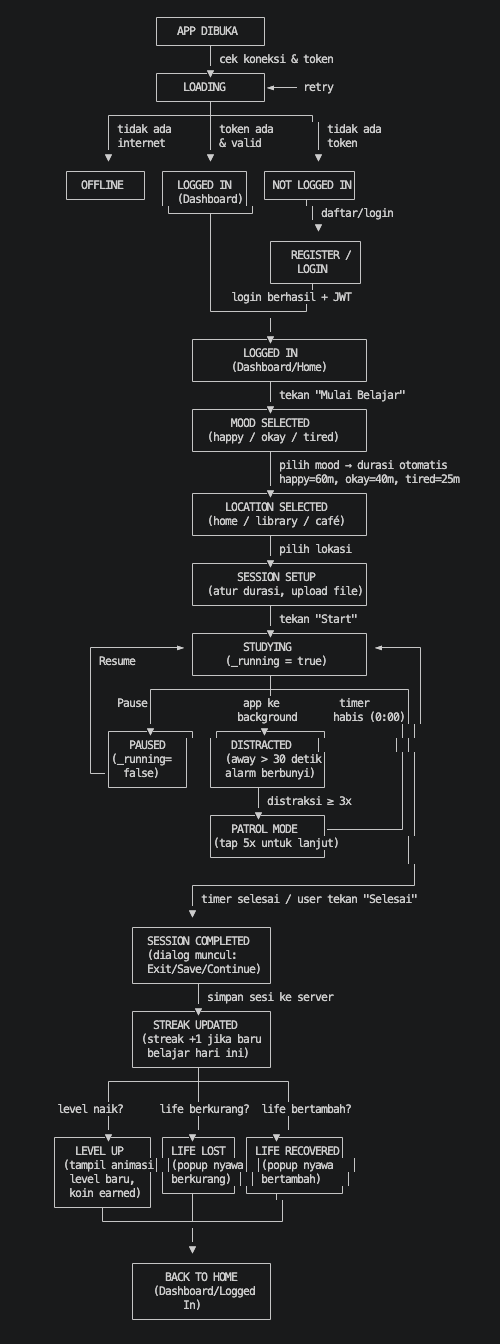
\includegraphics[
    width=\textwidth,
    height=0.8\textheight,
    keepaspectratio
]{state.png}

State Diagram menggambarkan perubahan status utama pengguna dan sesi belajar, seperti Not Logged In, Logged In, Mood Selected, Session Setup, Studying, Paused, Completed, Level Up, dan Streak Updated. Diagram ini penting untuk menjelaskan perubahan status aplikasi berdasarkan aktivitas pengguna. Penjelasan Kenapa Setiap Transisi Terjadi
  
  1. APP DIBUKA → LOADING
  Setiap kali app dibuka, sistem otomatis cek dua hal: apakah ada koneksi internet, dan apakah ada token login yang tersimpan. Ini
  mencegah user masuk ke dashboard kalau session-nya sudah kedaluwarsa.

  2. LOADING → NOT LOGGED IN / LOGGED IN / OFFLINE
  - Kalau tidak ada internet → masuk state OFFLINE, tidak bisa lanjut.
  - Kalau ada token valid → langsung ke dashboard tanpa perlu login ulang.
  - Kalau tidak ada token → diarahkan ke halaman login/register.

  3. LOGGED IN → MOOD SELECTED
  User memilih perasaannya sebelum belajar. Ini bukan sekadar kosmetik — mood langsung menentukan durasi belajar default: happy = 60
  menit, okay = 40 menit, tired = 25 menit. Kalau lagi capek, app tidak memaksa belajar lama.

  4. SESSION SETUP → STUDYING
  Setelah user konfirmasi durasi dan (opsional) upload file materi, timer dimulai dan state berubah menjadi running = true.

  5. STUDYING → PAUSE
  User menekan tombol Pause. Timer berhenti tapi tidak direset, jadi bisa dilanjutkan kapan saja.

  6. STUDYING → DISTRACTED
  Kalau user keluar dari app (pindah ke WhatsApp, Instagram, dll.) lebih dari 30 detik, alarm berbunyi. Ini fitur fokus — app
  mendeteksi lewat AppLifecycleState.paused/inactive.

  7. DISTRACTED → PATROL MODE
  Kalau user sudah terganggu 3 kali atau lebih, mode Patrol aktif. User harus tap layar 5 kali untuk membuktikan mereka sudah kembali
  Setiap kali app dibuka, sistem otomatis cek dua hal: apakah ada koneksi internet, dan apakah ada token login yang tersimpan. Ini
  mencegah user masuk ke dashboard kalau session-nya sudah kedaluwarsa.

  8. STUDYING → SESSION COMPLETED
  Terjadi dua cara:
  - Otomatis: timer countdown mencapai 0:00.
  - Manual: user tekan tombol "Selesai" lebih awal.

  9. SESSION COMPLETED → STREAK UPDATED
  Setelah sesi disimpan ke server, backend mengecek apakah user sudah belajar hari ini. Kalau belum, streak bertambah 1. Kalau sudah
  belajar sebelumnya hari ini, streak tidak berubah lagi.

  10. STREAK UPDATED → Coins
  Kalau Coins dari sesi ini membuat user naik level, muncul animasi Level Up dengan info level baru dan koin yang didapat.

  11. STREAK UPDATED → LIFE LOST / LIFE RECOVERED
  - Life berkurang: terjadi kalau user melewatkan hari belajar (dicek otomatis saat login oleh backend scheduler).
  - Life bertambah: terjadi kalau streak user kembali aktif setelah sempat turun.

  12. Semua → BACK TO HOME
  Setelah semua popup selesai, user kembali ke dashboard siap untuk sesi berikutnya.

\subsection{Component Diagram}

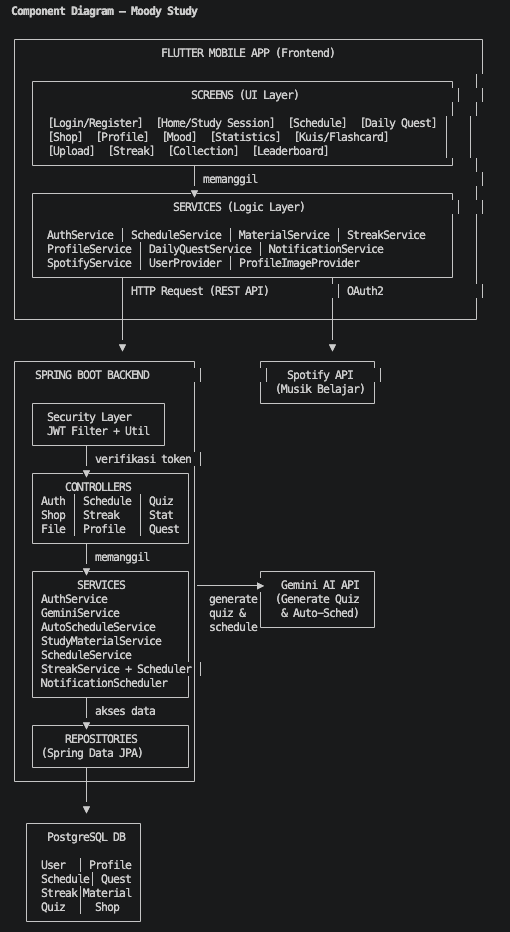
\includegraphics[
    width=\textwidth,
    height=0.8\textheight,
    keepaspectratio
]{component.png}

Component Diagram menggambarkan hubungan komponen utama sistem, yaitu Flutter Client, Authentication Module, Study Module, AI Service, Spotify Integration, Notification Service, Spring Boot REST API, dan PostgreSQL Database. Diagram ini digunakan untuk menunjukkan pembagian tanggung jawab antar komponen aplikasi.  Penjelasan Tiap Komponen

  1. Flutter Mobile App (Frontend)

  Ini adalah aplikasi yang dijalankan di HP pengguna. Terbagi menjadi dua lapisan:

  - Screens — tampilan yang dilihat pengguna (halaman login, belajar, jadwal, kuis, toko, dll.)
  - Services — logika di balik layar yang mengirim/menerima data ke server. Contoh: AuthService untuk login, ScheduleService untuk jadwal belajar.

  2. Spring Boot Backend (Server)

  Ini adalah otak dari aplikasi yang berjalan di server (202.46.28.170:8081). Terdiri dari tiga lapisan:

  - Security Layer (JWT) itu penjaga pintu. Setiap request dari app harus membawa token JWT yang valid, kalau tidak ditolak.
  - Controllers — penerima request. Misalnya /api/schedule ditangani ScheduleController.
  - Services — pemroses logika bisnis. Contoh: AutoScheduleService membuat jadwal otomatis, StreakMissedDayScheduler memotong streak jika user tidak belajar sehari.

  3. Repository + PostgreSQL

  Tempat menyimpan semua data pengguna secara permanen — akun, jadwal, streak, koin, materi, kuis, dll. Repository adalah jembatan antara kode Java dan database.

  4. Gemini AI API (Eksternal)

  Dipakai untuk dua fitur cerdas:
  - Generate kuis otomatis dari file materi yang di-upload user
  - Auto-schedule — membuat jadwal belajar secara otomatis berbasis AI

  5. Spotify API (Eksternal)

  Dipakai di fitur musik belajar — user bisa memutar playlist Spotify langsung dari dalam app.

  ---
  Alur singkat saat user login:

 HP → AuthService (Flutter) → POST /api/auth/login → JwtFilter → AuthController → AuthService (Spring) → UserRepository → PostgreSQL → balik JWT token → disimpan di HP untuk request selanjutnya.

\section{OOAD --- Design Patterns}

Beberapa design pattern yang dapat digunakan dalam pengembangan MOODY STUDY adalah sebagai berikut:

A) Pattern Singleton Category Creational. Singleton adalah membatasi jumlah objek yang dibuat agar hanya ada satu. JIka ada bagian lain dari program yang meminta objek ini, mereka semua akan mendapatkan objek yang sama. Dalam artian Memastikan sebuah class hanya memiliki satu instance, dan menyediakan titik akses global ke instance tersebut.

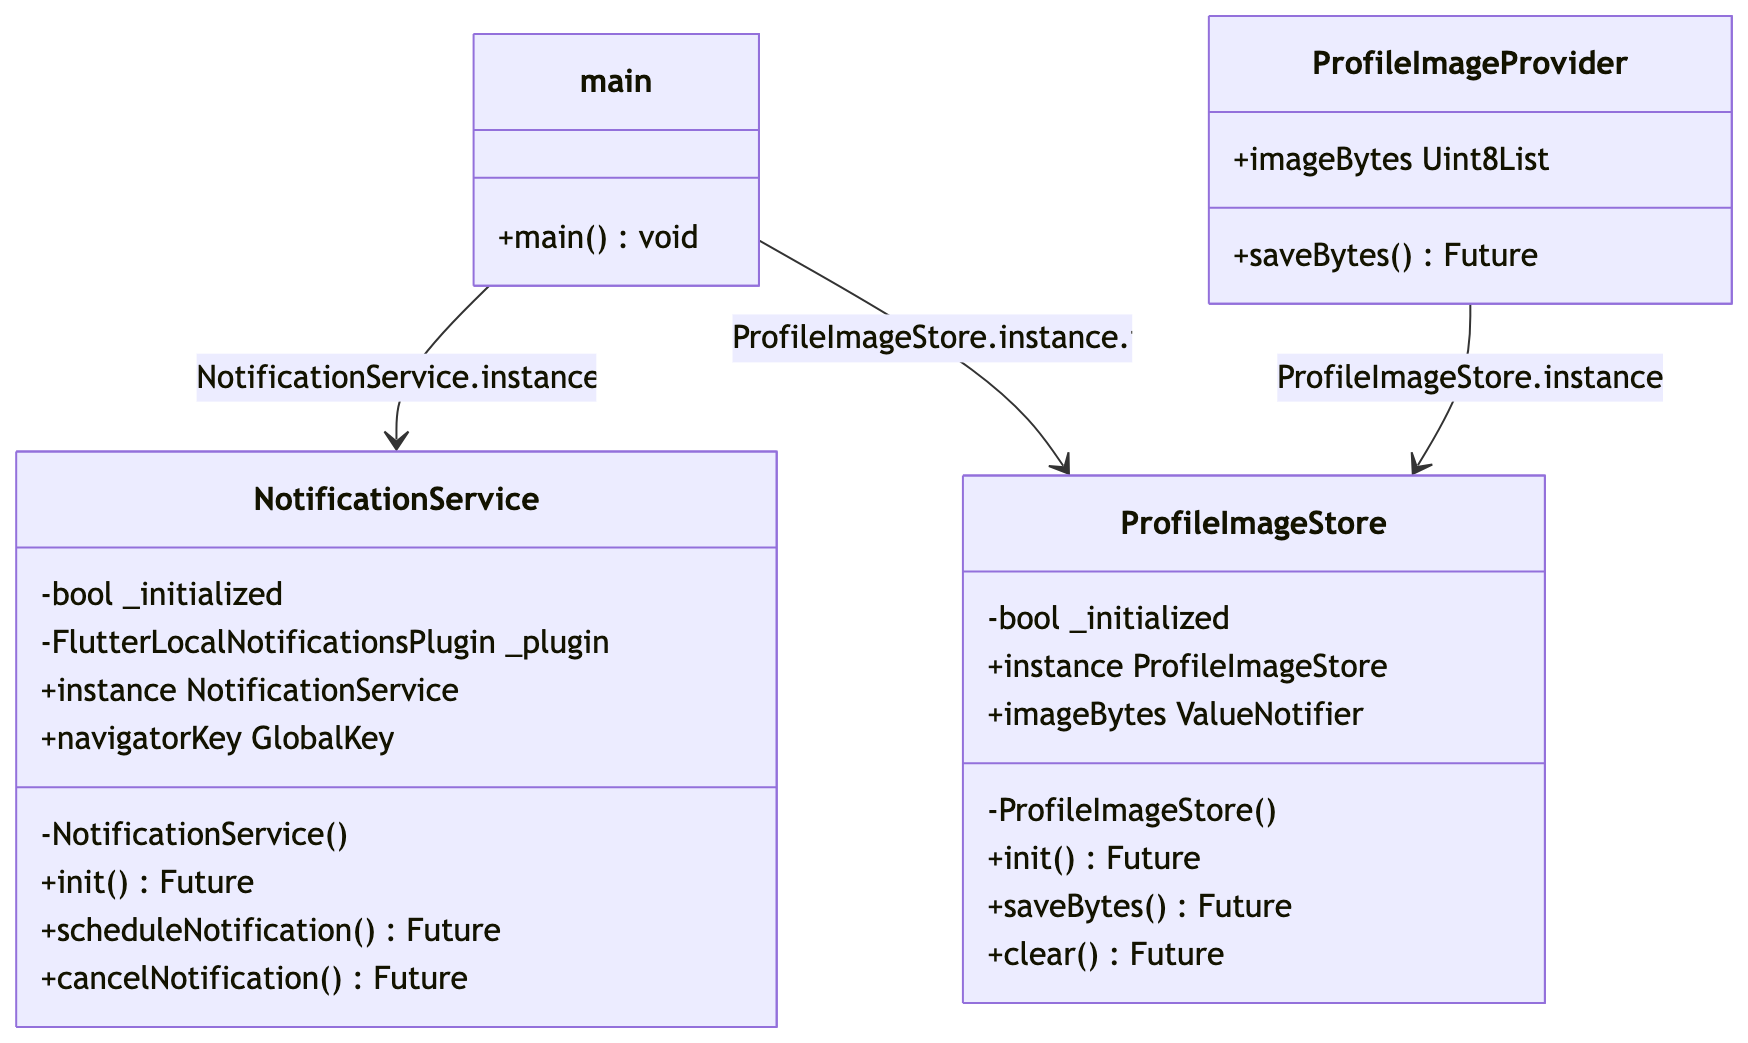
\includegraphics[
    width=\textwidth,
    height=0.8\textheight,
    keepaspectratio
]{singleton.png}

\begin{itemize}

\item \textbf{Primary Files}
\begin{itemize}
\item \texttt{moody\_study/lib/services/notification\_service.dart}
\item \texttt{moody\_study/lib/services/profile\_image\_store.dart}
\end{itemize}

\item \textbf{Related Files}
\begin{itemize}
\item \texttt{moody\_study/lib/main.dart}
\item \texttt{moody\_study/lib/services/profile\_image\_provider.dart}
\end{itemize}

\item \textbf{Classes Involved}
\begin{itemize}
\item \texttt{NotificationService} --- Singleton yang mengelola notifikasi aplikasi dan memastikan hanya terdapat satu instance yang aktif selama aplikasi berjalan.
\item \texttt{ProfileImageStore} --- Singleton yang bertanggung jawab mengelola penyimpanan dan pengambilan foto profil sehingga data tetap konsisten di seluruh aplikasi.
\end{itemize}
\end{itemize}

Cara Kerja Singleton pada Program Moody Study :
\begin{itemize}
    \item \textbf{Pembatasan Instansi (Restricting Quantity):} Kelas \texttt{NotificationService} dan \texttt{ProfileImageStore} memiliki atribut \textit{instance} statis yang menunjukkan bahwa hanya ada satu objek tunggal yang dikelola oleh kelas itu sendiri.

    \item \textbf{Constructor Privat:} Kedua kelas tersebut menggunakan constructor privat (ditandai dengan \texttt{-NotificationService()} dan \texttt{-ProfileImageStore()}). Hal ini memastikan kode dari luar (seperti kelas \texttt{main}) tidak dapat membuat objek baru menggunakan kata kunci \texttt{new} secara bebas.

    \item \textbf{Titik Akses Global (Global Access Point):} Kelas \texttt{main} dan \texttt{ProfileImageProvider} mengakses kedua layanan tersebut melalui \textit{instance} (misalnya \texttt{NotificationService.instance.init()}). Mekanisme ini menjadi satu pintu akses yang merupakan ciri khas pola Singleton.

    \item \textbf{Tujuan Penggunaan:} Implementasi ini sesuai dengan rekomendasi penggunaan Singleton untuk sumber daya penting seperti pengaturan sistem (\textit{registry settings}) atau penyimpanan memori (\textit{cache}), di mana keberadaan banyak instansi dapat menyebabkan inkonsistensi data dan perilaku sistem.
\end{itemize}

Alasan Memilih Pattern Singleton :
\begin{itemize}

\item \textbf{Masalah yang Diselesaikan:} \texttt{NotificationService} mengelola plugin notifikasi sistem (\texttt{flutter\_local\_notifications}) yang hanya boleh diinisialisasi satu kali dan memerlukan \texttt{GlobalKey<NavigatorState>} yang dibagikan ke seluruh aplikasi. \texttt{ProfileImageStore} menyimpan foto profil di memori dan disk. Jika terdapat lebih dari satu instance, widget yang berbeda dapat membaca data yang berbeda sehingga menyebabkan inkonsistensi pada antarmuka pengguna.

\item \textbf{Mengapa Pattern Ini Cocok:} Kedua kelas membutuhkan \textit{single point of truth}, yaitu satu instansi yang digunakan oleh seluruh aplikasi. Singleton menjamin tidak ada instansi ganda yang dapat menyebabkan \textit{race condition} maupun inkonsistensi state.

\item \textbf{Keuntungan yang Diperoleh:} Tidak terjadi inisialisasi ganda pada plugin notifikasi, data foto profil selalu sinkron di seluruh widget, serta layanan dapat diakses dari berbagai bagian aplikasi tanpa memerlukan \textit{dependency injection} secara manual.

\item \textbf{Mengapa Lebih Baik dari Pendekatan Sederhana:} Jika dibuat sebagai variabel global biasa, misalnya \texttt{var notifService = NotificationService();}, tidak ada enkapsulasi yang mencegah pembuatan instansi baru secara tidak sengaja. Jika objek dibuat setiap kali dibutuhkan menggunakan \texttt{NotificationService()}, plugin notifikasi dapat terinisialisasi berulang kali dan berpotensi menimbulkan error.

\item \textbf{Mengapa Bukan Pattern GoF Lain:} Implementasi ini bukan \textit{Factory} karena tidak ada variasi produk yang dibuat, bukan \textit{Builder} karena objek tidak dibangun melalui konfigurasi bertahap, dan bukan \textit{Prototype} karena tidak terdapat mekanisme cloning objek.

\end{itemize}

B) Pattern Adapter Category Structural. Adapter adalah mengubah antar muka (interface) suatu objek yang tidsak cocok menjadi antarmuka yang diharapkan oleh sistem. Dalam artian Mengkonversi interface sebuah class menjadi interface lain yang diharapkan oleh client. Adapter membuat class-class yang sebelumnya tidak kompatibel bisa bekerja bersama.

\includegraphics[
    width=\textwidth,
    height=0.8\textheight,
    keepaspectratio
]{Adapter.png}

\begin{itemize}
\item \textbf{Implementasi dalam Proyek}
\begin{itemize}
\item \textbf{Primary Files}
\begin{itemize}
    \item \texttt{moody\_study/lib/services/platform\_storage/storage\_io.dart}
    \item \texttt{moody\_study/lib/services/platform\_storage/storage\_web.dart}
\end{itemize}

\item \textbf{Related Files}
\begin{itemize}
    \item \texttt{moody\_study/lib/services/profile\_image\_store.dart} (\textit{Client})
\end{itemize}
\item \textbf{Classes Involved}
\begin{itemize}
    \item \texttt{StorageIOAdapter} --- Adapter untuk platform mobile dan desktop.
    \item \texttt{StorageWebAdapter} --- Adapter untuk platform web.
    \item \texttt{ProfileImageStore} --- Client yang menggunakan antarmuka target untuk mengakses penyimpanan lintas platform.
\end{itemize}
\end{itemize}
\end{itemize}


Cara Kerja Adapter pada Program Moody Study :
\begin{itemize}

\item \textbf{ProfileImageStore sebagai Klien:} Kelas \texttt{ProfileImageStore} menggunakan (\texttt{..> uses}) \texttt{TargetInterface}. Klien tidak perlu mengetahui bagaimana data disimpan secara teknis di bawahnya. Kelas ini hanya berinteraksi melalui operasi dasar seperti \texttt{save()}, \texttt{load()}, dan \texttt{clear()}, sehingga pemisahan tanggung jawab tetap terjaga.

\item \textbf{TargetInterface sebagai Antarmuka Ekspektasi:} \texttt{TargetInterface} mendefinisikan antarmuka yang diharapkan oleh sistem, seperti \texttt{platformSave()}, \texttt{platformLoad()}, dan \texttt{platformClear()}. Dengan adanya antarmuka ini, klien dapat bekerja tanpa bergantung pada implementasi penyimpanan tertentu.

\item \textbf{StorageIOAdapter dan StorageWebAdapter sebagai Adapter:} Kedua kelas tersebut mengimplementasikan (\texttt{<|.. implements}) \texttt{TargetInterface}. Sesuai dengan pola Adapter, kelas ini bertugas menerjemahkan permintaan dari antarmuka yang diharapkan sistem ke antarmuka yang dimiliki oleh platform penyimpanan yang sebenarnya.

\item \textbf{DartIOFile dan WebLocalStorage sebagai Adaptee:} Keduanya merupakan sistem penyimpanan bawaan yang memiliki antarmuka berbeda dan tidak kompatibel secara langsung. Sebagai contoh, \texttt{DartIOFile} menggunakan metode seperti \texttt{writeAsBytes()}, sedangkan \texttt{WebLocalStorage} menggunakan mekanisme \texttt{localStorage[]}.

\item \textbf{Relasi Adapts:} Adapter memiliki relasi menuju Adaptee melalui komposisi atau pembungkusan objek. Dengan cara ini, Adapter dapat mengubah antarmuka asli Adaptee sehingga sesuai dengan antarmuka yang diharapkan oleh klien tanpa perlu mengubah kode pada Adaptee maupun klien.

\end{itemize}

Alasan Memilih Pattern Adapter :
\begin{itemize}

\item \textbf{Masalah yang Diselesaikan:} Penyimpanan foto profil memerlukan API yang berbeda pada setiap platform. Platform mobile dan desktop menggunakan \texttt{dart:io} melalui kelas \texttt{File}, sedangkan platform web menggunakan \texttt{dart:html} melalui \texttt{localStorage}. Kedua API tersebut tidak kompatibel satu sama lain karena \texttt{dart:io} tidak tersedia pada browser dan \texttt{dart:html} tidak tersedia pada mobile. Namun, \texttt{ProfileImageStore} tetap membutuhkan operasi penyimpanan yang sama pada semua platform.

\item \textbf{Mengapa Pattern Ini Cocok:} Adapter merupakan solusi yang tepat untuk menyatukan dua antarmuka yang tidak kompatibel. Kelas \texttt{storage\_io.dart} dan \texttt{storage\_web.dart} bertindak sebagai adapter yang menerjemahkan API spesifik platform ke dalam antarmuka target yang seragam, yaitu \texttt{platformSave()}, \texttt{platformLoad()}, dan \texttt{platformClear()}. Dengan demikian, \texttt{ProfileImageStore} dapat bekerja tanpa mengetahui platform yang sedang digunakan.

\item \textbf{Keuntungan yang Diperoleh:} Kelas \texttt{ProfileImageStore} tidak perlu dimodifikasi ketika platform baru ditambahkan. Pengembang hanya perlu membuat adapter baru yang mengimplementasikan antarmuka yang sama. Selain itu, logika bisnis tetap bersih karena tidak dipenuhi oleh percabangan platform seperti \texttt{if (kIsWeb)}.

\item \textbf{Mengapa Lebih Baik dari Pendekatan Sederhana:} Tanpa Adapter, \texttt{ProfileImageStore} harus menggunakan kondisional platform pada setiap operasi penyimpanan dan pemuatan data, misalnya \texttt{if (kIsWeb) { localStorage...} else { File...}}. Pendekatan tersebut menyebabkan kelas menjadi \textit{tightly coupled} terhadap detail implementasi platform dan lebih sulit untuk diuji maupun dipelihara.

\item \textbf{Mengapa Bukan Pattern GoF Lain:} Implementasi ini bukan \textit{Strategy} karena pemilihan implementasi dilakukan berdasarkan platform saat proses kompilasi, bukan berdasarkan keputusan pengguna saat runtime. Implementasi ini juga bukan \textit{Decorator} karena tidak menambahkan perilaku baru pada objek, melainkan hanya mengubah antarmuka agar kompatibel. Selain itu, implementasi ini bukan \textit{Facade} karena tujuan utamanya adalah menyesuaikan antarmuka yang berbeda, bukan menyederhanakan subsystem yang kompleks.

\end{itemize}

C) Pattern Observer Category Behavioral. Observer adalah hubungan satu ke banyak itu maksudnya adalah satu Subject bisa memiliki banyak Observer sekaligus atau pemberitahuan perubahan status (state) secara otomatis. Dalam artian Mendefinisikan dependensi one-to-many antar objek, sehingga ketika satu objek berubah state, semua dependensinya dinotifikasi dan diupdate secara otomatis.

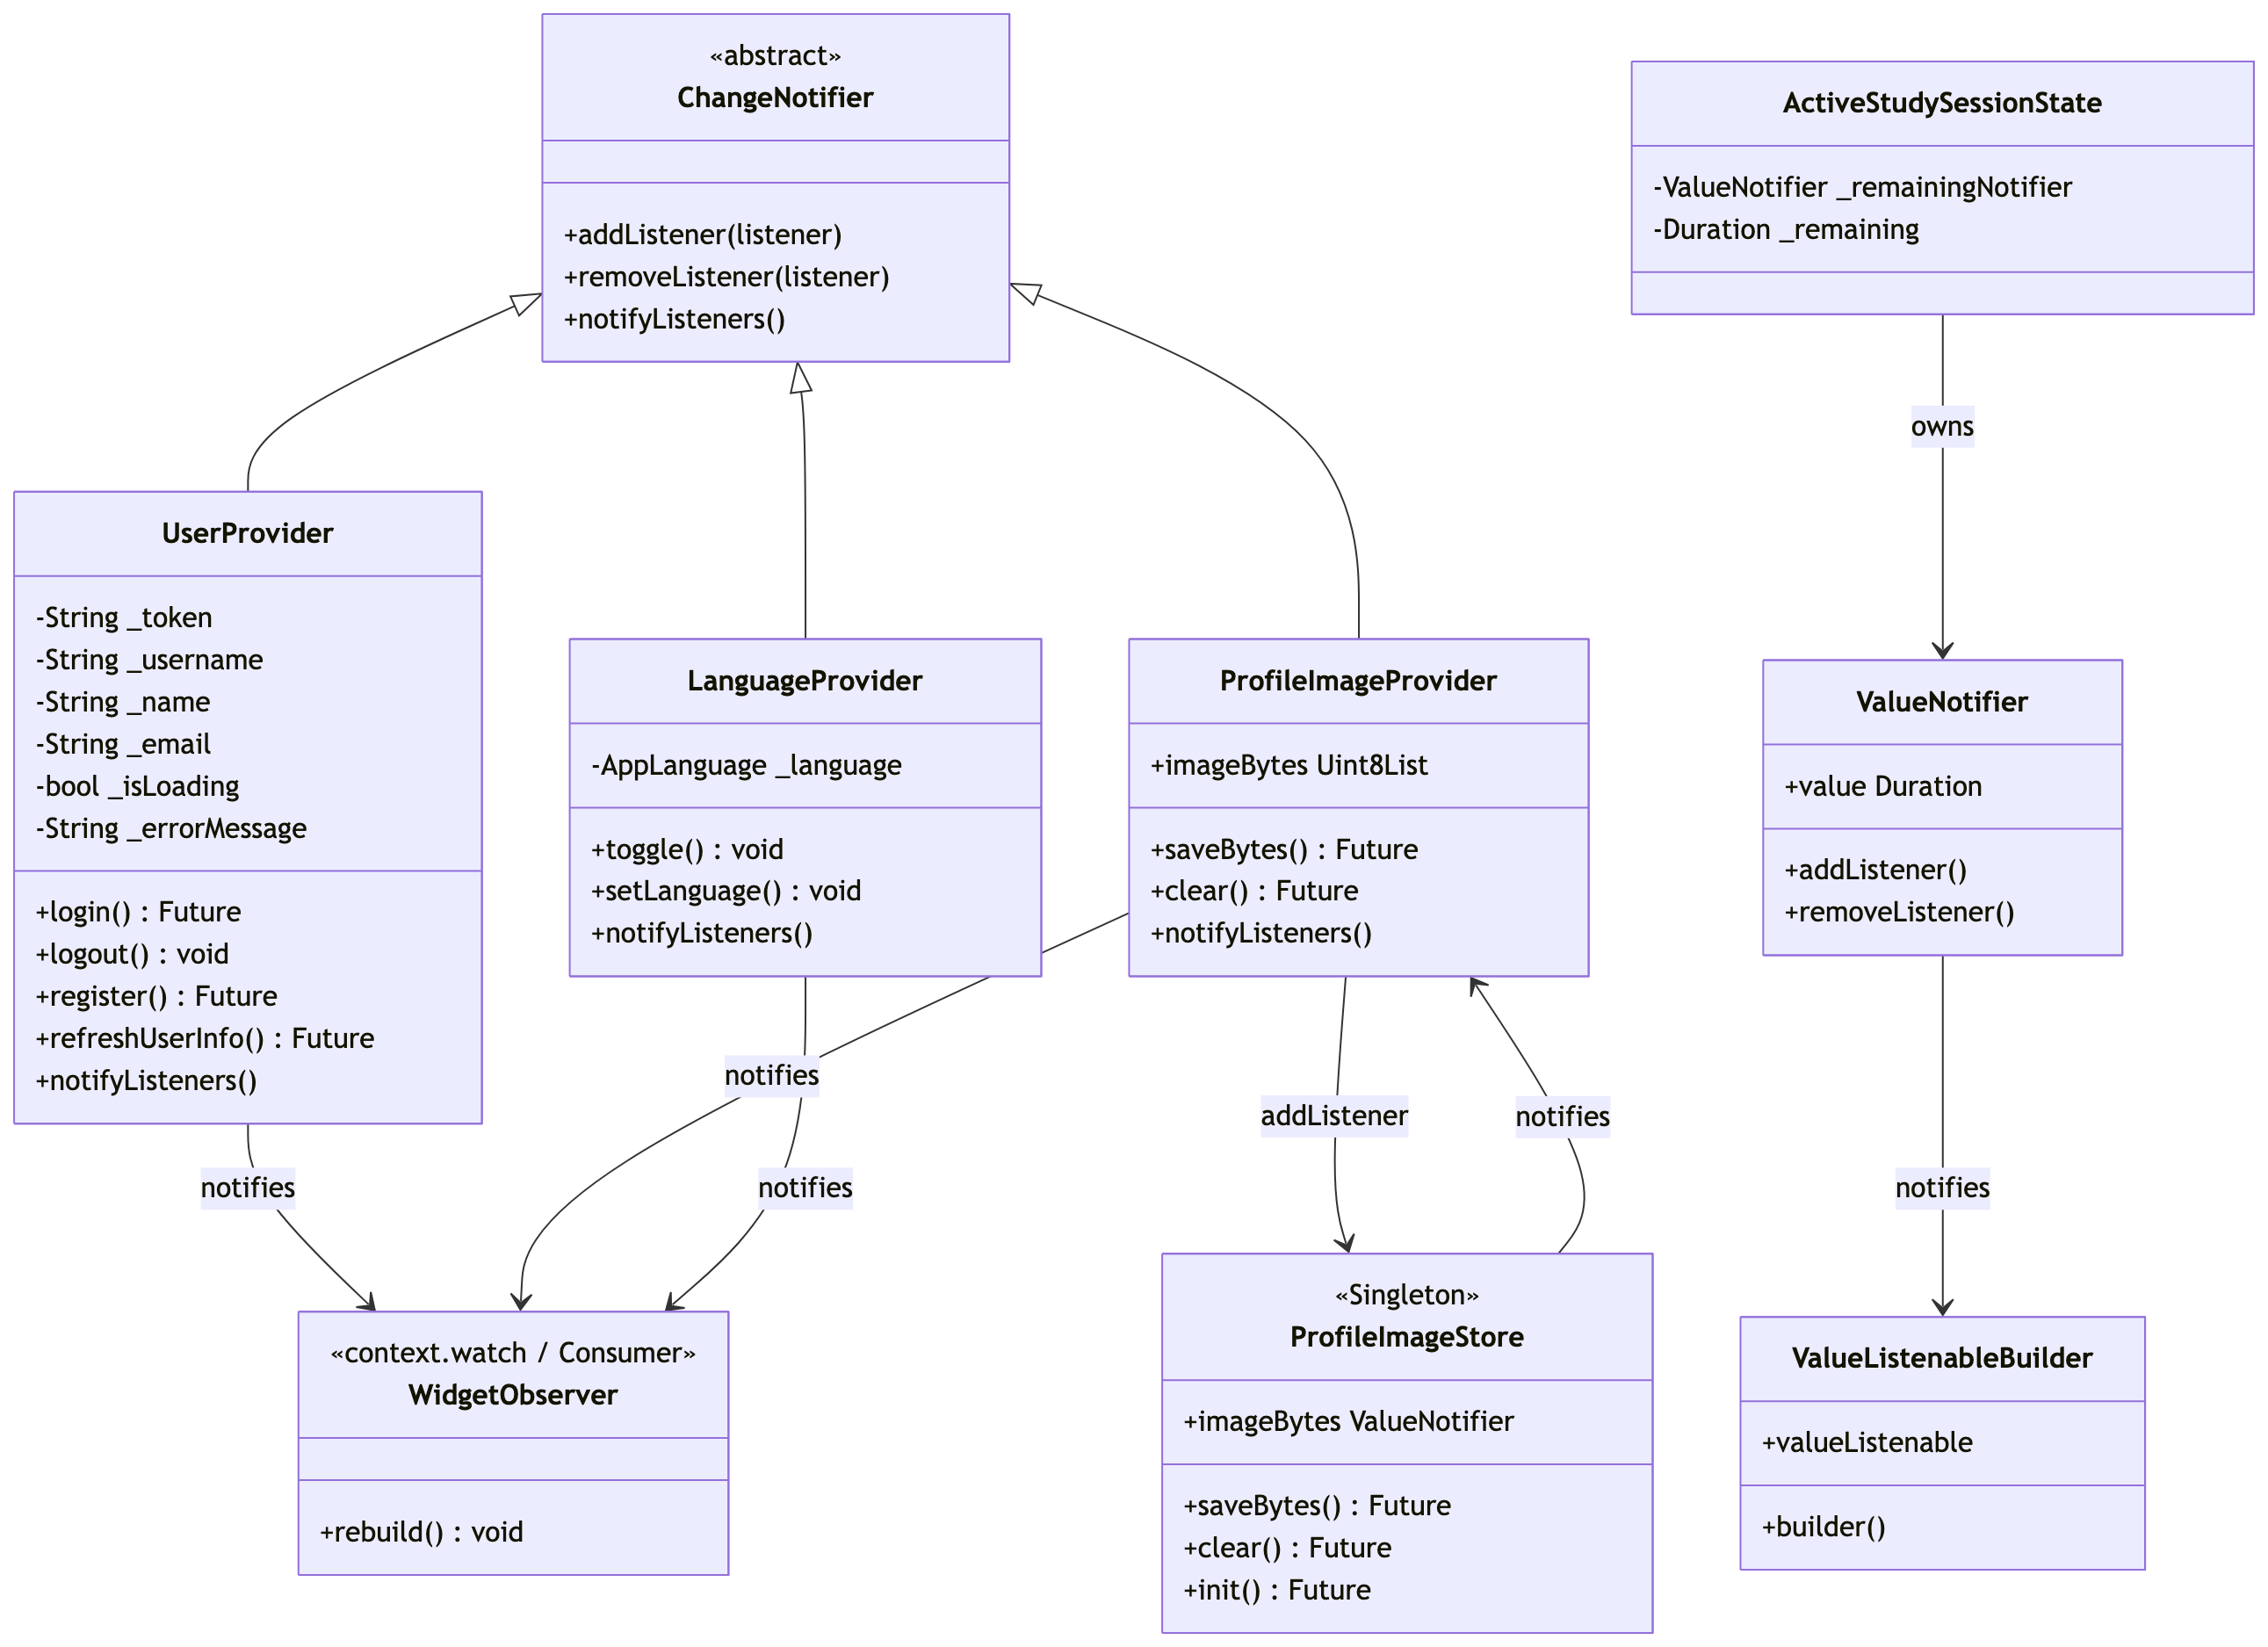
\includegraphics[
    width=\textwidth,
    height=0.8\textheight,
    keepaspectratio
]{Observer.png}

\begin{itemize}

\item \textbf{Primary Files}
\begin{itemize}
\item \texttt{moody\_study/lib/services/user\_provider.dart}
\item \texttt{moody\_study/lib/services/profile\_image\_provider.dart}
\item \texttt{moody\_study/lib/utils/app\_localizations.dart}
\end{itemize}
\item \textbf{Related Files}
\begin{itemize}
\item \texttt{moody\_study/lib/main.dart} --- Pendaftaran \textit{Subject} ke dalam \textit{Provider Tree}.
\item \texttt{moody\_study/lib/screens/active\_study\_session.dart} --- Implementasi \texttt{ValueNotifier} dan \texttt{ValueListenableBuilder} untuk pembaruan timer secara real\-time.
\item \texttt{moody\_study/lib/services/profile\_image\_store.dart} --- Menggunakan \texttt{ValueNotifier} sebagai \textit{Subject}.
\end{itemize}

\item \textbf{Classes Involved}
\begin{itemize}
\item \texttt{ChangeNotifier} --- \textit{Subject} (Observable) berupa antarmuka abstrak yang menyediakan mekanisme notifikasi kepada observer.
    \item \texttt{UserProvider} --- \textit{ConcreteSubject} yang mengelola perubahan data pengguna seperti login, logout, dan informasi profil.
    
    \item \texttt{ProfileImageProvider} --- \textit{ConcreteSubject} yang mengelola perubahan foto profil dan memberi notifikasi kepada widget yang bergantung padanya.
    
    \item \texttt{LanguageProvider} --- \textit{ConcreteSubject} yang mengelola perubahan bahasa aplikasi.
    
    \item \texttt{Consumer<T>} dan \texttt{context.watch<T>()} --- \textit{ConcreteObserver} yang berlangganan perubahan state dan melakukan rebuild secara otomatis ketika Subject berubah.
    
    \item \texttt{ValueNotifier<Duration>} --- \textit{Subject} khusus yang digunakan untuk mengelola perubahan nilai timer selama sesi belajar berlangsung.
    
    \item \texttt{ValueListenableBuilder<Duration>} --- \textit{Observer} yang mendengarkan perubahan pada \texttt{ValueNotifier<Duration>} dan memperbarui tampilan timer secara efisien.
\end{itemize}
\end{itemize}

Cara Kerja Observer pada Program Moody Study :
\begin{itemize}

\item \textbf{Satu Subjek ke Banyak Pengamat (One-to-Many):} Diagram menunjukkan bahwa \texttt{UserProvider}, \texttt{ProfileImageProvider}, dan \texttt{LanguageProvider} bertindak sebagai \textit{Subject} yang mengirimkan notifikasi kepada banyak \textit{Observer}. Mekanisme ini sesuai dengan konsep \textit{Observer Pattern}, di mana satu perubahan status pada subjek dapat disiarkan kepada banyak pengamat secara paralel.

\item \textbf{Mekanisme Interface (Loose Coupling):} Penggunaan \texttt{ChangeNotifier} sebagai kelas abstrak yang diwarisi oleh berbagai \textit{Provider} menunjukkan adanya keterkaitan yang longgar (\textit{loose coupling}). Subjek tidak perlu mengetahui implementasi detail dari pengamat, melainkan hanya menyediakan mekanisme notifikasi melalui antarmuka yang sama.

\item \textbf{Notifikasi Otomatis:} Ketika terjadi perubahan data atau status, seperti pada proses \texttt{login()}, \texttt{logout()}, atau \texttt{saveBytes()}, metode \texttt{notifyListeners()} akan dipanggil. Metode ini secara otomatis memberi tahu seluruh pengamat yang telah berlangganan sehingga antarmuka pengguna dapat diperbarui tanpa perlu pemanggilan manual.

\item \textbf{Struktur Observer pada Diagram:}
\begin{itemize}
\item \textbf{Subject:} \texttt{UserProvider}, \texttt{ProfileImageProvider}, \texttt{LanguageProvider}, dan \texttt{ValueNotifier}.
\item \textbf{Observer:} \texttt{WidgetObserver} (melalui \texttt{context.watch}) dan \texttt{ValueListenableBuilder}.
\item \textbf{Mekanisme Berlangganan:} Pengamat mendaftarkan diri menggunakan metode \texttt{addListener()}.
\item \textbf{Mekanisme Notifikasi:} Subjek menyiarkan perubahan kepada seluruh pengamat menggunakan metode \texttt{notifyListeners()}.
\end{itemize}
\end{itemize}

Alasan Memilih Pattern Observer :
\begin{itemize}

\item \textbf{Masalah yang Diselesaikan:} Banyak widget pada berbagai layar aplikasi perlu bereaksi terhadap perubahan data, seperti proses login, logout, pembaruan profil pengguna, perubahan foto profil, maupun pergantian bahasa. Tanpa mekanisme khusus, setiap widget harus terhubung secara langsung dengan sumber data, yang dapat meningkatkan kompleksitas dan ketergantungan antar komponen.

\item \textbf{Mengapa Observer Cocok:} Observer Pattern memungkinkan perubahan state pada satu objek \textit{Subject} untuk secara otomatis diteruskan kepada seluruh \textit{Observer} yang bergantung padanya. Dengan pendekatan ini, \textit{Subject} tidak perlu mengetahui siapa saja pengamatnya, sehingga hubungan antar komponen tetap longgar (\textit{loosely coupled}).

\item \textbf{Keuntungan yang Diperoleh:} Antarmuka pengguna selalu sinkron dengan data terbaru tanpa memerlukan pembaruan manual pada setiap layar. Pengembang tidak perlu memanggil \texttt{setState()} secara berulang pada berbagai widget. Selain itu, performa aplikasi dapat ditingkatkan melalui penggunaan \texttt{RepaintBoundary} dan \texttt{ValueListenableBuilder}, sehingga hanya komponen tertentu, seperti timer, yang akan dibangun ulang (\textit{rebuild}) ketika terjadi perubahan.

\item \textbf{Mengapa Lebih Baik dari Pendekatan Sederhana:} Tanpa Observer Pattern, setiap layar harus melakukan \textit{polling} data secara berkala atau menerima callback secara manual dari berbagai sumber data. Pendekatan tersebut dapat menghasilkan ketergantungan yang kompleks (\textit{spaghetti dependency}), meningkatkan biaya pemeliharaan kode, dan menyulitkan pengembangan fitur baru.

\item \textbf{Mengapa Bukan Pattern GoF Lain:} Implementasi ini bukan \textit{Mediator} karena \textit{Subject} dan \textit{Observer} tidak saling berkoordinasi melalui objek perantara yang mengatur komunikasi dua arah. Implementasi ini juga bukan \textit{Event Bus} karena tidak terdapat \textit{central event dispatcher} yang bertugas menerima dan mendistribusikan seluruh event aplikasi. Fokus utama implementasi ini adalah notifikasi otomatis dari \textit{Subject} kepada \textit{Observer} yang telah berlangganan.

\end{itemize}

D) Pattern CHAIN OF RESPONSIBILITY Category Behavioral. CHAIN OF RESPONSIBILITY adalah pola desain yang memberikan kesempatan kepada lebih dari satu objek untuk menangani suatu permintaan dengan cara meneruskannya sepanjang rantai urutan objek tersebut. Dalam artian Menghindari coupling antara pengirim request dan penerimanya dengan memberi lebih dari satu objek kesempatan untuk menangani request. Chain objek penerima dan pass request sepanjang chain sampai ada yang menanganinya.

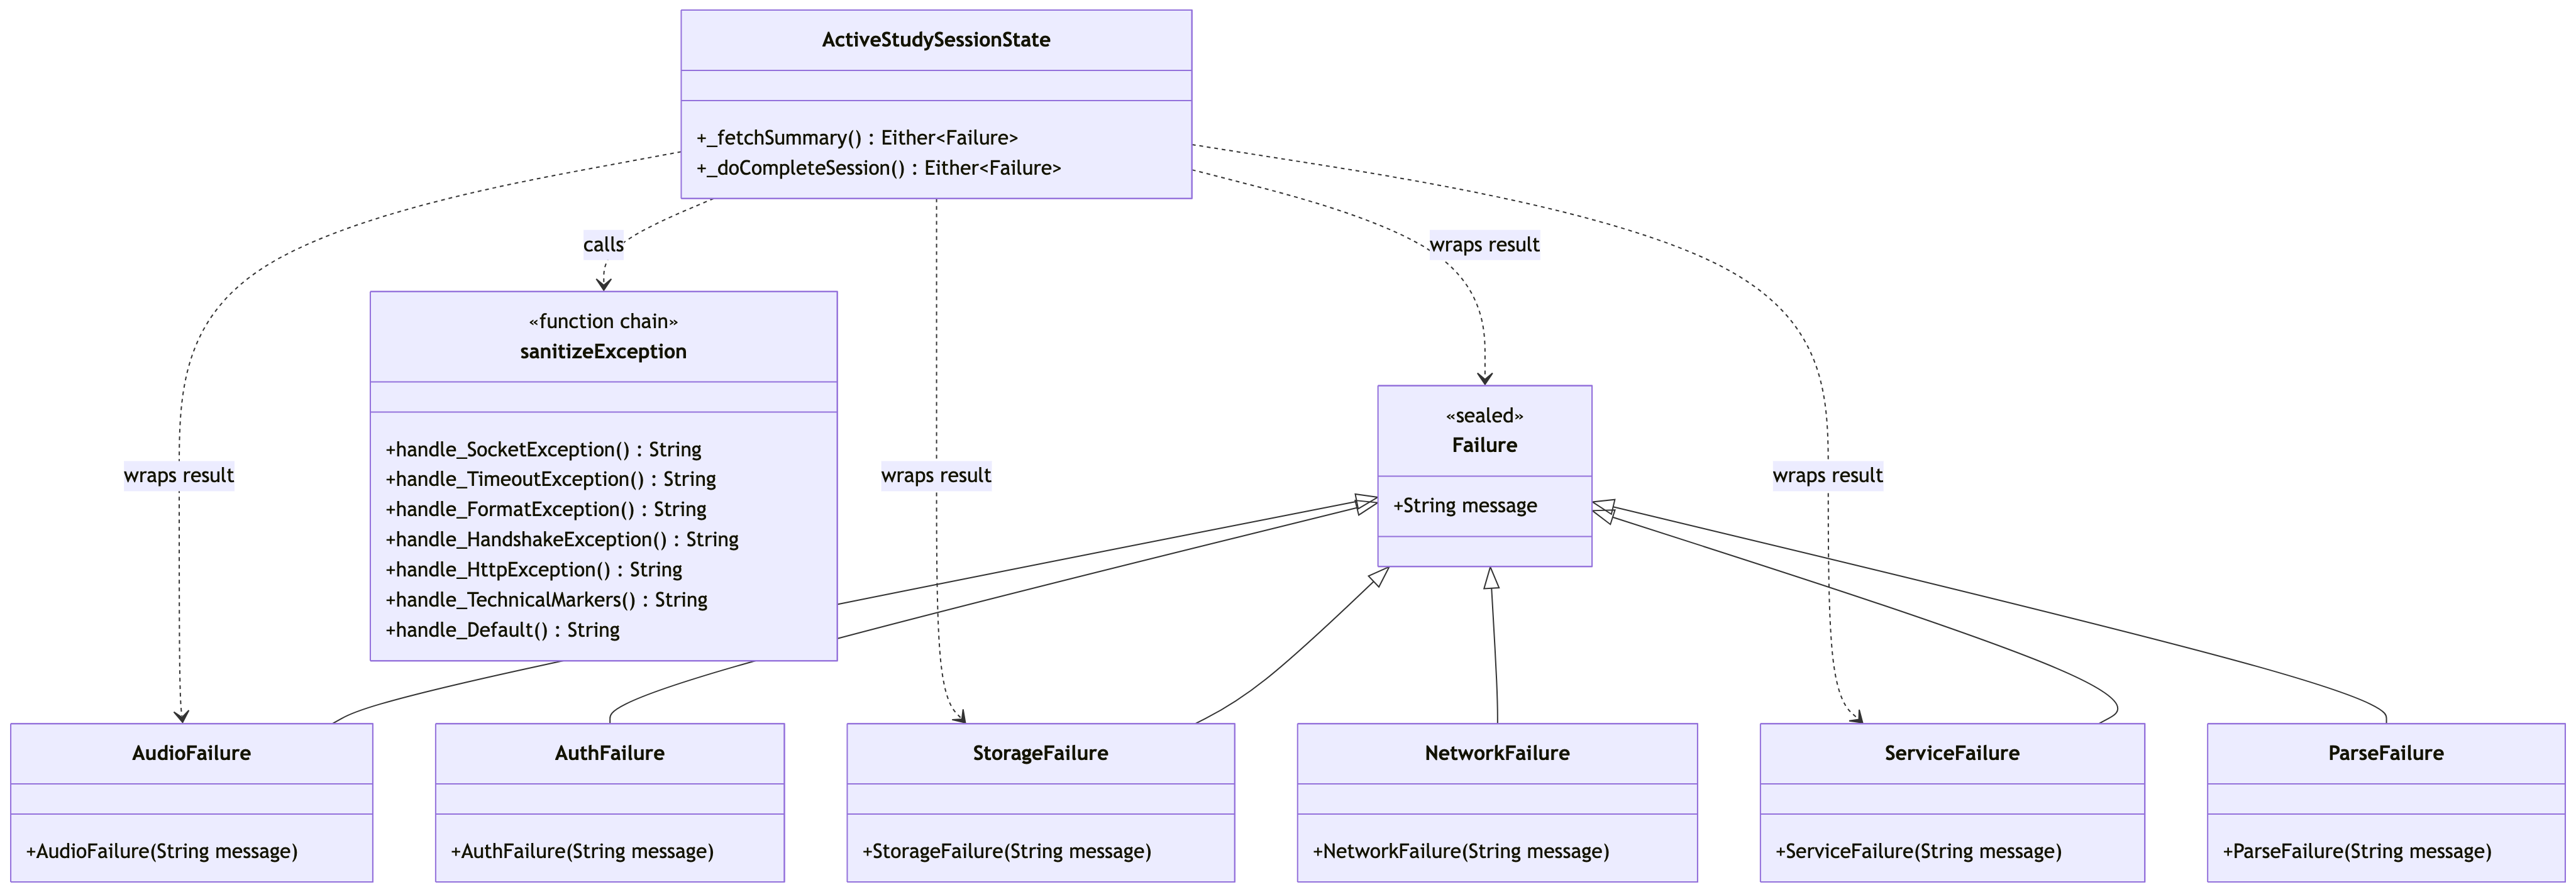
\includegraphics[
    width=\textwidth,
    height=0.8\textheight,
    keepaspectratio
]{chainpattern.png}

\begin{itemize}

\item \textbf{Primary Files}
\begin{itemize}
\item \texttt{moody\_study/lib/core/exception\_handler.dart}
\item \texttt{moody\_study/lib/core/failure.dart}
\end{itemize}

\item \textbf{Related Files}
\begin{itemize}
\item \texttt{moody\_study/lib/services/auth\_service.dart} --- Menggunakan rantai penanganan exception (\textit{chain}).

    \item \texttt{moody\_study/lib/screens/active\_study\_session.dart} --- Memanggil fungsi \texttt{sanitizeException()} untuk mengonversi exception menjadi \textit{Failure} yang ramah pengguna.
    
    \item \texttt{moody\_study/lib/screens/study\_session.dart} --- Memanfaatkan \texttt{sanitizeException()} untuk menangani exception secara terpusat.
\end{itemize}

\item \textbf{Classes Involved}
\begin{itemize}
\item \texttt{sanitizeException(Object e)} --- \textit{Chain Orchestrator} yang meneruskan exception melalui serangkaian handler hingga ditemukan penanganan yang sesuai.

    \item \texttt{Failure} (\textit{sealed class}) --- Tipe dasar (\textit{base handler result}) yang merepresentasikan hasil akhir dari proses penanganan exception.
    
    \item \texttt{AuthFailure} --- \textit{Concrete Handler Result} untuk kegagalan autentikasi.
    
    \item \texttt{NetworkFailure} --- \textit{Concrete Handler Result} untuk kesalahan jaringan atau koneksi.
    
    \item \texttt{AudioFailure} --- \textit{Concrete Handler Result} untuk kesalahan yang berkaitan dengan pemutaran atau pengelolaan audio.
    
    \item \texttt{StorageFailure} --- \textit{Concrete Handler Result} untuk kesalahan penyimpanan data atau akses berkas.
    
    \item \texttt{ServiceFailure} --- \textit{Concrete Handler Result} untuk kegagalan layanan eksternal maupun layanan internal aplikasi.
    
    \item \texttt{ParseFailure} --- \textit{Concrete Handler Result} untuk kesalahan parsing atau konversi data.
\end{itemize}

\end{itemize}

Cara Kerja CHAIN OF RESPONSIBILITY pada Program Moody Study :
\begin{itemize}

\item \textbf{Alur Sekuensial (The Relay):} Chain of Responsibility (CoR) bekerja seperti estafet, di mana suatu permintaan diteruskan dari satu penangan (\textit{handler}) ke penangan berikutnya hingga ditemukan yang mampu memprosesnya. Pada implementasi ini, fungsi \texttt{sanitizeException()} memeriksa berbagai jenis exception secara berurutan, seperti \texttt{SocketException}, \texttt{TimeoutException}, dan exception lainnya, hingga mencapai \texttt{handle\_Default()} apabila tidak ada handler yang sesuai.

\item \textbf{Pemisahan Pengirim dan Penerima:} Pola CoR memisahkan objek pengirim permintaan dari objek yang bertanggung jawab menanganinya. Dalam diagram, \texttt{ActiveStudySessionState} bertindak sebagai pengirim yang tidak perlu mengetahui detail logika penanganan exception. Kelas tersebut hanya memanggil \texttt{sanitizeException()} dan menerima hasil yang telah diproses.

\item \textbf{Banyak Objek Memiliki Kesempatan Menangani:} Salah satu karakteristik utama CoR adalah memberikan kesempatan kepada beberapa handler untuk menangani suatu permintaan. Pada implementasi ini, setiap jenis exception memiliki peluang untuk diperiksa oleh handler yang sesuai dalam rantai penanganan sebelum diteruskan ke handler berikutnya.

\item \textbf{Berhenti Saat Permintaan Ditangani:} Permintaan akan terus diteruskan sepanjang rantai hingga ditemukan handler yang mampu menanganinya. Setelah exception berhasil dipetakan ke pesan yang sesuai, proses penelusuran rantai akan dihentikan. Jika tidak ada handler spesifik yang cocok, maka penanganan akan dialihkan ke \texttt{handle\_Default()} sebagai penangan terakhir.

\end{itemize}

Alasan Memilih Pattern CHAIN OF RESPONSIBILITY :
\begin{itemize}

\item \textbf{Masalah yang Diselesaikan:} Aplikasi perlu menangani berbagai jenis exception yang berasal dari beragam sumber, seperti jaringan, sistem berkas (\textit{file system}), audio, dan layanan HTTP. Selain itu, pesan error yang ditampilkan kepada pengguna harus mudah dipahami serta tidak mengandung informasi teknis sensitif seperti alamat IP, nomor port, URL, atau detail internal sistem.

\item \textbf{Mengapa Chain of Responsibility Cocok:} Setiap jenis exception memerlukan penanganan yang berbeda. Chain of Responsibility memungkinkan exception diproses secara berurutan oleh serangkaian handler. Jika handler pertama tidak dapat menangani exception tersebut, permintaan akan diteruskan ke handler berikutnya hingga ditemukan handler yang sesuai.

\item \textbf{Keuntungan yang Diperoleh:} Komponen pemanggil, seperti \texttt{\_fetchSummary()}, \texttt{\_tryPauseMusicPlayer()}, dan metode lainnya, tidak perlu mengetahui jenis exception yang mungkin muncul. Seluruh logika penanganan terpusat dalam satu rantai handler. Ketika diperlukan penanganan exception baru, pengembang cukup menambahkan handler baru tanpa harus mengubah kode pada seluruh pemanggil.

\item \textbf{Mengapa Lebih Baik dari Pendekatan Sederhana:} Jika setiap metode menggunakan blok \texttt{try-catch} untuk seluruh jenis exception secara terpisah, akan terjadi duplikasi kode dalam jumlah besar dan proses pemeliharaan menjadi lebih sulit. Sebaliknya, jika hanya menggunakan satu handler umum tanpa rantai penanganan, aplikasi hanya dapat menampilkan pesan generik yang kurang informatif bagi pengguna.

\item \textbf{Mengapa Bukan Pattern GoF Lain:} Implementasi ini bukan \textit{Strategy} karena tidak memilih satu algoritma tertentu untuk dijalankan, melainkan mencoba beberapa handler secara berurutan hingga ditemukan yang sesuai. Implementasi ini juga bukan \textit{Command} karena tidak mengenkapsulasi operasi sebagai objek yang dapat dieksekusi atau di-\textit{undo}. Selain itu, implementasi ini bukan \textit{Visitor} karena tidak bertujuan memisahkan operasi dari struktur objek yang dikunjungi.
\end{itemize}

E) Pattern Facade Category Structural. Facade adalah  Menyediakan interface yang terpadu (unified) ke sekumpulan interface dalam sebuah subsystem. Facade mendefinisikan interface higher-level yang membuat subsystem lebih mudah digunakan. Dalam artian menyederhanakan interaksi dengan sistem yang kompleks.

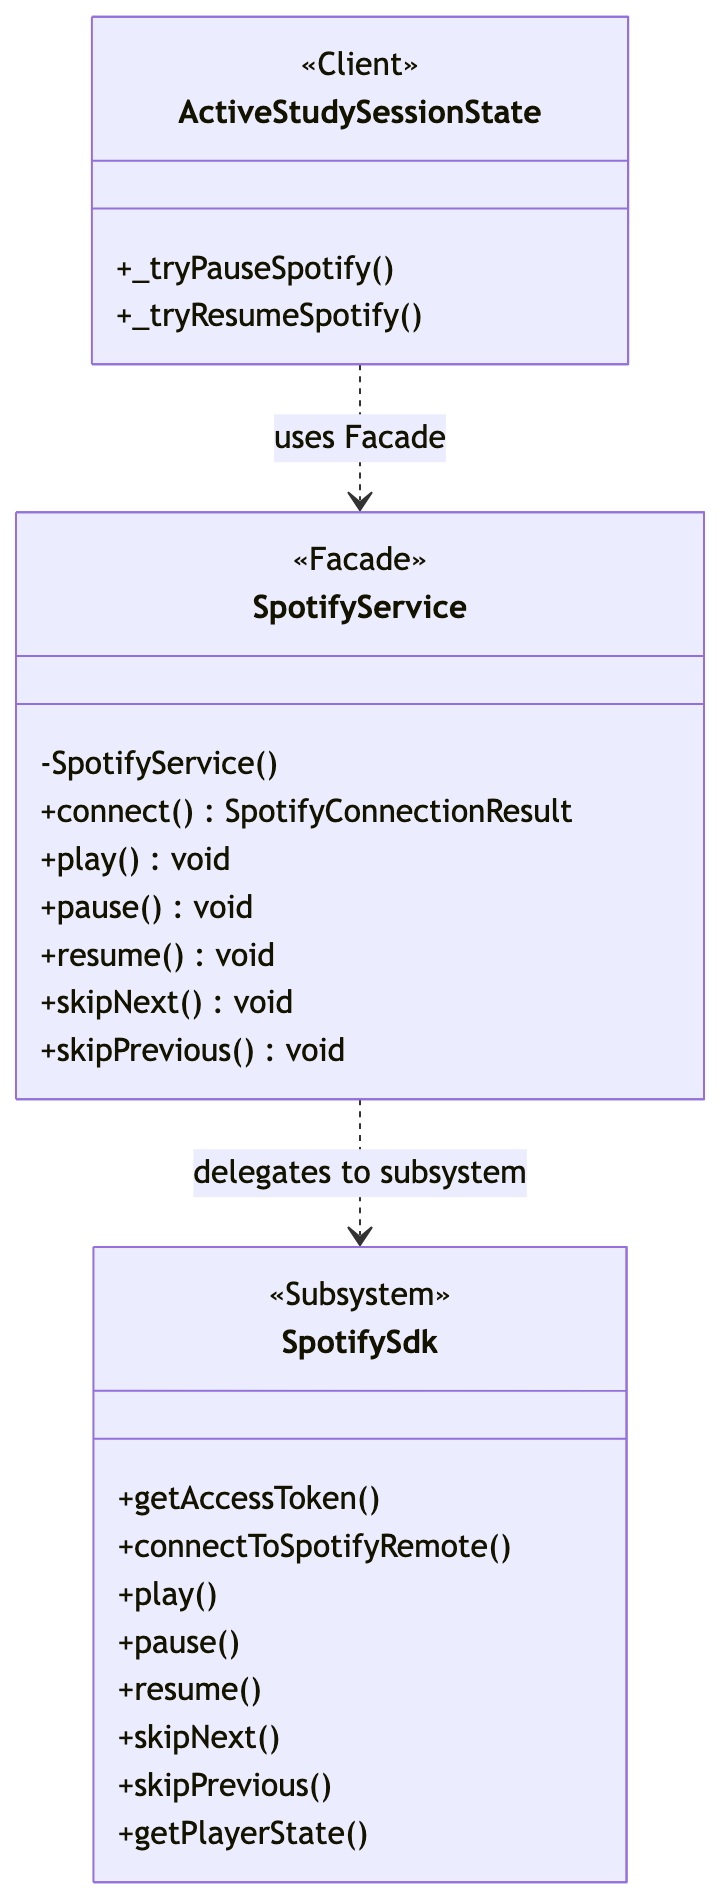
\includegraphics[
    width=\textwidth,
    height=0.8\textheight,
    keepaspectratio
]{facadee.png}
\begin{itemize}

\item \textbf{Primary File}
\begin{itemize}
\item \texttt{moody\_study/lib/services/spotify\_service.dart}
\end{itemize}

\item \textbf{Related Files}
\begin{itemize}
\item \texttt{moody\_study/lib/screens/active\_study\_session.dart} --- Bertindak sebagai \textit{client} yang menggunakan layanan Spotify selama sesi belajar berlangsung.

    \item \texttt{moody\_study/lib/screens/headphone\_screen.dart} --- Bertindak sebagai \textit{client} yang berinteraksi dengan layanan Spotify untuk pengelolaan musik dan perangkat audio.
\end{itemize}

\item \textbf{Classes Involved}
\begin{itemize}
\item \texttt{SpotifyService} --- \textit{Facade} yang menyediakan antarmuka sederhana untuk mengakses berbagai fitur Spotify tanpa mengekspos kompleksitas SDK yang mendasarinya.

    \item \texttt{SpotifySdk} (\texttt{package:spotify\_sdk}) --- \textit{Subsystem} yang berisi implementasi API Spotify, termasuk autentikasi, koneksi, dan kontrol pemutaran musik.
    
    \item \texttt{\_ActiveStudySessionState} --- \textit{Client} yang memanfaatkan \texttt{SpotifyService} untuk mengelola musik selama sesi belajar aktif.
\end{itemize}
\end{itemize}

Cara Kerja Facade pada Program Moody Study :
\begin{itemize}

\item \textbf{Penyederhanaan Antarmuka (Simplify):} \texttt{SpotifyService} berperan sebagai \textit{Facade} dengan menyediakan antarmuka yang sederhana dan mudah digunakan, seperti \texttt{connect()}, \texttt{play()}, \texttt{pause()}, dan operasi lainnya. Dengan demikian, klien tidak perlu berinteraksi langsung dengan berbagai fungsi kompleks yang terdapat pada subsistem Spotify.

\item \textbf{Pemisahan Subsistem yang Kompleks:} \texttt{SpotifySdk} pada diagram berfungsi sebagai \textit{subsystem} yang terdiri dari berbagai proses dan API yang kompleks. Facade digunakan untuk menyembunyikan kompleksitas tersebut sehingga komponen lain dalam aplikasi dapat berinteraksi melalui antarmuka yang lebih sederhana dan terstruktur.

\item \textbf{Delegasi Tugas:} \texttt{SpotifyService} tidak menjalankan seluruh logika secara mandiri, melainkan mendelegasikan pekerjaan kepada komponen-komponen yang terdapat di dalam \texttt{SpotifySdk}. Facade bertindak sebagai perantara yang menerima permintaan dari klien dan meneruskannya ke subsistem yang sesuai.

\item \textbf{Prinsip Pengetahuan Minimum (Principle of Least Knowledge):} \texttt{ActiveStudySessionState} sebagai klien hanya perlu berinteraksi dengan \texttt{SpotifyService}. Klien tidak perlu mengetahui detail implementasi, struktur internal, maupun alur komunikasi yang terdapat di dalam \texttt{SpotifySdk}. Pendekatan ini mengurangi ketergantungan antar komponen dan meningkatkan keterpeliharaan sistem.

\item \textbf{Tujuan Penggunaan Facade:} Pattern Facade digunakan karena subsistem yang mendasarinya memiliki proses yang cukup kompleks dan melibatkan banyak langkah. Dengan menyediakan satu titik akses yang sederhana, Facade membantu menyederhanakan penggunaan subsistem sekaligus mengurangi kompleksitas yang harus dipahami oleh klien.

\end{itemize}

Alasan Memilih Pattern Facade :
\begin{itemize}

\item \textbf{Masalah yang Diselesaikan:} Integrasi dengan \texttt{SpotifySdk} memerlukan serangkaian proses yang kompleks, seperti memperoleh token autentikasi, melakukan koneksi ke layanan Spotify, mengelola pemutaran musik, menangani error, mengatur timeout, serta memvalidasi token yang digunakan. Jika setiap layar (\textit{screen}) menangani proses ini secara langsung, akan terjadi duplikasi kode dan peningkatan kompleksitas pada berbagai bagian aplikasi.

\item \textbf{Mengapa Facade Cocok:} \texttt{SpotifyService} bertindak sebagai \textit{Facade} yang menyembunyikan seluruh kompleksitas interaksi dengan \texttt{SpotifySdk}. Kelas ini menyediakan antarmuka yang sederhana dan mudah digunakan, seperti \texttt{connect()}, \texttt{play()}, dan \texttt{pause()}, sehingga klien tidak perlu memahami detail implementasi subsistem di belakangnya.

\item \textbf{Keuntungan yang Diperoleh:} Seluruh logika integrasi dengan Spotify terpusat pada \texttt{SpotifyService}, sehingga kode menjadi lebih terstruktur dan mudah dipelihara. Apabila terjadi perubahan pada \texttt{SpotifySdk}, hanya implementasi di dalam \texttt{SpotifyService} yang perlu diperbarui, sementara seluruh klien yang menggunakannya tetap dapat bekerja tanpa modifikasi tambahan.

\item \textbf{Mengapa Lebih Baik dari Pendekatan Sederhana:} Tanpa Facade, setiap layar harus mengelola proses autentikasi, koneksi, pemutaran musik, dan penanganan error secara mandiri. Hal ini menyebabkan duplikasi kode, meningkatkan risiko inkonsistensi implementasi, serta menyulitkan proses pemeliharaan ketika terjadi perubahan pada SDK yang digunakan.

\item \textbf{Mengapa Bukan Pattern GoF Lain:} Implementasi ini bukan \textit{Adapter} karena tidak bertujuan mengubah antarmuka yang tidak kompatibel menjadi kompatibel. Implementasi ini juga bukan \textit{Mediator} karena tidak mengatur komunikasi antar objek yang saling berinteraksi. Fokus utama pattern ini adalah menyederhanakan akses terhadap subsistem yang kompleks melalui satu titik masuk yang mudah digunakan.
\end{itemize}

\section{OOAD --- Traceability Audit}

Traceability audit digunakan untuk memastikan setiap kebutuhan sistem memiliki hubungan yang jelas dengan rancangan dan implementasi kode. Tabel berikut merangkum pemetaan desain ke komponen implementasi.

\renewcommand{\arraystretch}{1.5}
\setlength{\tabcolsep}{8pt}

\begin{longtable}{|m{0.20\textwidth}|p{0.72\textwidth}|}
\caption{Bukti Implementasi Design Pattern pada Moody Study}
\label{tab:design_pattern_evidence}\\
\hline
\textbf{Pattern} & \textbf{Bukti Code} \\
\hline
\endfirsthead

\hline
\textbf{Pattern} & \textbf{Bukti Code} \\
\hline
\endhead

Singleton &
\begin{minipage}[t]{0.70\textwidth}
    \vspace{1ex}
    \centering
    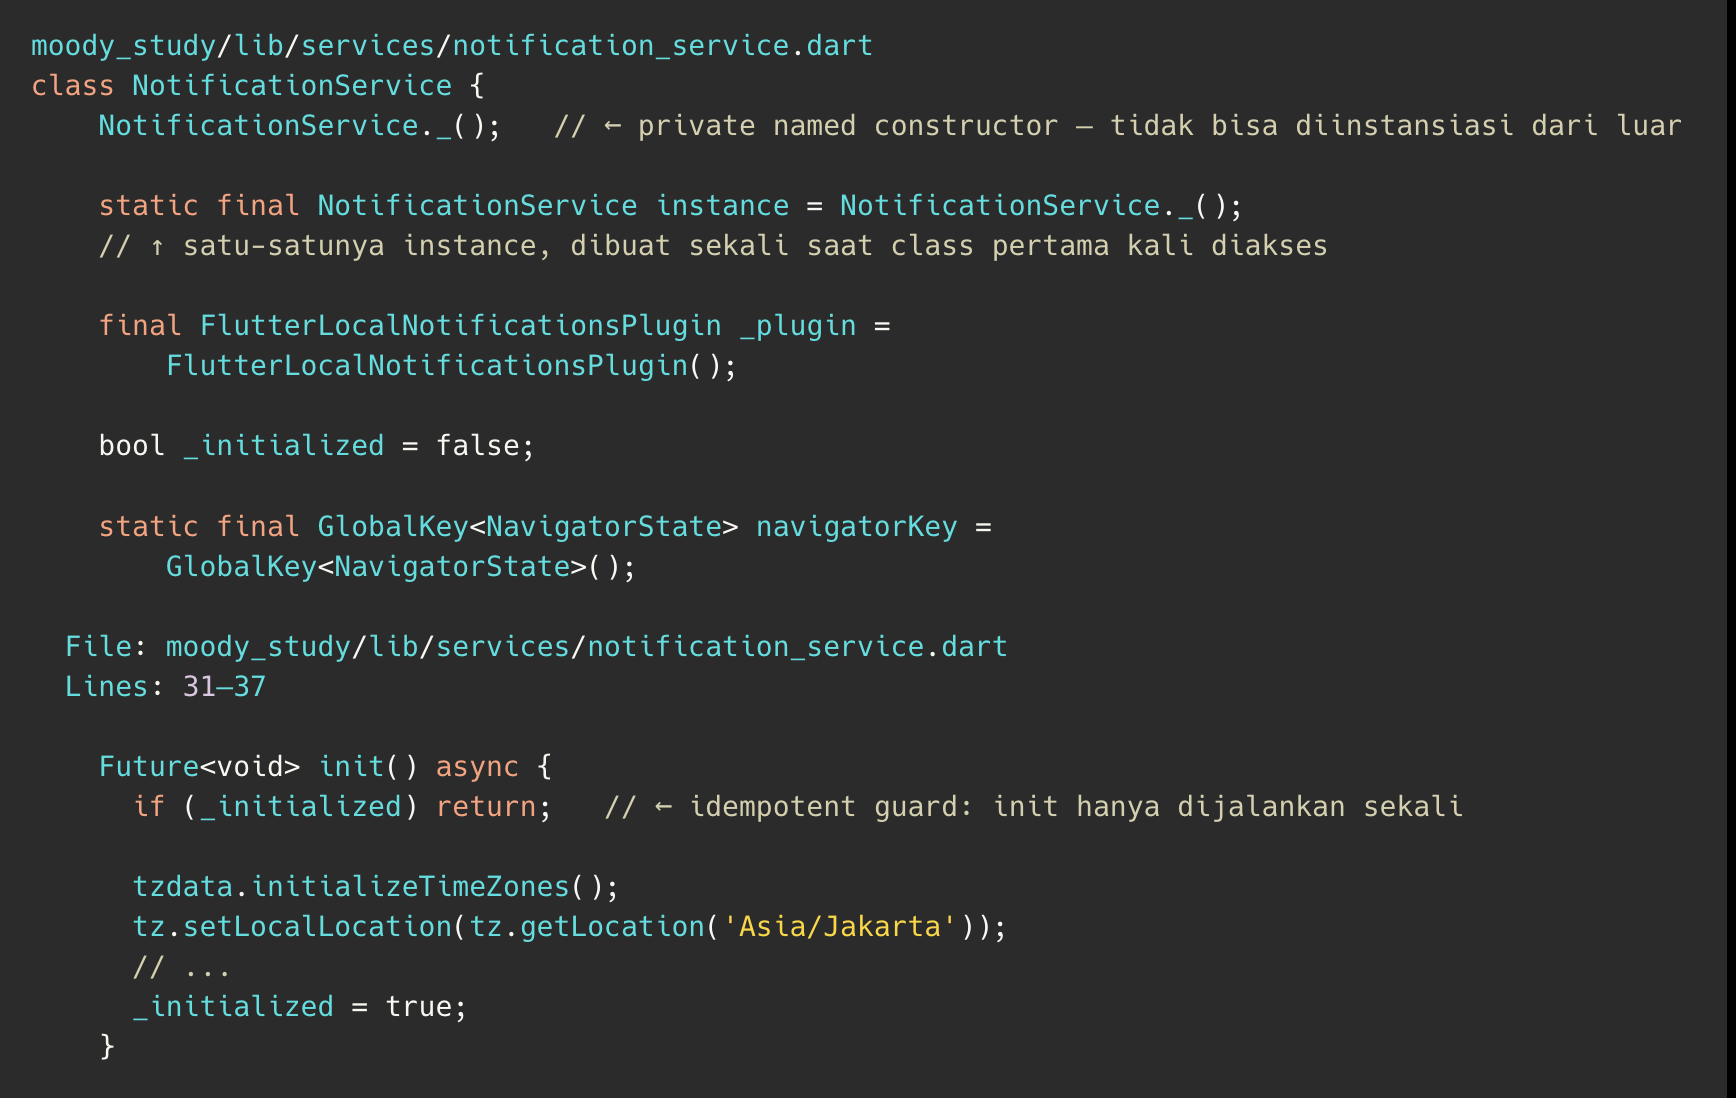
\includegraphics[width=\linewidth,height=0.23\textheight,keepaspectratio]{singleton1.png}
    \vspace{1ex}
\end{minipage} \\[2ex]
\hline

Singleton &
\begin{minipage}[t]{0.70\textwidth}
    \vspace{1ex}
    \centering
    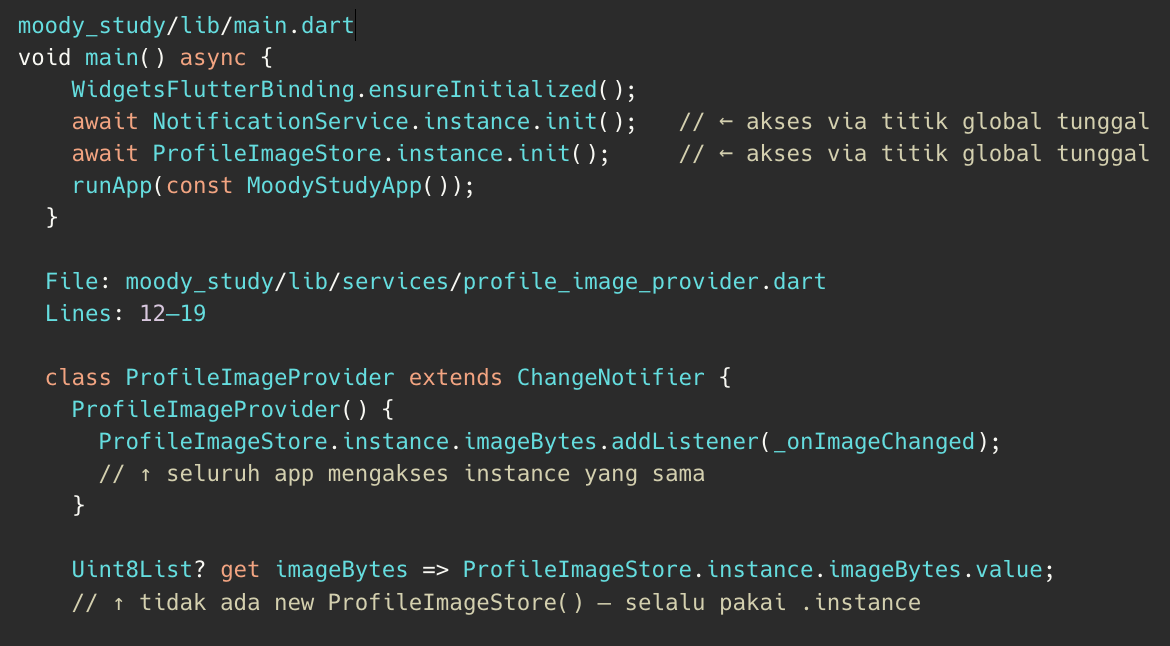
\includegraphics[width=\linewidth,height=0.23\textheight,keepaspectratio]{singleton2.png}
    \vspace{1ex}
\end{minipage} \\[2ex]
\hline

Singleton &
\begin{minipage}[t]{0.70\textwidth}
    \vspace{1ex}
    \centering
    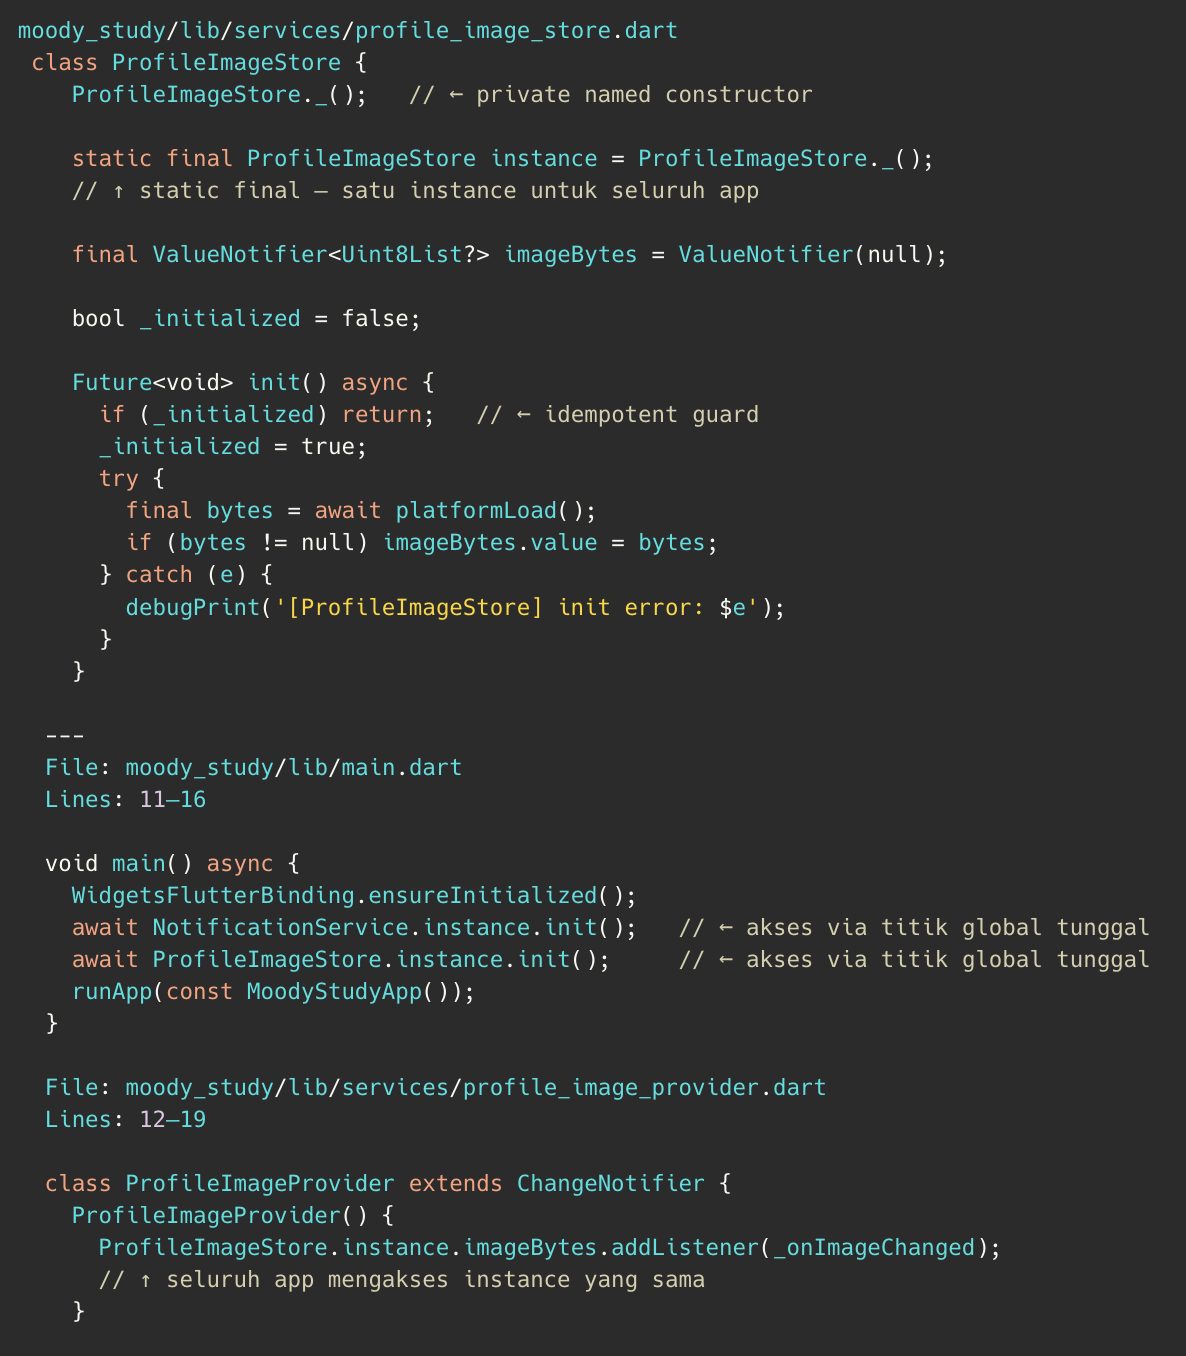
\includegraphics[width=\linewidth,height=0.23\textheight,keepaspectratio]{singleton3.png}
    \vspace{1ex}
\end{minipage} \\[2ex]
\hline

Adapter &
\begin{minipage}[t]{0.70\textwidth}
    \vspace{1ex}
    \centering
    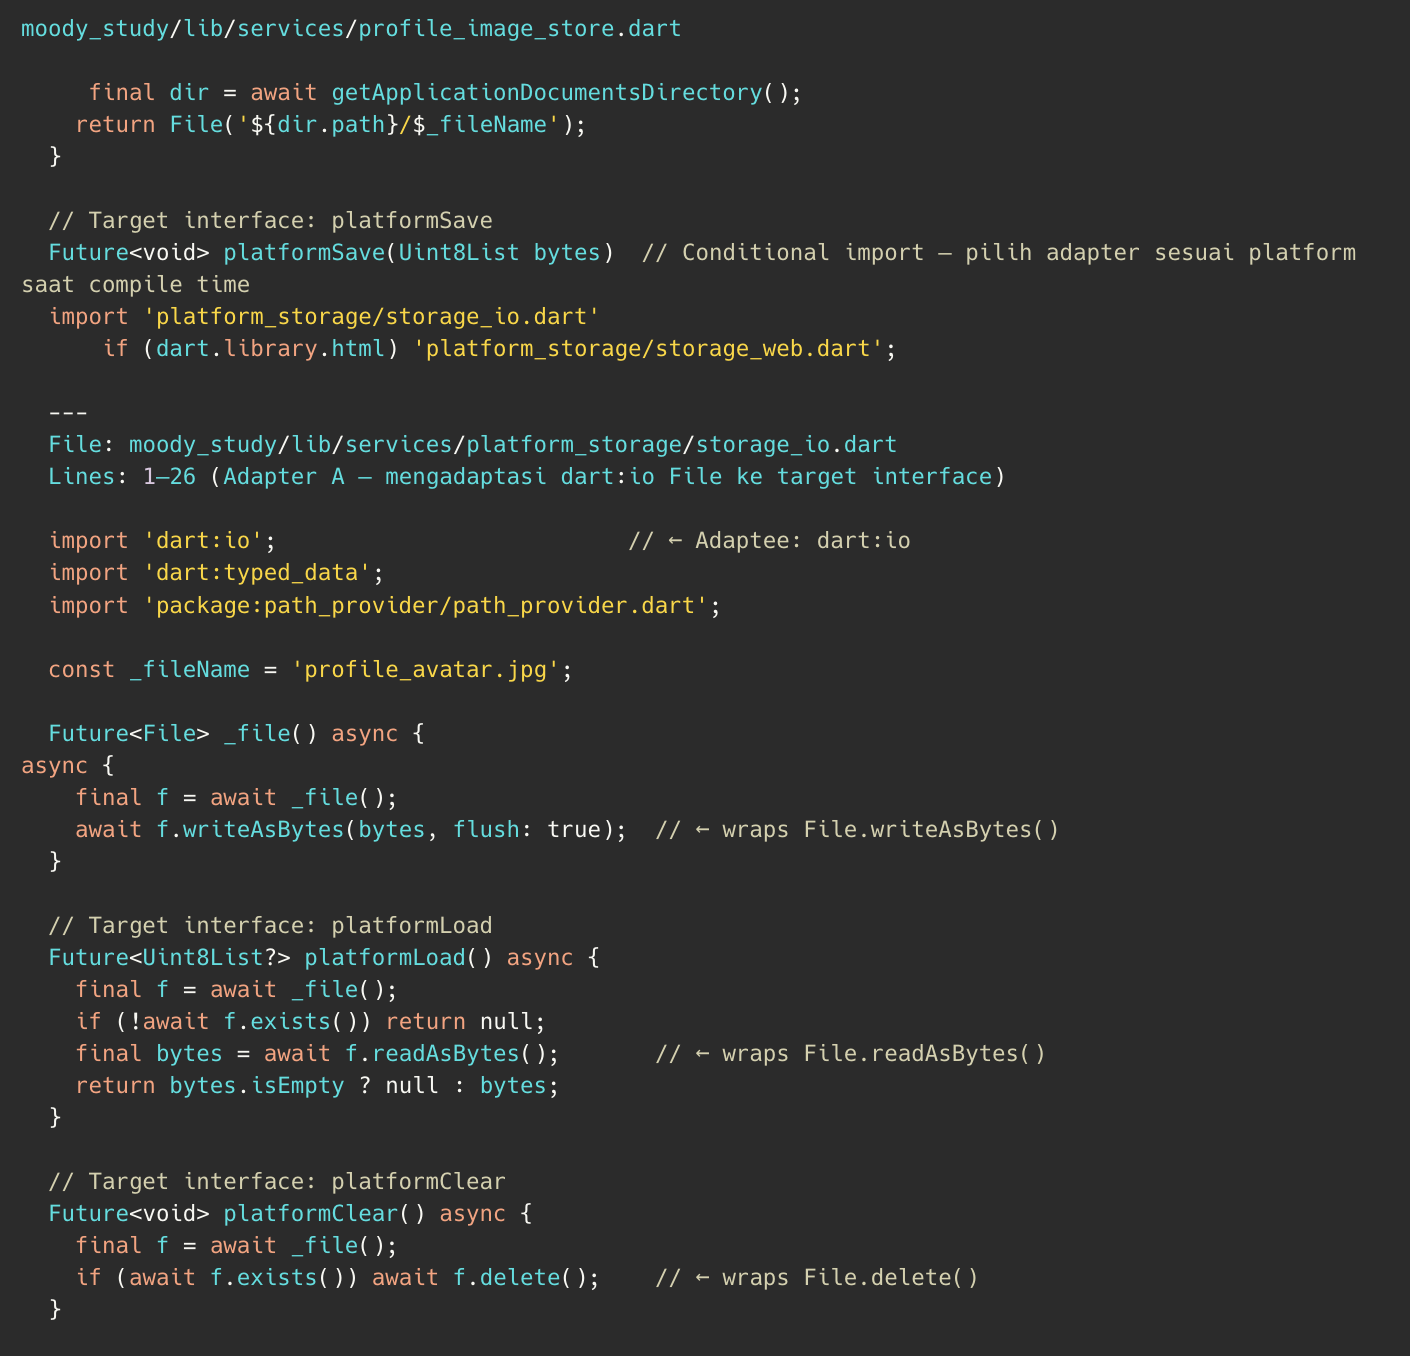
\includegraphics[width=\linewidth,height=0.23\textheight,keepaspectratio]{adapter1.png}
    \vspace{1ex}
\end{minipage} \\[2ex]
\hline

Adapter &
\begin{minipage}[t]{0.70\textwidth}
    \vspace{1ex}
    \centering
    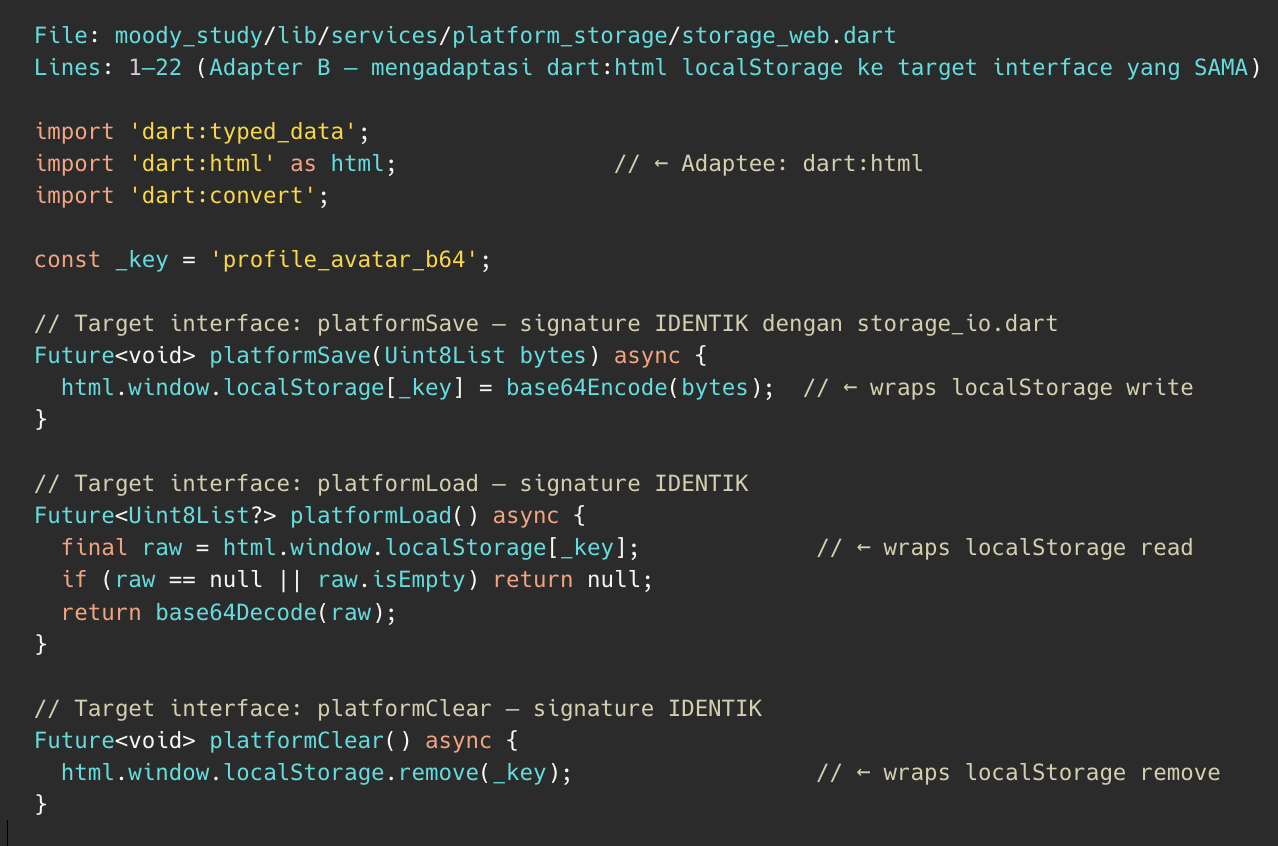
\includegraphics[width=\linewidth,height=0.23\textheight,keepaspectratio]{adapter2.png}
    \vspace{1ex}
\end{minipage} \\[2ex]
\hline

Adapter &
\begin{minipage}[t]{0.70\textwidth}
    \vspace{1ex}
    \centering
    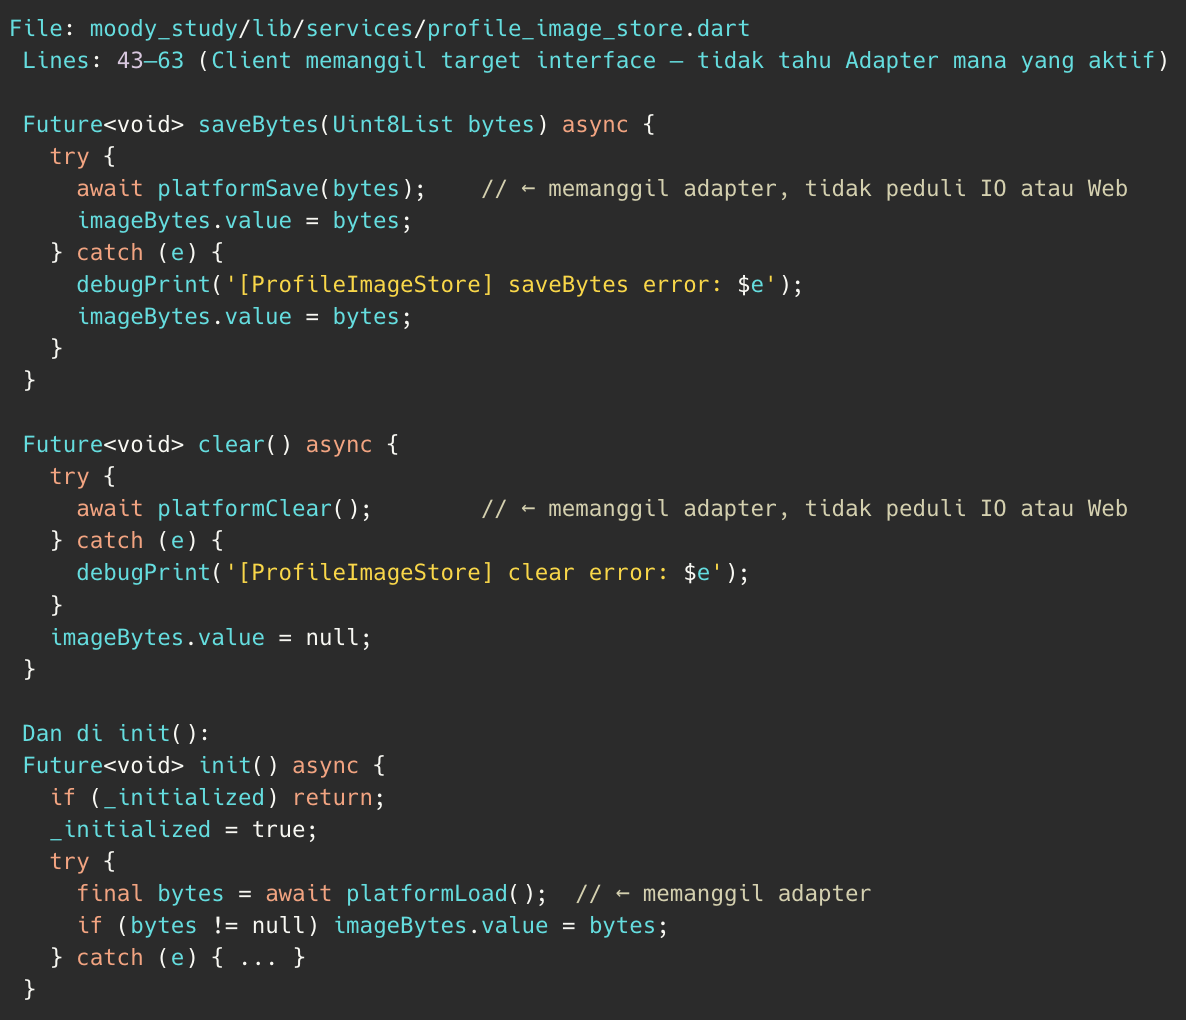
\includegraphics[width=\linewidth,height=0.23\textheight,keepaspectratio]{adapter3.png}
    \vspace{1ex}
\end{minipage} \\[2ex]
\hline

Observer &
\begin{minipage}[t]{0.70\textwidth}
    \vspace{1ex}
    \centering
    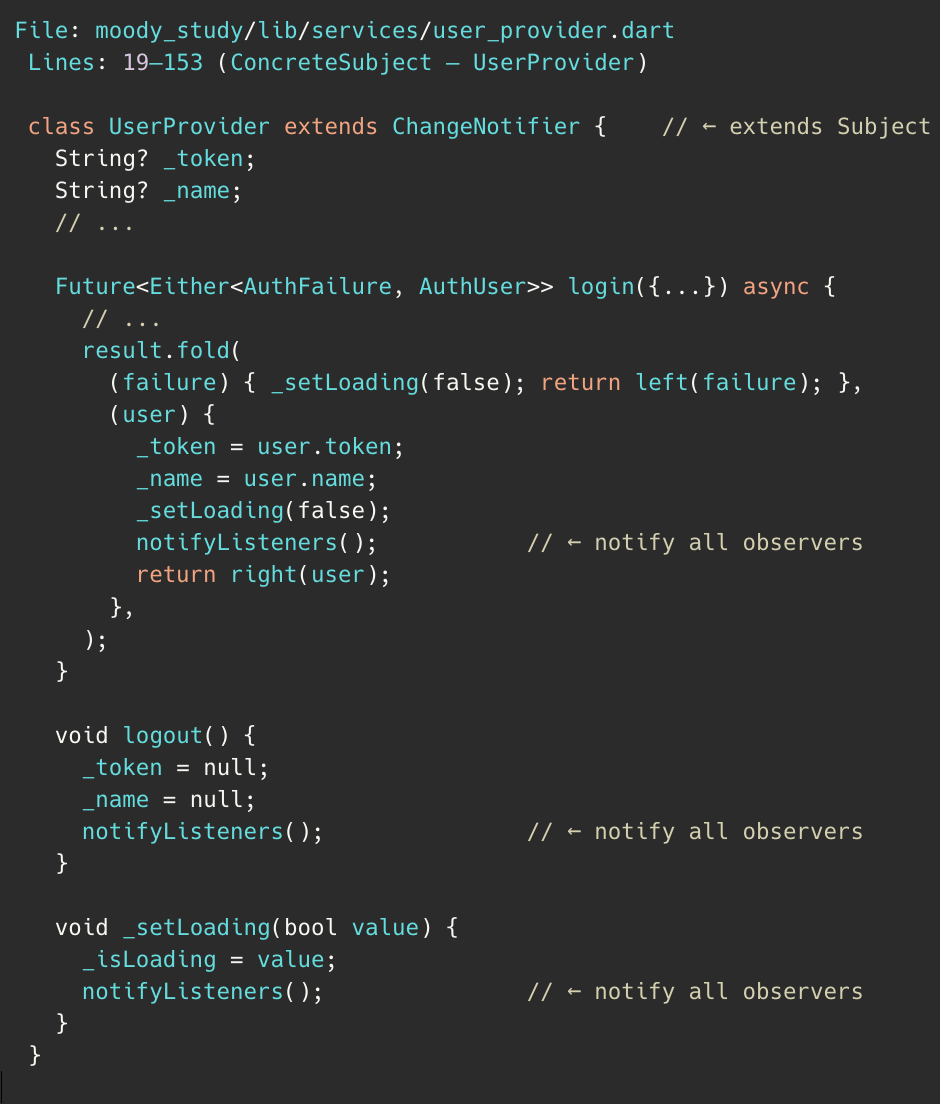
\includegraphics[width=\linewidth,height=0.23\textheight,keepaspectratio]{observer1.png}
    \vspace{1ex}
\end{minipage} \\[2ex]
\hline

Observer &
\begin{minipage}[t]{0.70\textwidth}
    \vspace{1ex}
    \centering
    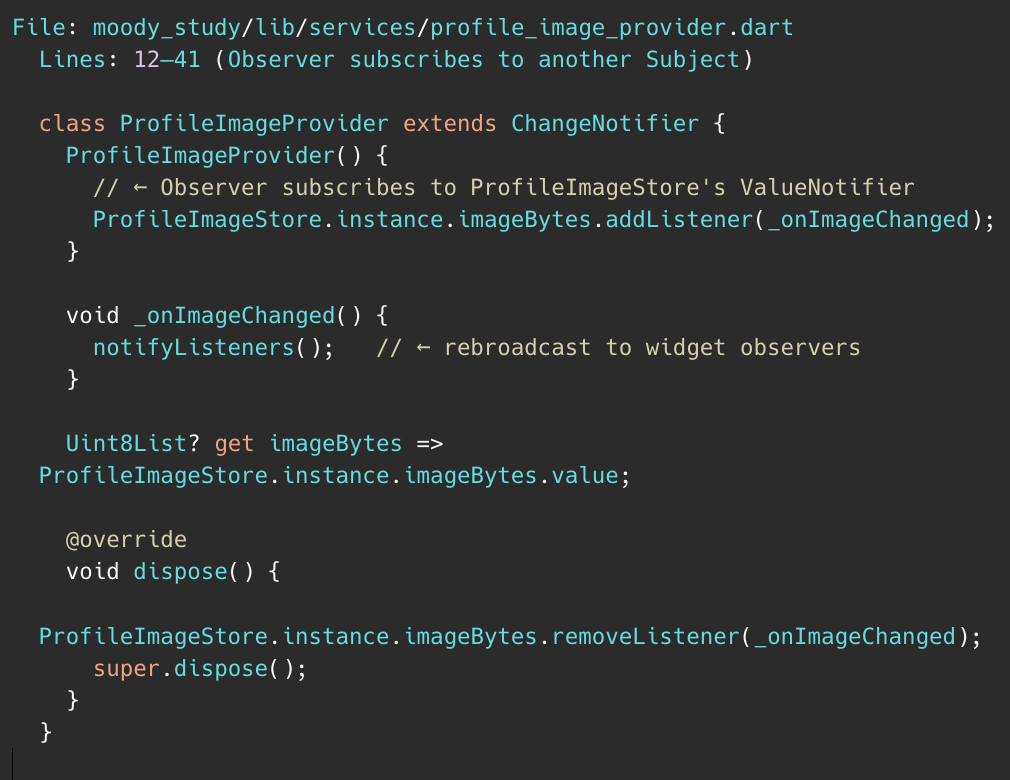
\includegraphics[width=\linewidth,height=0.23\textheight,keepaspectratio]{observer2.png}
    \vspace{1ex}
\end{minipage} \\[2ex]
\hline

Observer &
\begin{minipage}[t]{0.70\textwidth}
    \vspace{1ex}
    \centering
    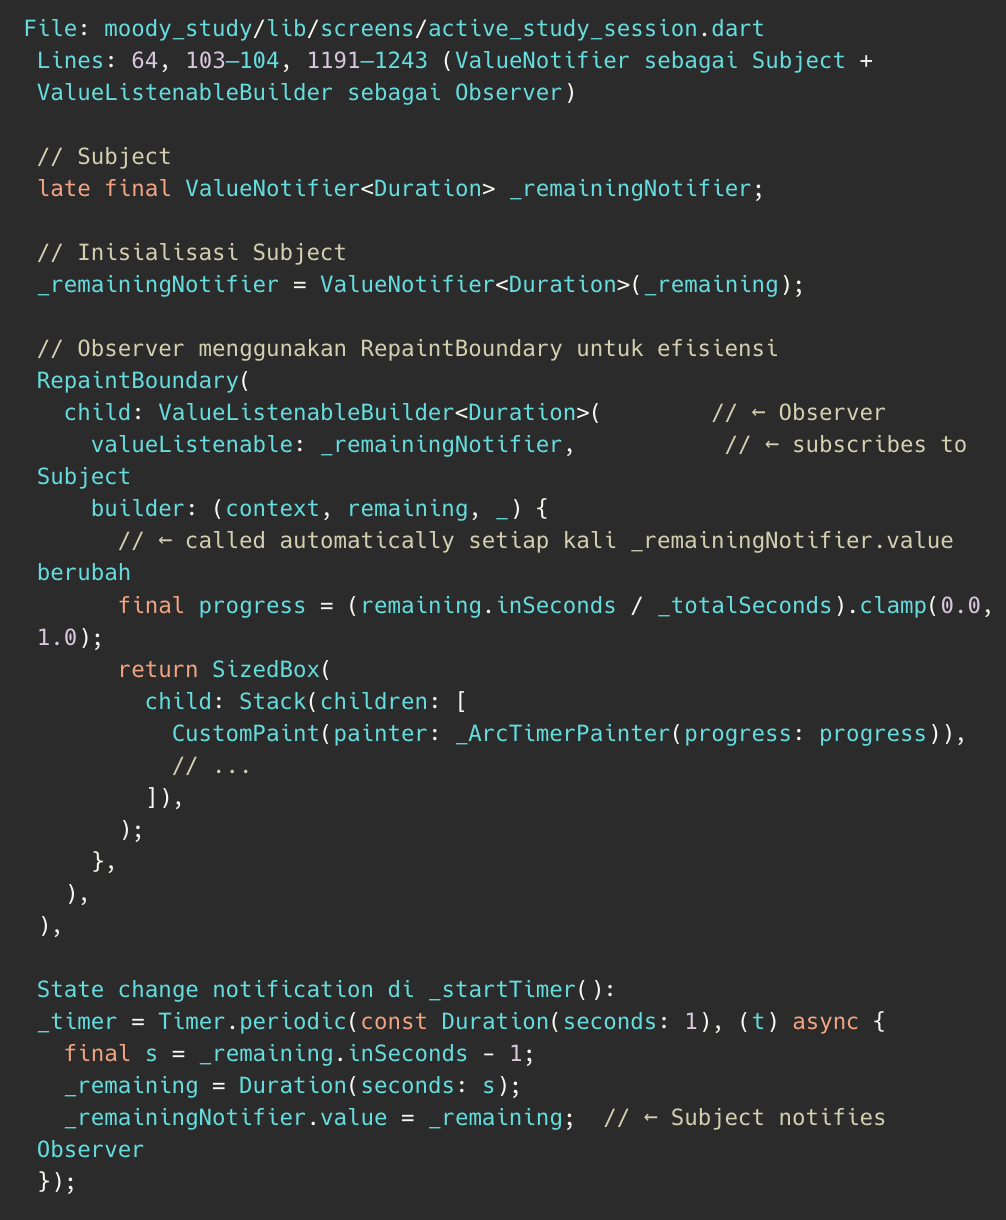
\includegraphics[width=\linewidth,height=0.23\textheight,keepaspectratio]{observer3.png}
    \vspace{1ex}
\end{minipage} \\[2ex]
\hline

Chain of Responsibility &
\begin{minipage}[t]{0.70\textwidth}
    \vspace{1ex}
    \centering
    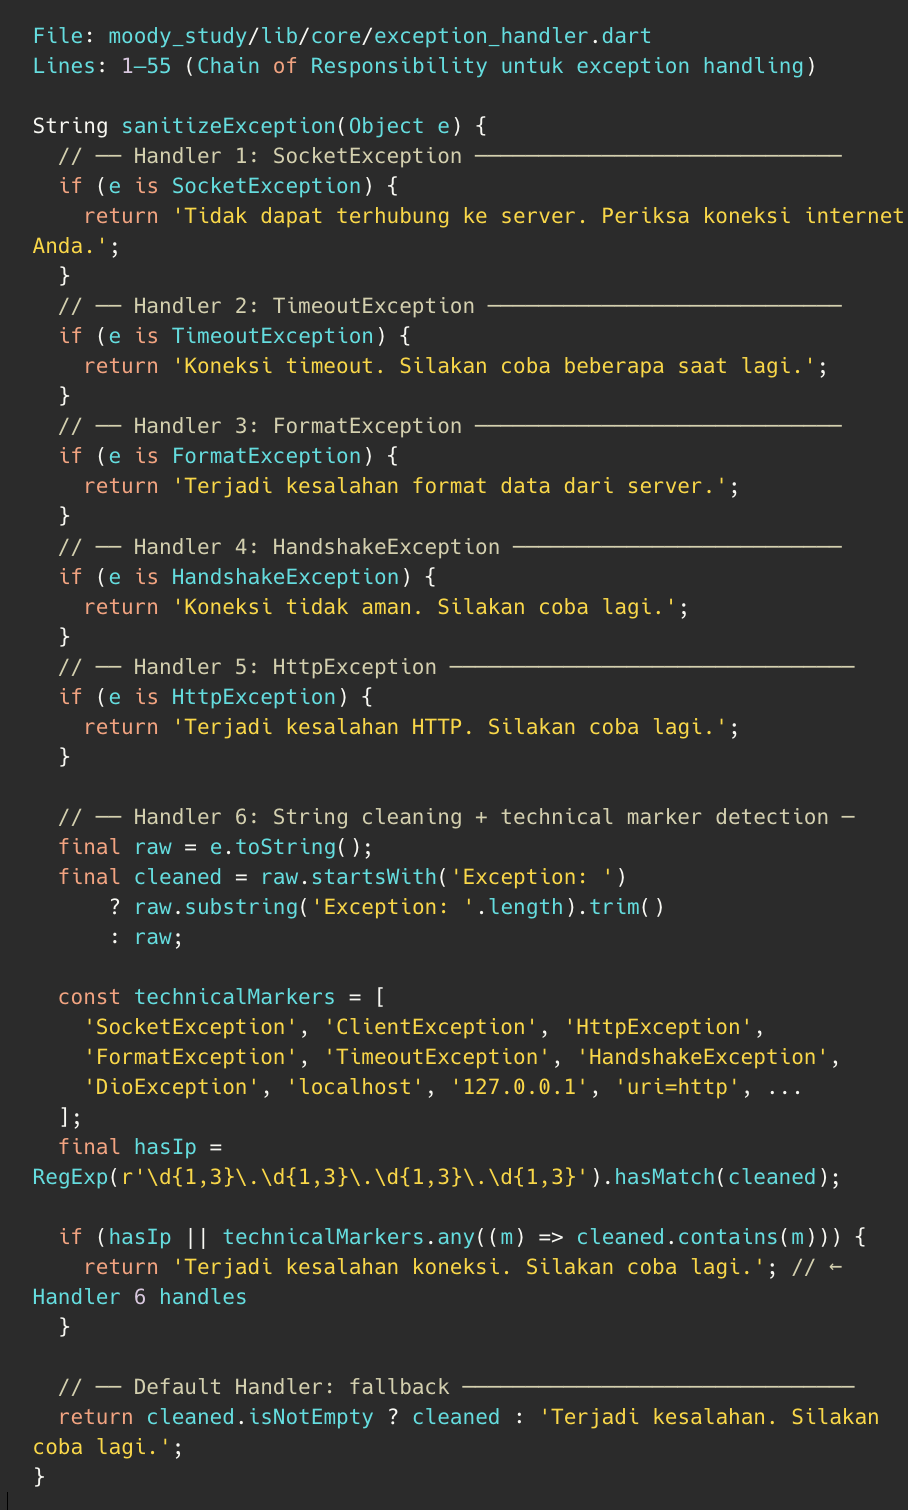
\includegraphics[width=\linewidth,height=0.23\textheight,keepaspectratio]{chain1.png}
    \vspace{1ex}
\end{minipage} \\[2ex]
\hline

Chain of Responsibility &
\begin{minipage}[t]{0.70\textwidth}
    \vspace{1ex}
    \centering
    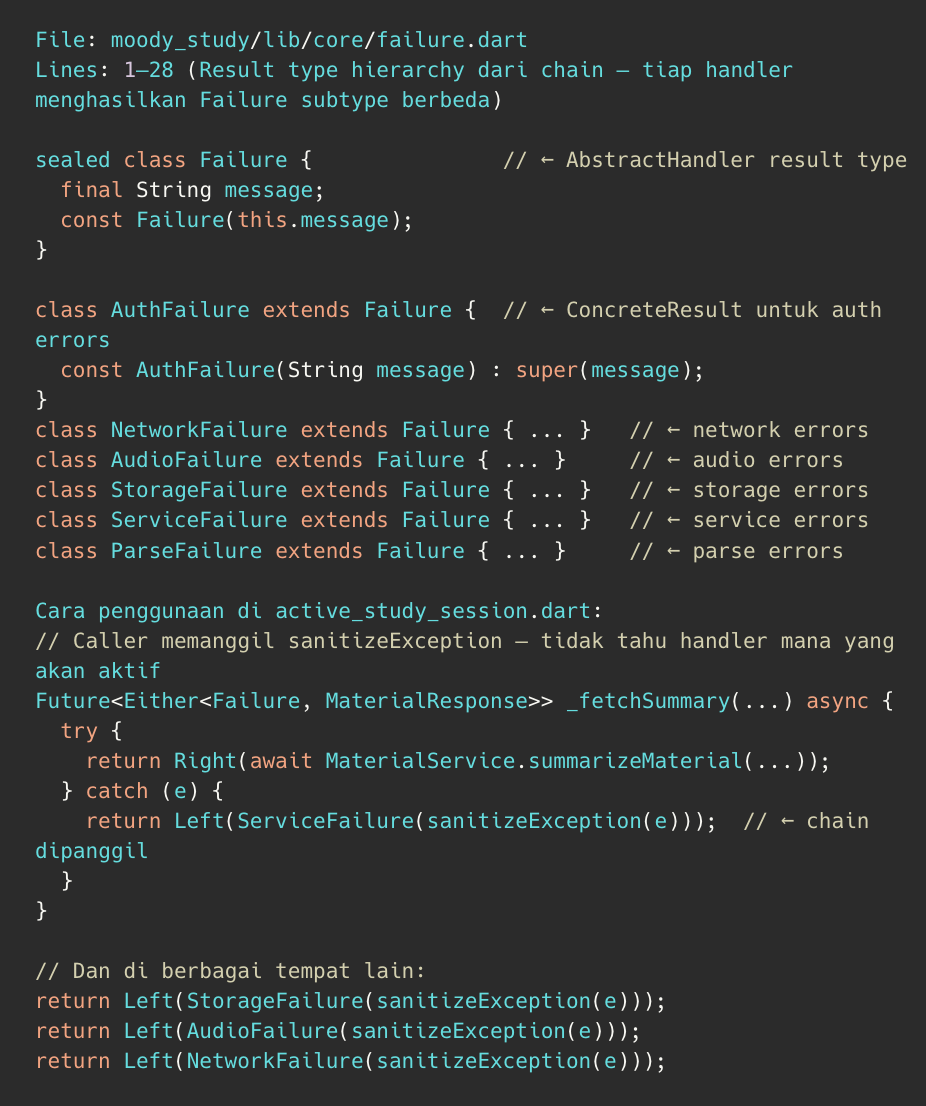
\includegraphics[width=\linewidth,height=0.23\textheight,keepaspectratio]{chain2.png}
    \vspace{1ex}
\end{minipage} \\[2ex]
\hline

Facade &
\begin{minipage}[t]{0.70\textwidth}
    \vspace{1ex}
    \centering
    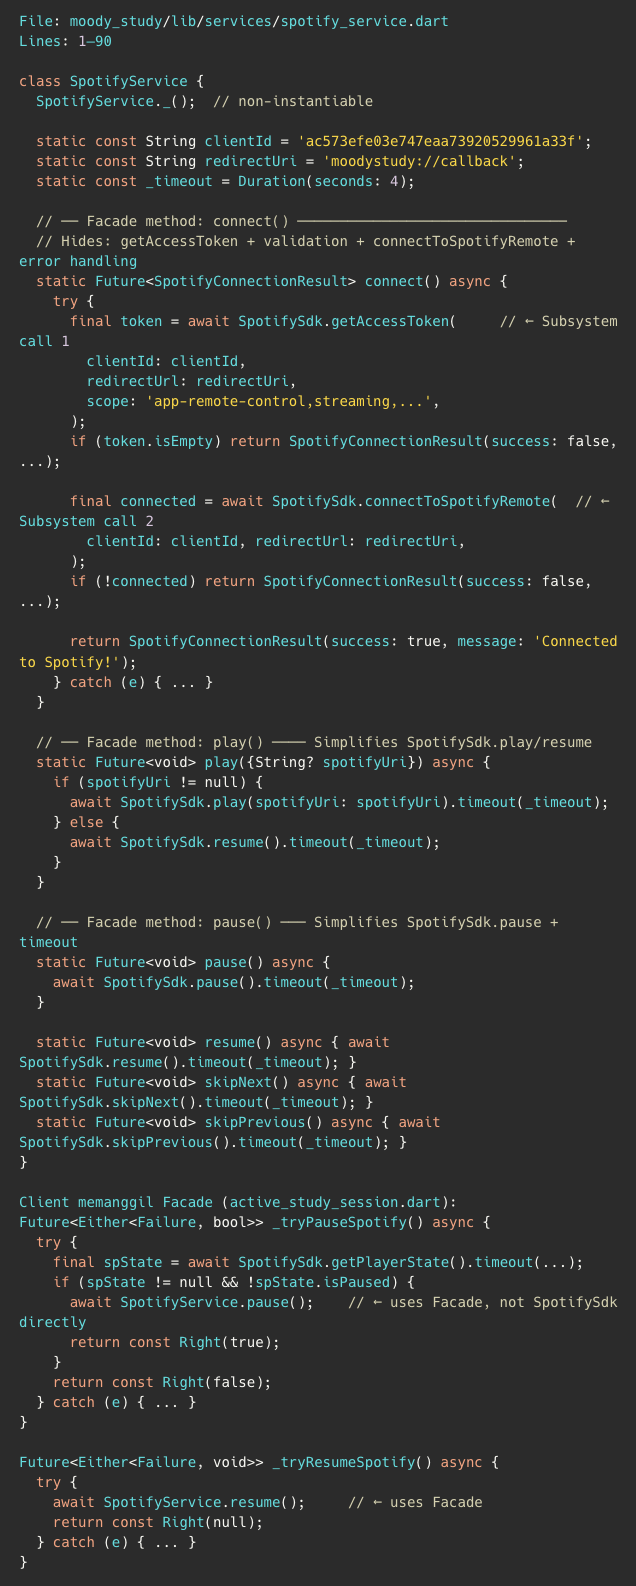
\includegraphics[width=\linewidth,height=0.23\textheight,keepaspectratio]{facade1.png}
    \vspace{1ex}
\end{minipage} \\[2ex]
\hline

\end{longtable}


Deviasi yang mungkin terjadi adalah perubahan nama kelas, penyesuaian endpoint, dan penyederhanaan alur AI berdasarkan kebutuhan implementasi. Setiap deviasi harus didokumentasikan dengan alasan teknis, seperti keterbatasan API, performa, keamanan, atau perubahan kebutuhan pengguna.

\section{System Architecture}

Arsitektur sistem menggunakan Flutter Clean Architecture pada sisi frontend dan layered architecture pada sisi backend Spring Boot. Flutter dibagi menjadi presentation layer, state management layer menggunakan Riverpod, domain layer, dan data layer. Spring Boot dibagi menjadi controller layer, service layer, repository layer, security layer, dan persistence layer.

Alur komunikasi sistem dimulai dari Flutter Client yang mengirim request JSON melalui REST API. Spring Boot menerima request melalui controller, memproses logika pada service layer, mengakses database PostgreSQL melalui repository dan ORM, lalu mengembalikan response JSON ke aplikasi Flutter.

\section{API Contract}

API Contract mendefinisikan komunikasi antara Flutter dan Spring Boot menggunakan REST API dengan format JSON. Dokumentasi lengkap dapat dikembangkan menggunakan OpenAPI/Swagger.

\begin{center}
\renewcommand{\arraystretch}{1.3}
\begin{tabular}{|p{0.18\textwidth}|p{0.24\textwidth}|p{0.42\textwidth}|}
\hline
\textbf{Method} & \textbf{Endpoint} & \textbf{Fungsi} \\
\hline
POST & /api/auth/register & Registrasi pengguna baru. \\
\hline
POST & /api/auth/login & Autentikasi pengguna dan menghasilkan JWT. \\
\hline
POST & /api/materials/upload & Mengunggah materi belajar. \\
\hline
POST & /api/ai/summary & Menghasilkan ringkasan materi. \\
\hline
POST & /api/ai/quiz & Menghasilkan latihan soal. \\
\hline
POST & /api/schedules & Membuat jadwal belajar manual atau otomatis. \\
\hline
GET & /api/statistics & Mengambil statistik belajar pengguna. \\
\hline
\end{tabular}
\end{center}

Contoh request login berisi email dan password, sedangkan response mengembalikan token JWT, data pengguna, dan role. Contoh response statistik berisi total sesi, waktu aktif, waktu distraksi, streak, level, dan rekomendasi AI.


\section{Flutter Implementation}

Bagian ini menjelaskan implementasi sisi frontend dari aplikasi Moody Study yang dikembangkan menggunakan Flutter. Implementasi Flutter berperan sebagai antarmuka utama pengguna untuk menjalankan proses belajar, mulai dari autentikasi, pemilihan mood, pengaturan sesi belajar, penjadwalan, pemutaran musik, pemantauan fokus, hingga visualisasi statistik dan gamifikasi. Seluruh fitur frontend dirancang agar terhubung dengan backend Spring Boot melalui REST API, sehingga data pengguna, materi, jadwal, quest, streak, dan statistik dapat diproses secara terpusat namun tetap ditampilkan secara interaktif di aplikasi.

\subsection{Key Features}

Aplikasi Moody Study dibangun dengan Flutter dan mencakup sejumlah fitur utama yang mendukung pengalaman belajar berbasis suasana hati atau mood-based learning.

\paragraph{Autentikasi Pengguna}

Aplikasi menyediakan alur registrasi dan login lengkap melalui \texttt{AuthService} yang berkomunikasi dengan backend REST API menggunakan endpoint \texttt{/api/auth/register} dan \texttt{/api/auth/login}. Token JWT yang diterima dari server disimpan secara statis di \texttt{AuthService.token} dan disertakan pada setiap permintaan API berikutnya sebagai Bearer token di header Authorization.

\paragraph{Sesi Belajar Aktif}

Fitur inti aplikasi adalah \texttt{ActiveStudySession}, yaitu screen yang mengelola sesi belajar dengan timer countdown yang dapat di-pause dan dilanjutkan. Pengguna dapat mengunggah materi seperti PDF atau file lain, yang kemudian diproses secara otomatis untuk menghasilkan ringkasan menggunakan layanan backend melalui \texttt{MaterialService}. Selama sesi berlangsung, aplikasi memantau apakah pengguna meninggalkan layar atau away detection menggunakan \texttt{WidgetsBindingObserver}\linebreak[1].

\paragraph{Penjadwalan dengan AI (Asisten Oddy)}

\texttt{ScheduleScreen} memiliki mode manual dan mode AI bernama Asisten Oddy. Pada mode AI, pengguna memasukkan daftar mata pelajaran satu per satu, secara massal, atau melalui file upload, memilih hari-hari yang tersedia, rentang jam belajar, dan durasi sesi. Sistem kemudian memanggil \texttt{ScheduleService.generateAutoSchedule()}\linebreak[1] untuk menghasilkan jadwal secara otomatis yang dapat diedit sebelum disimpan.

\paragraph{Sistem Gamifikasi}

Aplikasi menerapkan mekanisme gamifikasi yang terdiri dari sistem Coins atau experience points, streak harian, level pengguna, dan nyawa atau life. Setiap akhir sesi belajar, sistem mengecek perubahan streak dan level melalui \texttt{StreakService}, lalu menampilkan layar animasi \texttt{LevelUpScreen} atau \texttt{StreakCounterScreen} apabila ada pencapaian baru. Jika pengguna kehilangan nyawa, sistem menampilkan \texttt{LifeLostPopup}.

\paragraph{Daily Quest}

Layar \texttt{DailyQuestScreen} menampilkan tiga quest harian yang harus diselesaikan beserta total Coins yang telah dikumpulkan pada hari tersebut. Data diambil dari endpoint \texttt{/api/quest/daily} melalui \texttt{DailyQuestService}.

\paragraph{Integrasi Spotify}

Aplikasi mengintegrasikan Spotify SDK melalui \texttt{SpotifyService} yang memungkinkan pengguna menghubungkan akun Spotify untuk memutar, menjeda, melanjutkan, dan berpindah lagu langsung dari dalam aplikasi tanpa meninggalkan sesi belajar.

\paragraph{Notifikasi Terjadwal}

\texttt{NotificationService} menggunakan package \texttt{flutter\_local\_notifications} dengan dukungan timezone \texttt{Asia/Jakarta} untuk mengirimkan notifikasi pengingat jadwal belajar. Notifikasi membawa payload JSON berisi informasi subjek, mood, dan lokasi, sehingga ketika pengguna mengetuk notifikasi, aplikasi langsung membuka layar sesi belajar yang relevan.

\paragraph{Statistik dan Awards}

\texttt{StatistikScreen} mengagregasi data dari beberapa endpoint API secara paralel, yaitu \texttt{/api/stats}, \texttt{/api/streak}, \texttt{/api/award}, dan \texttt{/api/quest/daily}, menggunakan \texttt{Future.wait}. Data tersebut ditampilkan sebagai statistik lengkap seperti total sesi, total menit belajar, focus rate, sesi per hari, mood favorit, lokasi favorit, level, serta daftar penghargaan yang telah diraih.

\paragraph{Internasionalisasi}

Seluruh teks antarmuka pengguna mendukung dua bahasa, yaitu Bahasa Indonesia dan Bahasa Inggris, melalui kelas \texttt{AppLocalizations}.

\subsection{State Management Flow}

Aplikasi menggunakan Provider sebagai solusi state management utama, dengan tiga \texttt{ChangeNotifier} yang didaftarkan di level root \texttt{MaterialApp} menggunakan \texttt{MultiProvider}.

\paragraph{LanguageProvider}

\texttt{LanguageProvider} menyimpan state bahasa aktif, yaitu \texttt{AppLanguage.id} atau \texttt{AppLanguage.en}. Widget yang membutuhkan terjemahan mengakses \texttt{AppLocalizations.of(context)} yang secara internal memanggil \texttt{context.watch<LanguageProvider>()}, sehingga seluruh UI otomatis diperbarui saat bahasa diganti.

\paragraph{UserProvider}

\texttt{UserProvider} menyimpan state autentikasi pengguna, seperti token JWT, username, nama lengkap, email, status loading, dan pesan error. Method \texttt{login()} dan \texttt{register()} memanggil \texttt{AuthService}, lalu memperbarui state dan memanggil \texttt{notifyListeners()} setelah mendapat respons dari server. Method \texttt{logout()} membersihkan semua data state sekaligus memanggil \texttt{AuthService.logout()}. Tersedia pula method utilitas seperti \texttt{updateUsername()}, \texttt{updateName()}, \texttt{updateToken()}, dan \texttt{refreshUserInfo()} untuk sinkronisasi data dengan server setelah operasi profil.

\paragraph{ProfileImageProvider}

\texttt{ProfileImageProvider} merupakan wrapper \texttt{ChangeNotifier} di atas \texttt{ProfileImageStore} yang menggunakan pola singleton. Provider ini mendengarkan \texttt{ValueNotifier<Uint8List?>} dari store menggunakan \texttt{addListener}, kemudian meneruskan perubahan ke widget tree melalui \texttt{notifyListeners()}. Pola ini memisahkan logika persistensi atau store dari logika reaktivitas UI atau provider.

Untuk state lokal yang bersifat screen-specific, seperti data jadwal, progress timer, dan loading state API, aplikasi menggunakan \texttt{StatefulWidget} dengan \texttt{setState()} secara langsung tanpa Provider.

\subsection{Custom Widgets}

\paragraph{MoodyTitle}

\texttt{MoodyTitle} adalah widget animasi intro yang mereplikasi animasi judul Moody Study. Widget ini menggunakan \texttt{TickerProviderStateMixin}\linebreak[1] untuk mengelola tujuh \texttt{AnimationController}\linebreak[1] secara bersamaan: empat controller untuk kemunculan tiap titik dengan bounce masuk menggunakan \texttt{Curves.elasticOut}, satu controller untuk keruntuhan jarak antar titik atau gap collapse, empat controller untuk transformasi titik menjadi teks atau morph, dan satu controller untuk animasi mengambang atau idle float yang berjalan secara looping. Urutan animasi dijalankan secara sekuensial menggunakan \texttt{async/await} dengan \texttt{Future.delayed} di dalam method \texttt{\_runSequence()}. Ukuran titik dan font bersifat responsif terhadap lebar layar menggunakan perhitungan \texttt{MediaQuery} dengan nilai clamp.

\paragraph{MusicVisualizerWidget}

\texttt{MusicVisualizerWidget} adalah widget floating yang menampilkan visualisasi musik berupa empat batang animasi atau audio bars. Batang-batang tersebut bergerak menggunakan fungsi sinus dengan frekuensi dan fase berbeda, yaitu \texttt{\_barFreq} dan \texttt{\_barPhase}, yang dianimasikan oleh \texttt{AnimationController}\linebreak[1] secara looping selama 10 detik. Widget ini memiliki dua animasi terpisah: animasi masuk berupa fade dan slide dari bawah, serta animasi bar yang terus berjalan. Ketika musik di-pause, batang-batang secara otomatis menyusut ke ukuran minimum menggunakan \texttt{AnimatedContainer}.

\paragraph{NowPlayingWidget}

\texttt{NowPlayingWidget} adalah widget positioned di bagian atas layar yang menampilkan informasi lagu yang sedang diputar. Widget ini menggunakan animasi slide masuk dari atas dengan spring curve \texttt{Cubic(0.34, 1.56, 0.64, 1)}, ikon musik yang memantul atau note bounce, dan titik-titik berkedip melalui \texttt{\_BlinkingDots} sebagai indikator bahwa lagu sedang diputar. Warna aksen widget berubah antara hijau dan abu-abu tergantung status pemutaran musik.

\paragraph{DailyQuestScreen}

\texttt{DailyQuestScreen} adalah widget yang menampilkan kartu-kartu quest harian berikut progress bar untuk setiap quest. Widget ini memanggil \texttt{DailyQuestService.getDailyQuests()}\linebreak[1] saat inisialisasi dan menangani tiga state utama, yaitu loading, error, dan data tersedia.

\subsection{Advanced Features}

Bagian advanced features mengacu pada fitur lanjutan Flutter yang benar-benar ada pada implementasi Moody Study. Dari kategori yang diminta pada spesifikasi proyek, aplikasi ini menggunakan beberapa fitur berikut.

\begin{center}
\renewcommand{\arraystretch}{1.2}
\resizebox{\textwidth}{!}{%
\begin{tabular}{|p{0.36\textwidth}|p{0.46\textwidth}|p{0.12\textwidth}|}
\hline
\textbf{Advanced Feature Category} & \textbf{Implementation in Moody Study} & \textbf{Status} \\
\hline
Push notifications / scheduled notifications & \texttt{NotificationService} menggunakan \texttt{flutter\_local\_notifications} untuk reminder jadwal belajar dengan payload JSON dan deep link ke sesi belajar. & Implemented \\
\hline
Animated transitions using custom route / animation widgets & \texttt{LevelUpScreen}, \texttt{StreakCounterScreen}, \texttt{LifeLostPopup}, \texttt{MusicVisualizer}, dan \texttt{NowPlayingWidget} menggunakan animasi transisi, fade, slide, bounce, progress, dan visualizer. & Implemented \\
\hline
Internationalization (i18n) with at least 2 languages & Aplikasi mendukung Bahasa Indonesia dan Bahasa Inggris melalui \texttt{AppLocalizations}, \texttt{LanguageProvider}, dan pilihan \texttt{AppLanguage.id}/\texttt{AppLanguage.en}. & Implemented \\
\hline
\end{tabular}%
}
\end{center}

Dengan demikian, aplikasi memenuhi syarat advanced features karena sudah mencakup minimal dua kategori yang benar-benar diimplementasikan, yaitu animated transitions dan internationalization, serta didukung oleh fitur notifikasi terjadwal.

\paragraph{Away Detection dan Focus Monitoring}

\texttt{ActiveStudySession} mengimplementasikan \texttt{WidgetsBindingObserver}\linebreak[1] untuk mendeteksi ketika pengguna meninggalkan aplikasi. Ketika \texttt{AppLifecycleState} berpindah ke \texttt{paused} atau \texttt{inactive}, sebuah \texttt{Timer} selama 30 detik dimulai. Jika pengguna tidak kembali dalam batas waktu tersebut, alarm dibunyikan menggunakan \texttt{AudioPlayer} dengan loop aktif, layar memancarkan kilat merah secara periodik menggunakan \texttt{FlashTimer}, dan perangkat bergetar menggunakan package \texttt{vibration}. Total durasi distraksi dicatat di \texttt{\_totalDistractionSeconds} dan digunakan untuk menghitung focus rate sesi.

\paragraph{AI Schedule Generation}

Jadwal belajar dapat dibuat secara otomatis oleh AI melalui \texttt{ScheduleService.generateAutoSchedule()}\linebreak[1]. Pengguna dapat memberikan input berupa daftar mata pelajaran, hari-hari yang tersedia, rentang jam belajar, durasi per sesi, dan jumlah hari ke depan. Selain input teks, pengguna juga dapat mengunggah file, termasuk PDF dan DOCX, yang kontennya diekstrak untuk dijadikan konteks input AI. Hasil jadwal yang dihasilkan AI dapat diedit secara inline sebelum disimpan ke database.

\paragraph{Cross-Platform Profile Image Storage}

Penyimpanan foto profil menggunakan conditional import Dart untuk memberikan implementasi yang berbeda di setiap platform tanpa mengubah antarmuka publik. Di web, foto disimpan sebagai string Base64 di \texttt{window.localStorage} melalui \texttt{dart:html}. Di mobile dan desktop, foto disimpan sebagai file biner di application documents directory menggunakan \texttt{path\_provider}. Kedua implementasi mengekspos tiga fungsi yang identik, yaitu \texttt{platformSave()}, \texttt{platformLoad()}, dan \texttt{platformClear()}.

\paragraph{PDF Generation dan Flashcard}

Di akhir sesi belajar, pengguna dapat menyimpan ringkasan materi sebagai file PDF yang digenerate secara lokal menggunakan package \texttt{pdf}. Materi yang diunggah selama sesi juga dapat diproses untuk menghasilkan flashcard melalui layar \texttt{OddyFlashcardScreen}\linebreak[1]. Ekstraksi teks dari file PDF yang diunggah dilakukan menggunakan package \texttt{flutter\_pdf\_text}.

\paragraph{Notifikasi Deep Link}

Sistem notifikasi mendukung deep linking berbasis payload JSON. Ketika notifikasi jadwal belajar diketuk, baik saat aplikasi aktif, di background, maupun dalam kondisi terminated, aplikasi mem-parse payload untuk mendapatkan konteks sesi seperti subjek, mood, dan lokasi, lalu langsung menavigasi pengguna ke layar sesi belajar yang sesuai. Navigasi dilakukan melalui \texttt{GlobalKey<NavigatorState>} yang dapat diakses dari luar widget tree.

\paragraph{Gamifikasi End-of-Session}

Setelah setiap sesi belajar selesai, sistem secara otomatis mengecek perubahan data streak dan level dengan membandingkan nilai sebelum dan sesudah sesi. Terdapat tiga kemungkinan animasi yang dapat muncul: \texttt{LevelUpScreen} jika pengguna naik level, \texttt{StreakCounterScreen} jika streak meningkat, dan \texttt{LifeLostPopup} jika pengguna kehilangan nyawa akibat sering tidak fokus. Layar-layar ini diimplementasikan sebagai page route khusus dengan transisi animasi tersendiri.

\section{Spring Boot Implementation}

Implementasi Spring Boot berfokus pada REST API, keamanan, logika bisnis, dan persistence. Service layer menangani proses autentikasi, manajemen materi, ringkasan AI, generate latihan soal, penjadwalan belajar, statistik, dan gamifikasi. Security config menggunakan Spring Security dan JWT untuk melindungi endpoint.

Database menggunakan PostgreSQL dengan ORM Spring Data JPA/Hibernate. Skema database mencakup tabel User, Material, Summary, Flashcard, Quiz, StudySchedule, StudySession, MoodLog, Statistic, Quest, Streak, dan Life. Flyway migrations dapat digunakan untuk menjaga perubahan skema database secara terkontrol.


\section{Flutter Testing \& Benchmarking}

Bagian ini menjelaskan proses pengujian dan benchmarking pada aplikasi Flutter Moody Study. Pengujian dilakukan untuk memastikan fitur utama berjalan sesuai kebutuhan, komponen UI dapat dirender dengan benar, alur end-to-end dapat terhubung dengan live Spring Boot API, serta performa aplikasi tetap stabil pada perangkat Android fisik.

\subsection{Functional Testing}

Functional testing dibagi menjadi unit testing, widget testing, dan integration testing. Ringkasan target pengujian ditunjukkan pada tabel berikut.

\begin{center}
\renewcommand{\arraystretch}{1.3}
\resizebox{\textwidth}{!}{%
\begin{tabular}{|p{0.22\textwidth}|p{0.22\textwidth}|p{0.43\textwidth}|}
\hline
\textbf{Type} & \textbf{Tool} & \textbf{Minimum Target} \\
\hline
Unit Testing & \texttt{flutter\_test} & Semua use case dan repository implementation diuji. \\
\hline
Widget Testing & \texttt{flutter\_test} & Minimal 5 core UI components diuji. \\
\hline
Integration Testing & \texttt{integration\_test} & Minimal 3 end-to-end flows terhadap live Spring Boot API. \\
\hline
\end{tabular}%
}
\end{center}

\subsection{Unit Testing}

\subsubsection{auth\_services\_test.dart}

Durasi pengujian adalah 00:10 dengan hasil +9 passed. Seluruh test utama berhasil dijalankan.

\begin{center}
\renewcommand{\arraystretch}{1.2}
\resizebox{\textwidth}{!}{%
\begin{tabular}{|p{0.08\textwidth}|p{0.68\textwidth}|p{0.14\textwidth}|}
\hline
\textbf{No.} & \textbf{Test Case} & \textbf{Status} \\
\hline
1 & \texttt{AuthService.register} melakukan parsing token dari response. & Pass \\
\hline
2 & \texttt{AuthService.register} melempar \texttt{AuthException} saat gagal. & Pass \\
\hline
3 & \texttt{AuthService.login} menyimpan token. & Pass \\
\hline
4 & \texttt{AuthService.login} gagal 401 dan menghasilkan exception. & Pass \\
\hline
5 & \texttt{AuthService.logout} membuat token menjadi null. & Pass \\
\hline
6 & Logic parsing diuji secara manual dan tetap valid. & Pass \\
\hline
\end{tabular}%
}
\end{center}

\subsubsection{material\_services\_test.dart}

Durasi pengujian adalah 00:01 dengan hasil +10 passed. Seluruh test berhasil dijalankan.

\begin{center}
\renewcommand{\arraystretch}{1.2}
\resizebox{\textwidth}{!}{%
\begin{tabular}{|p{0.08\textwidth}|p{0.68\textwidth}|p{0.14\textwidth}|}
\hline
\textbf{No.} & \textbf{Test Case} & \textbf{Status} \\
\hline
1 & \texttt{summarizeMaterial} dengan token null menghasilkan throw. & Pass \\
\hline
2 & \texttt{MaterialResponse.fromJson} berhasil melakukan parsing. & Pass \\
\hline
3 & \texttt{fetchSavedFiles} menangani token null dan parsing list. & Pass \\
\hline
4 & \texttt{generateQuiz} menangani token null dan \texttt{fromJson}. & Pass \\
\hline
5 & \texttt{deleteSavedFile} menangani token null. & Pass \\
\hline
6 & \texttt{renameSavedFile} menangani token null. & Pass \\
\hline
7 & \texttt{getSavedQuizzes} menangani token null. & Pass \\
\hline
\end{tabular}%
}
\end{center}

\subsubsection{models\_test.dart}

Durasi pengujian adalah 00:01 dengan hasil +11 passed. Pengujian berfokus pada parsing model.

\begin{center}
\renewcommand{\arraystretch}{1.2}
\resizebox{\textwidth}{!}{%
\begin{tabular}{|p{0.08\textwidth}|p{0.68\textwidth}|p{0.14\textwidth}|}
\hline
\textbf{No.} & \textbf{Test Case} & \textbf{Status} \\
\hline
1 & \texttt{MaterialResponse.fromJson} dengan field lengkap dan konversi \texttt{num} ke \texttt{int}. & Pass \\
\hline
2 & \texttt{SavedFile.fromJson} dengan field lengkap dan content kosong. & Pass \\
\hline
3 & \texttt{GeneratedQuizResponse.fromJson} untuk \texttt{saved=true}, null ke false, dan \texttt{num} ke \texttt{int}. & Pass \\
\hline
4 & \texttt{DailyQuestModel.fromJson} untuk 3 quests, data kosong, dan field null. & Pass \\
\hline
5 & \texttt{QuestItem.fromJson} untuk \texttt{xpReward}. & Pass \\
\hline
\end{tabular}%
}
\end{center}

\subsubsection{streak\_quest\_services\_test.dart}

Durasi pengujian adalah 00:01 dengan hasil +8 passed. Pengujian memvalidasi service streak, life, dan daily quest.

\begin{center}
\renewcommand{\arraystretch}{1.2}
\resizebox{\textwidth}{!}{%
\begin{tabular}{|p{0.08\textwidth}|p{0.68\textwidth}|p{0.14\textwidth}|}
\hline
\textbf{No.} & \textbf{Test Case} & \textbf{Status} \\
\hline
1 & \texttt{StreakService.fetchLife} menangani token null dan parsing. & Pass \\
\hline
2 & \texttt{StreakService.fetchStreak} menangani token null. & Pass \\
\hline
3 & \texttt{DailyQuestService.getDailyQuests} menangani token null dan \texttt{fromJson}. & Pass \\
\hline
4 & \texttt{completeReviewStats} menangani token null. & Pass \\
\hline
5 & Pola auth header tervalidasi. & Pass \\
\hline
\end{tabular}%
}
\end{center}

\subsubsection{Delta Table --- Unit Testing}

\begin{center}
\renewcommand{\arraystretch}{1.2}
\resizebox{\textwidth}{!}{%
\begin{tabular}{|p{0.30\textwidth}|p{0.10\textwidth}|p{0.12\textwidth}|p{0.12\textwidth}|p{0.24\textwidth}|}
\hline
\textbf{File} & \textbf{Tests} & \textbf{Durasi} & \textbf{Status} & \textbf{Catatan} \\
\hline
\texttt{auth\_services\_test.dart} & 6 & 00:10 & Pass & Logic parsing tervalidasi. \\
\hline
\texttt{material\_services\_test.dart} & 10 & 00:01 & Pass & Full service coverage. \\
\hline
\texttt{models\_test.dart} & 11 & 00:01 & Pass & All model parsing verified. \\
\hline
\texttt{streak\_quest\_services\_test.dart} & 8 & 00:01 & Pass & Auth header pattern validated. \\
\hline
\textbf{TOTAL} & \textbf{35} & \textbf{00:13} & \textbf{Pass} & --- \\
\hline
\end{tabular}%
}
\end{center}

\subsection{Widget Testing}

\subsubsection{widget\_test.dart}

Durasi pengujian adalah 00:08 dengan hasil +1 passed. Test case utama adalah \texttt{ThemeSelector} screen loads dan berhasil dijalankan.

\subsubsection{core\_widget\_test.dart}

Durasi pengujian adalah 00:04 dengan hasil +17 passed. Pengujian dilakukan pada beberapa komponen UI inti.

\begin{center}
\renewcommand{\arraystretch}{1.2}
\resizebox{\textwidth}{!}{%
\begin{tabular}{|p{0.08\textwidth}|p{0.26\textwidth}|p{0.42\textwidth}|p{0.12\textwidth}|}
\hline
\textbf{No.} & \textbf{Component} & \textbf{Test Case} & \textbf{Status} \\
\hline
1 & \texttt{SoundWarning} & Render, teks, dan dispose. & Pass \\
\hline
2 & \texttt{SubTagline} & \texttt{show=false}, \texttt{show=true}, dan toggle state. & Pass \\
\hline
3 & \texttt{NowPlayingWidget} & \texttt{show=false}, \texttt{show=true}, dan \texttt{isPlaying=false}. & Pass \\
\hline
4 & \texttt{NameFormOverlay} & \texttt{show=false}, \texttt{show=true}, callback \texttt{onSubmit}, dan mode dark. & Pass \\
\hline
5 & \texttt{MoodyTitle} & Render, animasi, callback \texttt{onDone}, dan dispose. & Pass \\
\hline
\end{tabular}%
}
\end{center}

\subsubsection{Delta Table --- Widget Testing}

\begin{center}
\renewcommand{\arraystretch}{1.2}
\resizebox{\textwidth}{!}{%
\begin{tabular}{|p{0.23\textwidth}|p{0.38\textwidth}|p{0.10\textwidth}|p{0.12\textwidth}|p{0.10\textwidth}|}
\hline
\textbf{File} & \textbf{Components} & \textbf{Tests} & \textbf{Durasi} & \textbf{Status} \\
\hline
\texttt{widget\_test.dart} & \texttt{ThemeSelector} & 1 & 00:08 & Pass \\
\hline
\texttt{core\_widget\_test.dart} & \texttt{SoundWarning}, \texttt{SubTagline}, \texttt{NowPlayingWidget}, \texttt{NameFormOverlay}, \texttt{MoodyTitle} & 17 & 00:04 & Pass \\
\hline
\textbf{TOTAL} & 5 components & \textbf{18} & \textbf{00:12} & \textbf{Pass} \\
\hline
\end{tabular}%
}
\end{center}

\subsection{Integration Testing}

Integration testing dilakukan pada file \texttt{integration\_test/e2e\_flow\_test.dart}. Durasi pengujian adalah 06:52 dengan hasil +12 passed. Target pengujian menggunakan live Spring Boot API.

\subsubsection{Flow 1 --- Auth Flow}

\begin{center}
\renewcommand{\arraystretch}{1.2}
\resizebox{\textwidth}{!}{%
\begin{tabular}{|p{0.08\textwidth}|p{0.30\textwidth}|p{0.22\textwidth}|p{0.24\textwidth}|p{0.08\textwidth}|}
\hline
\textbf{No.} & \textbf{Test Case} & \textbf{Endpoint} & \textbf{Assertion} & \textbf{Status} \\
\hline
1a & Register akun baru berhasil atau sudah ada. & \texttt{POST /api/auth/register} & Response valid atau skip jika email sudah terdaftar. & Pass \\
\hline
1b & Login dengan kredensial valid. & \texttt{POST /api/auth/login} & Token tersimpan di \texttt{AuthService.token}. & Pass \\
\hline
1c & Get profile info menggunakan token valid. & \texttt{GET /api/profile/info} & Status 200 dan body berisi field name. & Pass \\
\hline
1d & Login dengan password salah. & \texttt{POST /api/auth/login} & \texttt{AuthException} dilempar. & Pass \\
\hline
\end{tabular}%
}
\end{center}

\subsubsection{Flow 2 --- Material Flow}

\begin{center}
\renewcommand{\arraystretch}{1.2}
\resizebox{\textwidth}{!}{%
\begin{tabular}{|p{0.08\textwidth}|p{0.30\textwidth}|p{0.22\textwidth}|p{0.24\textwidth}|p{0.08\textwidth}|}
\hline
\textbf{No.} & \textbf{Test Case} & \textbf{Endpoint} & \textbf{Assertion} & \textbf{Status} \\
\hline
2a & Upload atau summarize materi teks pendek berhasil. & \texttt{POST /api/material/upload} & Response berisi id, fileName, dan summary. & Pass \\
\hline
2b & Generate quiz dari material yang sudah diupload. & \texttt{POST /api/quiz/generate} & Quiz berisi id, materialId, dan quizContent. & Pass \\
\hline
2c & Fetch saved files mengembalikan list. & \texttt{GET /api/files} & Response berformat list. & Pass \\
\hline
2d & \texttt{getSavedQuizzes} mengembalikan list. & \texttt{GET /api/quiz/saved} & Response berformat list. & Pass \\
\hline
\end{tabular}%
}
\end{center}

\subsubsection{Flow 3 --- Daily Quest + Streak Flow}

\begin{center}
\renewcommand{\arraystretch}{1.2}
\resizebox{\textwidth}{!}{%
\begin{tabular}{|p{0.08\textwidth}|p{0.30\textwidth}|p{0.22\textwidth}|p{0.24\textwidth}|p{0.08\textwidth}|}
\hline
\textbf{No.} & \textbf{Test Case} & \textbf{Endpoint} & \textbf{Assertion} & \textbf{Status} \\
\hline
3a & \texttt{getDailyQuests} mengembalikan 3 quest hari ini. & \texttt{GET /api/quest/daily} & Quest list tidak kosong dan maxXp lebih dari 0. & Pass \\
\hline
3b & \texttt{completeReviewStats} menandai quest REVIEW\_STATS selesai. & \texttt{POST /api/quest/complete-review} & Response model valid dan XP tidak turun. & Pass \\
\hline
3c & \texttt{fetchStreak} mengembalikan \texttt{StreakInfo} valid. & \texttt{GET /api/streak} & \texttt{currentStreak >= 0}. & Pass \\
\hline
3d & \texttt{fetchLife} mengembalikan angka 0--5. & \texttt{GET /api/streak} & Nilai life berada antara 0 dan 5. & Pass \\
\hline
\end{tabular}%
}
\end{center}

\subsubsection{Delta Table --- Integration Testing}

\begin{center}
\renewcommand{\arraystretch}{1.2}
\resizebox{\textwidth}{!}{%
\begin{tabular}{|p{0.42\textwidth}|p{0.12\textwidth}|p{0.18\textwidth}|p{0.14\textwidth}|}
\hline
\textbf{Flow} & \textbf{Tests} & \textbf{Durasi} & \textbf{Status} \\
\hline
Auth Flow (1a--1d) & 4 & $\sim$1:30 & Pass \\
\hline
Material Flow (2a--2d) & 4 & $\sim$2:30 & Pass \\
\hline
Daily Quest + Streak Flow (3a--3d) & 4 & $\sim$2:52 & Pass \\
\hline
\textbf{TOTAL} & \textbf{12} & \textbf{06:52} & \textbf{Pass} \\
\hline
\end{tabular}%
}
\end{center}

\subsection{Performance Benchmarking}

Semua benchmark dijalankan pada physical Android device dalam profile mode menggunakan perintah \texttt{flutter run --profile}. Hasil emulator tidak digunakan sebagai bukti benchmark.

\subsubsection{Memory --- Baseline}

Pengukuran baseline dilakukan menggunakan DevTools pada tab Memory. Hasil baseline heap at launch adalah 15.33 MB dan dinyatakan pass.

\subsubsection{Memory --- Leak Check}

Memory leak check dilakukan dengan repeated navigation sebanyak 20 iterasi per route. Threshold yang digunakan adalah tidak terdapat steady growth pada penggunaan memori selama navigasi berulang.


Pengujian dilakukan dengan berpindah antar screen secara berulang sebanyak 20 kali pada setiap alur. Nilai memori dicatat dalam satuan MB untuk melihat apakah terjadi kenaikan penggunaan memori secara terus-menerus. Jika nilai memori hanya naik-turun secara wajar dan tidak membentuk tren peningkatan stabil, maka alur tersebut dianggap tidak menunjukkan indikasi memory leak.

\subsubsection*{Detail Iterasi Memory Leak Check}

\begin{center}
\renewcommand{\arraystretch}{1.15}
\resizebox{\textwidth}{!}{%
\begin{tabular}{|c|c|c|c|c|c|c|}
\hline
\textbf{Iterasi} & \textbf{Landing $\rightarrow$ Mood} & \textbf{Study Material $\rightarrow$ Set Time} & \textbf{Set Time $\rightarrow$ Active Study} & \textbf{Study Session $\rightarrow$ Music Setup} & \textbf{Active Study $\rightarrow$ Your File} & \textbf{Active Study $\rightarrow$ Flashcard} \\
\hline
1 & 17.33 MB & 15.48 MB & 18.52 MB & 16.67 MB & 15.97 MB & 17.39 MB \\
\hline
2 & 17.33 MB & 17.06 MB & 18.53 MB & 16.25 MB & 17.14 MB & 18.62 MB \\
\hline
3 & 17.83 MB & 15.94 MB & 18.86 MB & 16.55 MB & 17.40 MB & 17.98 MB \\
\hline
4 & 17.33 MB & 15.32 MB & 16.75 MB & 16.25 MB & 16.05 MB & 18.47 MB \\
\hline
5 & 18.22 MB & 14.83 MB & 16.22 MB & 17.20 MB & 19.00 MB & 18.59 MB \\
\hline
6 & 15.31 MB & 15.94 MB & 19.30 MB & 16.25 MB & 18.77 MB & 17.21 MB \\
\hline
7 & 15.67 MB & 17.66 MB & 17.16 MB & 16.62 MB & 16.05 MB & 16.05 MB \\
\hline
8 & 15.31 MB & 15.36 MB & 17.23 MB & 17.37 MB & 17.26 MB & 16.34 MB \\
\hline
9 & 18.16 MB & 16.83 MB & 17.42 MB & 16.62 MB & 17.00 MB & 17.09 MB \\
\hline
10 & 15.86 MB & 17.83 MB & 17.61 MB & 16.67 MB & 16.05 MB & 16.46 MB \\
\hline
11 & 17.80 MB & 15.82 MB & 16.82 MB & 17.62 MB & 18.68 MB & 17.79 MB \\
\hline
12 & 15.89 MB & 17.30 MB & 16.96 MB & 16.68 MB & 17.44 MB & 15.74 MB \\
\hline
13 & 16.20 MB & 16.28 MB & 21.38 MB & 16.69 MB & 17.07 MB & 15.48 MB \\
\hline
14 & 16.54 MB & 17.04 MB & 17.31 MB & 16.73 MB & 17.28 MB & 15.81 MB \\
\hline
15 & 15.32 MB & 17.05 MB & 17.68 MB & 15.00 MB & 18.68 MB & 17.33 MB \\
\hline
16 & 16.58 MB & 17.07 MB & 17.88 MB & 14.67 MB & 16.94 MB & 16.24 MB \\
\hline
17 & 15.33 MB & 15.91 MB & 17.70 MB & 16.18 MB & 17.09 MB & 16.99 MB \\
\hline
18 & 15.33 MB & 18.36 MB & 22.37 MB & 17.59 MB & 16.70 MB & 16.04 MB \\
\hline
19 & 16.95 MB & 16.57 MB & 22.03 MB & 14.73 MB & 17.31 MB & 17.04 MB \\
\hline
20 & 15.36 MB & 17.38 MB & 17.84 MB & 15.44 MB & 17.37 MB & 18.77 MB \\
\hline
\end{tabular}%
}
\end{center}


\subsubsection*{Detail Iterasi Memory Leak Check --- Landing Page Routes}

Tabel berikut menampilkan pengujian tambahan dari Landing Page menuju beberapa fitur utama, yaitu Schedule, Daily Quest, Statistik, dan Profile. Pengujian ini bertujuan untuk memastikan navigasi dari halaman utama menuju fitur-fitur pendukung tidak menyebabkan pertumbuhan memori yang tidak terkendali.

\begin{center}
\renewcommand{\arraystretch}{1.15}
\resizebox{\textwidth}{!}{%
\begin{tabular}{|c|c|c|c|c|}
\hline
\textbf{Iterasi} & \textbf{Landing Page $\rightarrow$ Schedule} & \textbf{Landing Page $\rightarrow$ Daily Quest} & \textbf{Landing Page $\rightarrow$ Statistik} & \textbf{Landing Page $\rightarrow$ Profile} \\
\hline
1 & 17.59 MB & 15.69 MB & 18.93 MB & 19.16 MB \\
\hline
2 & 18.58 MB & 16.96 MB & 18.93 MB & 19.17 MB \\
\hline
3 & 17.20 MB & 16.70 MB & 18.94 MB & 19.17 MB \\
\hline
4 & 15.69 MB & 17.35 MB & 18.94 MB & 19.18 MB \\
\hline
5 & 15.72 MB & 18.71 MB & 18.95 MB & 19.18 MB \\
\hline
6 & 18.00 MB & 17.17 MB & 18.96 MB & 19.18 MB \\
\hline
7 & 16.31 MB & 18.62 MB & 18.97 MB & 19.19 MB \\
\hline
8 & 16.76 MB & 18.63 MB & 18.98 MB & 19.19 MB \\
\hline
9 & 18.40 MB & 18.65 MB & 18.98 MB & 19.20 MB \\
\hline
10 & 17.21 MB & 18.66 MB & 18.98 MB & 19.20 MB \\
\hline
11 & 18.72 MB & 18.68 MB & 18.99 MB & 19.21 MB \\
\hline
12 & 17.68 MB & 18.68 MB & 19.00 MB & 19.21 MB \\
\hline
13 & 17.70 MB & 18.69 MB & 19.01 MB & 19.22 MB \\
\hline
14 & 17.96 MB & 18.69 MB & 19.01 MB & 19.22 MB \\
\hline
15 & 16.15 MB & 18.70 MB & 19.02 MB & 19.23 MB \\
\hline
16 & 18.48 MB & 18.71 MB & 19.03 MB & 19.23 MB \\
\hline
17 & 18.44 MB & 18.72 MB & 19.03 MB & 19.23 MB \\
\hline
18 & 18.87 MB & 18.73 MB & 19.04 MB & 19.24 MB \\
\hline
19 & 17.06 MB & 18.73 MB & 19.05 MB & 19.24 MB \\
\hline
20 & 19.17 MB & 18.73 MB & 19.05 MB & 19.24 MB \\
\hline
\end{tabular}%
}
\end{center}

\begin{center}
\renewcommand{\arraystretch}{1.2}
\resizebox{\textwidth}{!}{%
\begin{tabular}{|p{0.34\textwidth}|p{0.13\textwidth}|p{0.13\textwidth}|p{0.13\textwidth}|p{0.12\textwidth}|p{0.12\textwidth}|}
\hline
\textbf{Route} & \textbf{Min MB} & \textbf{Avg MB} & \textbf{Max MB} & \textbf{$\Delta$ Avg} & \textbf{Status} \\
\hline
Landing $\rightarrow$ Schedule & 15.69 & 17.58 & 19.17 & +2.25 & Pass \\
\hline
Landing $\rightarrow$ Daily Quest & 15.69 & 18.21 & 18.73 & +2.88 & Pass \\
\hline
Landing $\rightarrow$ Statistik & 18.93 & 18.99 & 19.05 & +3.66 & Pass \\
\hline
Landing $\rightarrow$ Profile & 19.16 & 19.20 & 19.24 & +3.87 & Pass \\
\hline
\end{tabular}%
}
\end{center}

Hasil tambahan menunjukkan bahwa rute Landing Page menuju Schedule masih bersifat fluktuatif, sedangkan rute menuju Daily Quest, Statistik, dan Profile cenderung meningkat secara kecil dan bertahap. Namun, kenaikan tersebut berada pada rentang yang sempit dan tidak menunjukkan lonjakan besar setelah penggunaan berulang. Oleh karena itu, seluruh rute tambahan masih dikategorikan pass untuk tahap pengujian ini, dengan catatan rute Statistik dan Profile dapat dipantau kembali pada pengujian performa lanjutan.

Berdasarkan tabel iterasi, penggunaan memori pada setiap alur cenderung fluktuatif namun tidak naik secara konsisten dari awal hingga akhir pengujian. Alur Set Time menuju Active Study Session memiliki beberapa lonjakan, terutama pada iterasi ke-13, ke-18, dan ke-19, tetapi setelah lonjakan tersebut nilai memori kembali turun pada iterasi berikutnya. Hal ini menunjukkan adanya spike sementara, bukan pertumbuhan memori yang stabil. Selain itu, alur Active Study Session menuju Your File dan Active Study Session menuju Flashcard juga menunjukkan pola naik-turun yang masih wajar. Dengan demikian, hasil pengujian menunjukkan tidak terdapat indikasi memory leak pada seluruh alur navigasi yang diuji.

\begin{center}
\renewcommand{\arraystretch}{1.2}
\resizebox{\textwidth}{!}{%
\begin{tabular}{|p{0.30\textwidth}|p{0.13\textwidth}|p{0.13\textwidth}|p{0.13\textwidth}|p{0.12\textwidth}|p{0.12\textwidth}|}
\hline
\textbf{Route} & \textbf{Min MB} & \textbf{Avg MB} & \textbf{Max MB} & \textbf{$\Delta$ Avg} & \textbf{Status} \\
\hline
Landing $\rightarrow$ Mood & 15.31 & 16.48 & 18.22 & +1.15 & Pass \\
\hline
Mood $\rightarrow$ Location & 15.42 & 16.68 & 18.40 & +1.35 & Pass \\
\hline
Location $\rightarrow$ Upload Material & 15.55 & 17.03 & 18.63 & +1.70 & Pass \\
\hline
Study Material $\rightarrow$ Set Time & 14.83 & 16.55 & 18.36 & +1.22 & Pass \\
\hline
Set Time $\rightarrow$ Active Study & 16.22 & 18.28 & 22.37 & +2.95 & Pass \\
\hline
Study Session $\rightarrow$ Music Setup & 14.67 & 16.39 & 17.62 & +1.06 & Pass \\
\hline
Active Study $\rightarrow$ Your File & 15.97 & 17.30 & 19.00 & +1.97 & Pass \\
\hline
Active Study $\rightarrow$ Flashcard & 15.48 & 17.09 & 18.77 & +1.76 & Pass \\
\hline
Landing $\rightarrow$ Schedule & 15.69 & 17.58 & 19.17 & +2.25 & Pass \\
\hline
Landing $\rightarrow$ Daily Quest & 15.69 & 18.21 & 18.73 & +2.88 & Pass \\
\hline
Landing $\rightarrow$ Statistik & 18.93 & 18.99 & 19.05 & +3.66 & Pass \\
\hline
Landing $\rightarrow$ Profile & 19.16 & 19.20 & 19.24 & +3.87 & Pass \\
\hline
\end{tabular}%
}
\end{center}

Pada route Set Time menuju Active Study terdapat spike sesekali hingga 22.37 MB, khususnya pada iterasi 13, 18, dan 19. Namun, data tidak menunjukkan tren kenaikan yang steady, sehingga tidak dikategorikan sebagai memory leak.

\subsubsection{Frame Rate / Jank}

Pengujian frame rate dilakukan menggunakan DevTools pada tab Performance saat aplikasi dijalankan dalam profile mode. Hasil pengujian menunjukkan performa berada pada kisaran 58--59 FPS selama navigasi dan penggunaan fitur utama. Nilai tersebut mendekati target 60 FPS dan tidak menunjukkan penurunan frame rate yang signifikan, sehingga metrik frame rate / jank dikategorikan pass.

\subsubsection{CPU Profile}

Pengujian CPU profile dilakukan menggunakan DevTools CPU Profiler untuk melihat layar atau proses yang membutuhkan waktu eksekusi paling lama. Berdasarkan hasil profiling, proses paling lambat ditemukan pada layar Statistik sebagai peringkat pertama, kemudian fitur melihat kuis yang disimpan sebagai peringkat kedua, dan layar Atur Jadwal sebagai peringkat ketiga. Ketiga bagian tersebut menjadi area utama yang perlu dipantau karena memuat proses pembacaan data, perhitungan tampilan, serta pembentukan elemen UI yang lebih kompleks dibandingkan layar lain. Meskipun demikian, aplikasi masih dapat digunakan dengan baik sehingga metrik CPU profile dikategorikan pass dengan catatan optimasi lanjutan dapat difokuskan pada tiga layar tersebut.


\subsubsection{API Latency Client-Side}

Pengujian API latency client-side dilakukan menggunakan log dari Dio interceptor. Setiap endpoint diuji sebanyak 10 kali, kemudian dihitung nilai rata-rata, p95, p99, dan jumlah request yang melebihi threshold 1500 ms. Sebagian besar endpoint inti masih berada di bawah target 1500 ms, yaitu \texttt{/api/profile/info}, \texttt{/api/quiz/generate}, \texttt{/api/files}, \texttt{/api/quest/daily}, \texttt{/api/quest/complete-review}, dan \texttt{/api/streak}. Endpoint \texttt{/api/auth/login} memiliki rata-rata 706.3 ms, tetapi terdapat satu outlier besar dengan p95/p99 sebesar 5251 ms. Endpoint yang bermasalah adalah \texttt{/api/material/upload} dengan rata-rata 3010.8 ms, p95 sebesar 4316 ms, dan 10 dari 10 request berada di atas 1500 ms.

\begin{center}
\renewcommand{\arraystretch}{1.2}
\resizebox{\textwidth}{!}{%
\begin{tabular}{|p{0.30\textwidth}|p{0.12\textwidth}|p{0.12\textwidth}|p{0.12\textwidth}|p{0.14\textwidth}|p{0.14\textwidth}|}
\hline
\textbf{Endpoint} & \textbf{Avg ms} & \textbf{p95 ms} & \textbf{p99 ms} & \textbf{$>$1500 ms} & \textbf{Status} \\
\hline
\texttt{/api/auth/login} & 706.3 & 5251 & 5251 & 1/10 & Outlier \\
\hline
\texttt{/api/profile/info} & 101.7 & 214 & 214 & 0/10 & Pass \\
\hline
\texttt{/api/material/upload} & 3010.8 & 4316 & 4316 & 10/10 & Problematic \\
\hline
\texttt{/api/quiz/generate} & 293.6 & 448 & 448 & 0/10 & Pass \\
\hline
\texttt{/api/files} & 189.6 & 299 & 299 & 0/10 & Pass \\
\hline
\texttt{/api/quest/daily} & 339.6 & 411 & 411 & 0/10 & Pass \\
\hline
\texttt{/api/quest/complete-review} & 270.1 & 475 & 475 & 0/10 & Pass \\
\hline
\texttt{/api/streak} & 279.0 & 415 & 415 & 0/10 & Pass \\
\hline
\end{tabular}%
}
\end{center}

Berdasarkan hasil tersebut, metrik API latency client-side dikategorikan partial pass karena mayoritas endpoint inti memenuhi target, tetapi \texttt{/api/material/upload} belum memenuhi threshold. Penyebab utama kemungkinan berasal dari proses berat pada backend, seperti summarization, NLP, parsing file, I/O, OCR, model call, atau komputasi besar yang masih dijalankan secara sinkron saat request upload masuk. Untuk optimasi lanjutan, proses berat tersebut sebaiknya dipindahkan ke background worker atau job queue sehingga request upload dapat merespons lebih cepat.


\subsubsection{Cold Start Benchmark}

Pengujian cold start dilakukan menggunakan perintah \texttt{flutter run --trace-startup --profile} pada physical Android device OPPO CPH2799. Metrik utama yang digunakan adalah time to first frame, yaitu waktu yang dibutuhkan aplikasi sejak proses start hingga frame pertama berhasil ditampilkan. Hasil pengujian menunjukkan time to first frame sebesar 1653 ms. Nilai tersebut masih berada di bawah threshold 3000 ms, sehingga cold start benchmark dikategorikan pass.

\begin{center}
\renewcommand{\arraystretch}{1.2}
\begin{tabular}{|p{0.30\textwidth}|p{0.55\textwidth}|}
\hline
\textbf{Item} & \textbf{Result} \\
\hline
Tool & \texttt{flutter run --trace-startup --profile} \\
\hline
Device & OPPO CPH2799 (Physical Android Device) \\
\hline
Time to first frame & 1653 ms \\
\hline
Threshold & $<$ 3000 ms \\
\hline
Status & Pass \\
\hline
\end{tabular}
\end{center}

\subsubsection{APK Size Benchmark}

Pengujian ukuran APK dilakukan menggunakan hasil build release APK. Ukuran APK yang diperoleh adalah 89.6 MB. Jika dibandingkan dengan target awal kurang dari 50 MB, ukuran APK masih melewati threshold sehingga metrik APK size dikategorikan sebagai not pass. Penyebab ukuran APK yang besar kemungkinan berasal dari asset aplikasi, library pihak ketiga, integrasi audio/Spotify, serta package pendukung pemrosesan file dan PDF. Optimasi lanjutan dapat dilakukan dengan mengecek asset yang tidak terpakai, mengaktifkan split per ABI, melakukan shrink resources, serta meninjau kembali dependency yang berukuran besar.

\begin{center}
\renewcommand{\arraystretch}{1.2}
\begin{tabular}{|p{0.30\textwidth}|p{0.55\textwidth}|}
\hline
\textbf{Item} & \textbf{Result} \\
\hline
Tool & \texttt{flutter build apk --analyze-size} / release APK build \\
\hline
APK size & 89.6 MB \\
\hline
Threshold & $<$ 50 MB \\
\hline
Status & Not Pass \\
\hline
\end{tabular}
\end{center}

\subsubsection{Overview --- 7 Benchmark Metrics}

\begin{center}
\renewcommand{\arraystretch}{1.2}
\resizebox{\textwidth}{!}{%
\begin{tabular}{|p{0.06\textwidth}|p{0.22\textwidth}|p{0.24\textwidth}|p{0.22\textwidth}|p{0.12\textwidth}|}
\hline
\textbf{No.} & \textbf{Metric} & \textbf{Tool} & \textbf{Evidence} & \textbf{Status} \\
\hline
1 & Memory baseline & DevTools Memory tab & 15.33 MB & Pass \\
\hline
2 & Memory leak check & DevTools Memory tab & Avg 16.39--18.28 MB, no steady growth & Pass \\
\hline
3 & Frame rate / jank & DevTools Performance tab & 58--59 FPS, near 60 FPS target & Pass \\
\hline
4 & CPU profile & DevTools CPU Profiler & Statistik, saved quiz, Atur Jadwal & Pass \\
\hline
5 & API latency client-side & Dio interceptor logs & Most endpoints <1500 ms; upload avg 3010.8 ms & Partial Pass \\
\hline
6 & Cold start time & \texttt{--trace-startup --profile} & \texttt{timeToFirstFrame} = 1653 ms & Pass \\
\hline
7 & APK size & \texttt{flutter build apk --analyze-size} & Release APK 89.6 MB, above 50 MB target & Not Pass \\
\hline
\end{tabular}%
}
\end{center}

Secara keseluruhan, functional testing menghasilkan 35 unit tests, 18 widget tests, dan 12 integration tests yang seluruhnya berstatus pass. Benchmark awal menunjukkan penggunaan memori stabil tanpa indikasi memory leak, frame rate berada pada kisaran 58--59 FPS, CPU profile mencatat beban terbesar pada Statistik, kuis yang disimpan, serta Atur Jadwal, dan cold start time mencapai 1653 ms. API latency mayoritas endpoint inti berada di bawah 1500 ms, tetapi \texttt{/api/material/upload} masih menjadi bottleneck dengan rata-rata 3010.8 ms. APK size tercatat 89.6 MB sehingga masih melewati target 50 MB dan perlu optimasi ukuran build.

\section{Backend Testing \& Benchmarking}

Pengujian backend dilakukan menggunakan \textit{JUnit} untuk \textit{service layer}, \textit{integration testing} untuk \textit{controller} dan \textit{repository}, serta pengujian beban (\textit{load testing}) menggunakan k6. Area yang diuji meliputi autentikasi pengguna, unggah materi, pembuatan ringkasan otomatis, pembuatan latihan soal, penjadwalan belajar, statistik pengguna, dan fitur gamifikasi.

\subsection{Code Coverage (JaCoCo)}

\begin{figure}[H]
    \centering
    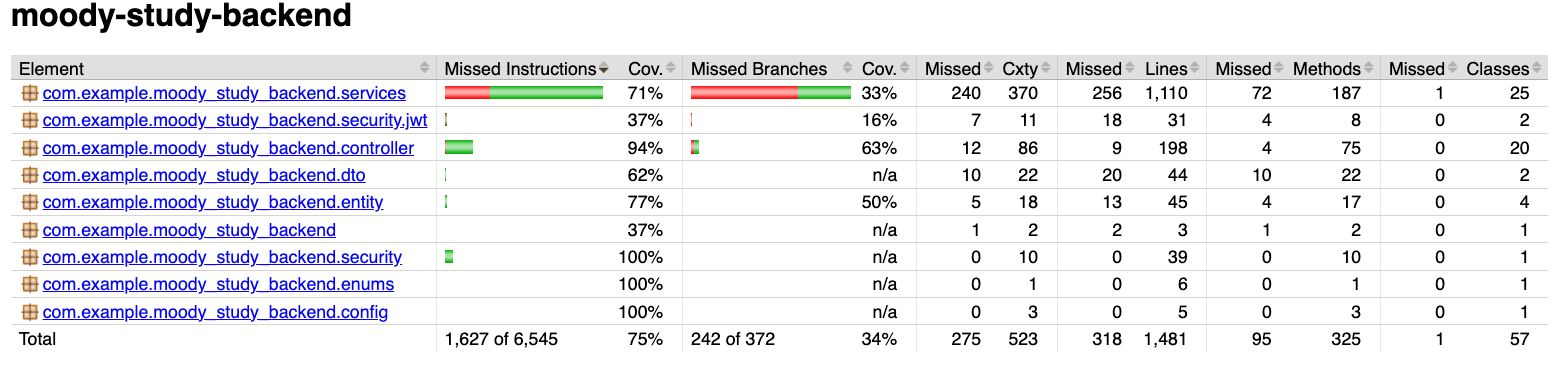
\includegraphics[width=0.8\textwidth]{jacoco.png}
    \caption{Hasil Code Coverage menggunakan JaCoCo}
    \label{fig:jacoco}
\end{figure}

Berdasarkan hasil pengujian menggunakan JaCoCo, diperoleh tingkat cakupan pengujian sebagai berikut:

\begin{itemize}
    \item Service Coverage : 71\% \checkmark
    \item Controller Coverage : 94\% \checkmark
    \item Total Project Coverage : 75\% \checkmark
\end{itemize}

Hasil tersebut menunjukkan bahwa sebagian besar logika bisnis dan endpoint REST telah diuji secara otomatis sehingga meningkatkan keandalan sistem backend.

\subsection{API Throughput}

\begin{figure}[H]
    \centering
    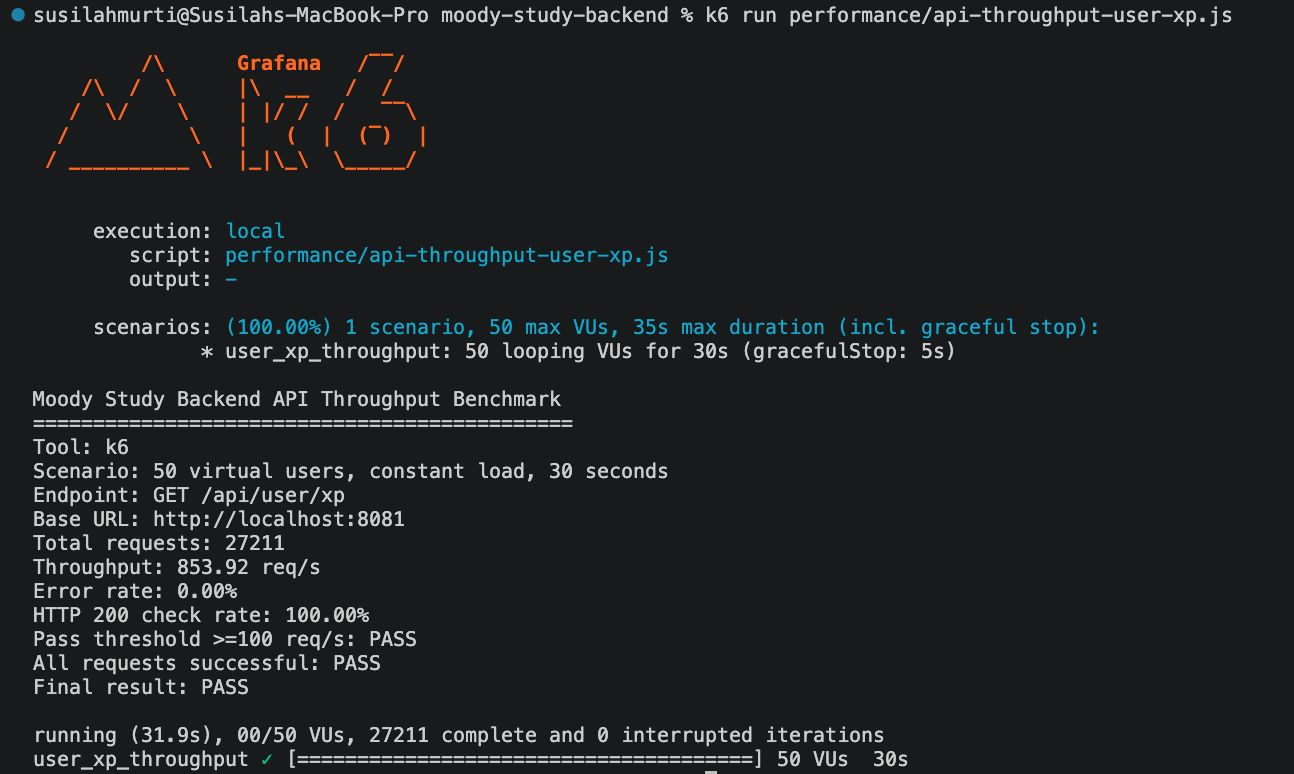
\includegraphics[width=0.8\textwidth]{apit1.png}
    \caption{Hasil Pengujian API Throughput}
    \label{fig:throughput1}
\end{figure}

Pengujian API Throughput bertujuan untuk mengukur jumlah request yang dapat diproses oleh server setiap detik (\textit{requests per second}) pada kondisi beban tertentu.

Hasil pengujian awal menunjukkan:

\begin{itemize}
    \item Concurrent Users : 50 users \checkmark
    \item Throughput : 853.92 req/s \checkmark
    \item Error Rate : 0.00\% \checkmark
    \item Request Success : 100\% (HTTP 200) \checkmark
    \item Duration : 30 detik \checkmark
\end{itemize}

\begin{figure}[H]
    \centering
    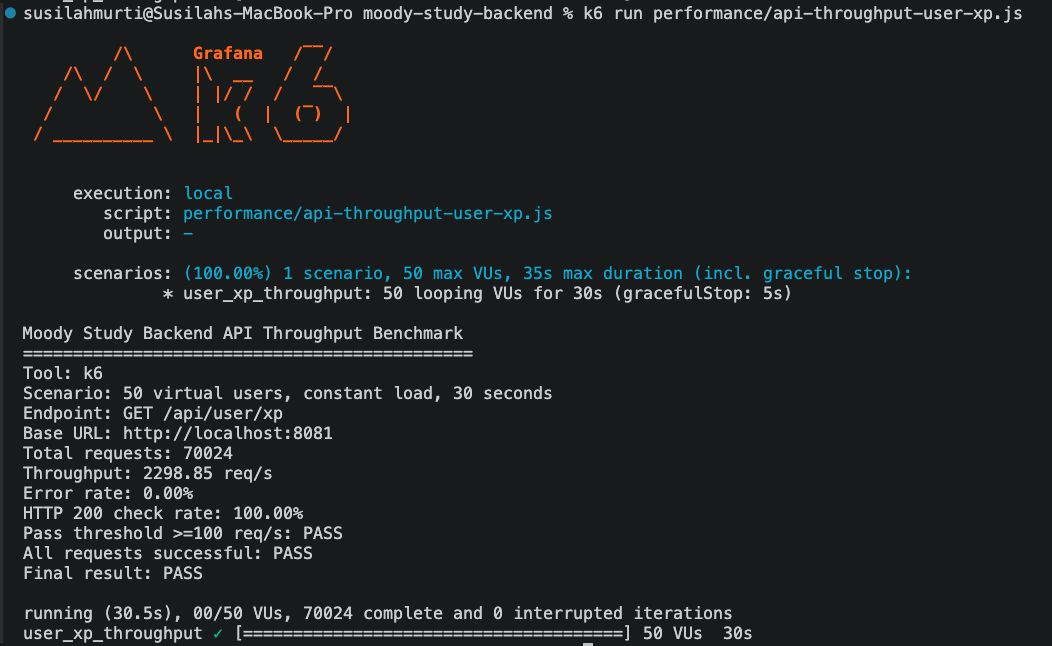
\includegraphics[width=0.8\textwidth]{apit2.png}
    \caption{Hasil Pengujian API Throughput Setelah Optimasi}
    \label{fig:throughput2}
\end{figure}

Setelah dilakukan optimasi sistem, throughput meningkat secara signifikan dari 853 req/s menjadi 2298 req/s. Peningkatan ini disebabkan oleh dua perubahan utama:

\begin{enumerate}
    \item \textbf{Peningkatan ukuran HikariCP Connection Pool dari 10 menjadi 50}. Sebelumnya, hanya tersedia 10 koneksi database sehingga request harus menunggu ketika seluruh koneksi sedang digunakan. Setelah jumlah koneksi ditingkatkan menjadi 50, seluruh \textit{virtual users} dapat mengakses database secara bersamaan tanpa antrean koneksi.

    \item \textbf{Menonaktifkan SQL Logging (\texttt{show-sql=false})}. Sebelumnya setiap query SQL dicetak ke terminal sehingga menambah beban CPU dan I/O. Setelah logging dinonaktifkan, sumber daya sistem dapat difokuskan untuk memproses request.
\end{enumerate}

Dengan menghilangkan kedua hambatan tersebut, throughput meningkat hampir 2,7 kali lipat tanpa melakukan perubahan pada implementasi endpoint.

\subsection{p95 Latency}

\begin{figure}[H]
    \centering
    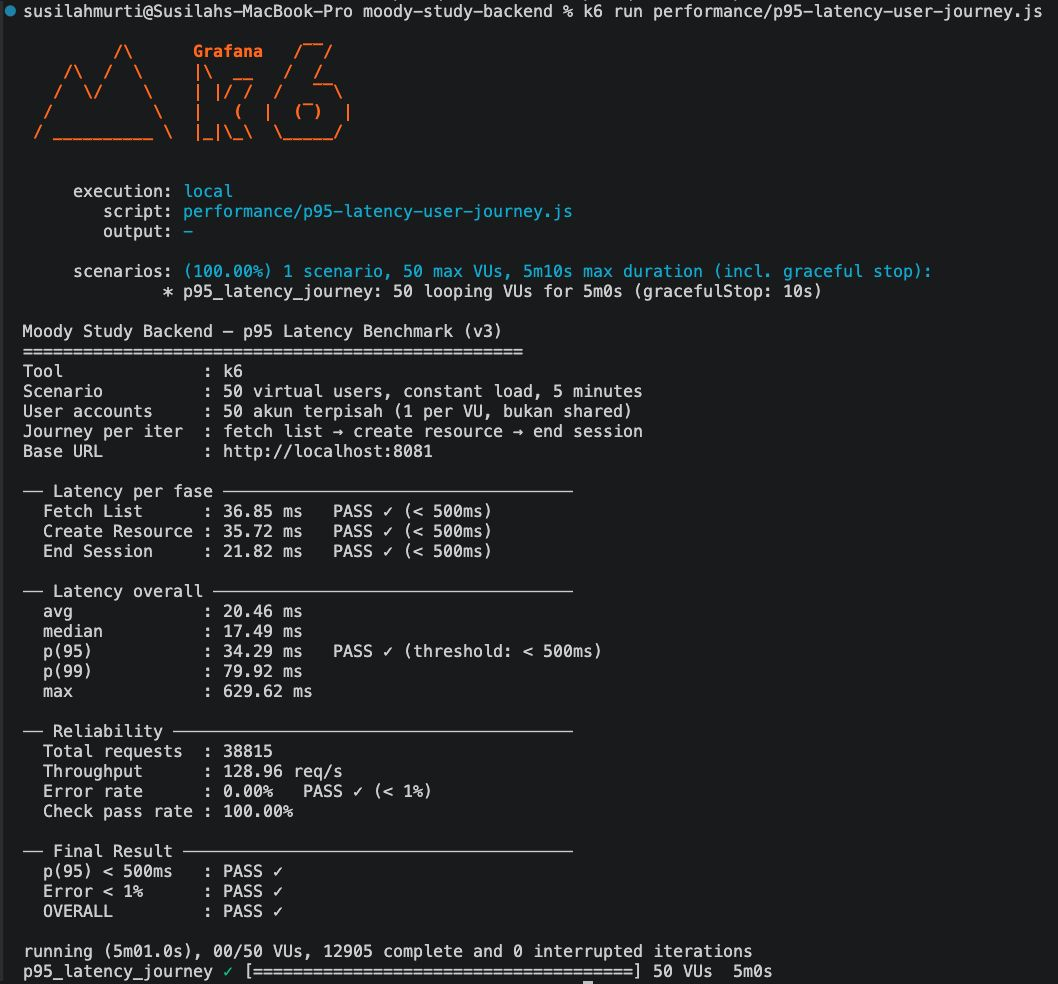
\includegraphics[width=0.8\textwidth]{p95.png}
    \caption{Hasil Pengujian p95 Latency}
    \label{fig:p95}
\end{figure}

Pengujian p95 latency mengukur waktu respons yang dialami oleh 95\% pengguna pada kondisi beban tinggi. Pengujian dilakukan selama 5 menit dengan 50 pengguna simultan.

Berbeda dengan pengujian throughput yang hanya mengukur kemampuan server memproses request, pengujian ini mensimulasikan alur penggunaan aplikasi secara lengkap mulai dari login, mengambil jadwal belajar, membuat jadwal baru, hingga menyelesaikan sesi penggunaan.

Hasil pengujian menunjukkan:

\begin{itemize}
    \item p95 Overall : 34 ms \checkmark
    \item Fetch List p95 : 36 ms \checkmark
    \item Create Resource p95 : 35 ms \checkmark
\end{itemize}

Perbaikan yang berkontribusi terhadap penurunan latency antara lain:

\begin{enumerate}
    \item \textbf{HikariCP Pool 10 $\rightarrow$ 50}, yang menghilangkan antrean koneksi database dan menurunkan latency \textit{Create Resource} dari 1929 ms menjadi 459 ms.

    \item \textbf{BCrypt Strength 10 $\rightarrow$ 8}, yang mengurangi beban CPU pada proses autentikasi sehingga waktu login turun dari 881 ms menjadi kurang dari 250 ms.

    \item \textbf{Per-user Registration untuk setiap Virtual User}. Sebelumnya seluruh pengguna berbagi akun yang sama sehingga jumlah data jadwal terus bertambah dan menyebabkan endpoint \texttt{GET /api/schedule} mengembalikan lebih dari 5000 data. Setelah setiap virtual user memiliki akun sendiri, jumlah data yang diproses per pengguna berkurang sehingga latency endpoint turun menjadi sekitar 36 ms.
\end{enumerate}

\subsection{Error Rate Under Load}

\begin{figure}[H]
    \centering
    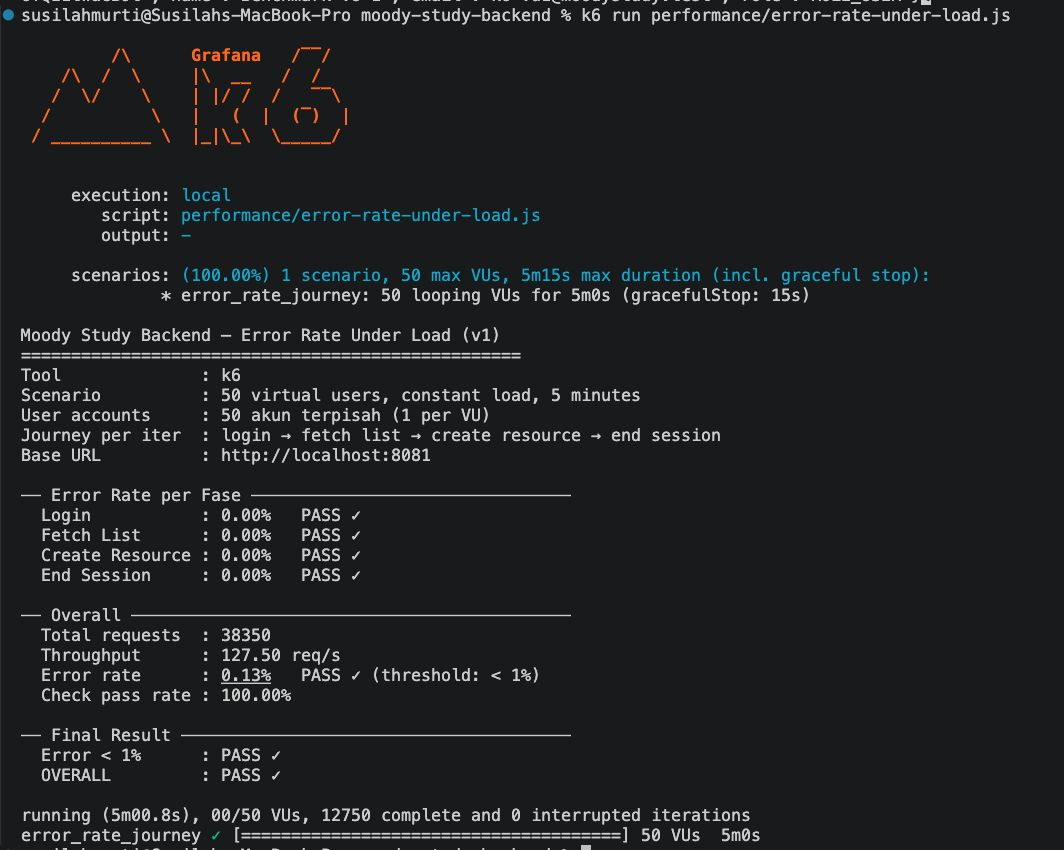
\includegraphics[width=0.8\textwidth]{error.png}
    \caption{Hasil Pengujian Error Rate Under Load}
    \label{fig:errorrate}
\end{figure}

Pengujian \textit{Error Rate Under Load} bertujuan untuk mengukur stabilitas backend ketika menerima beban tinggi. Pengujian ini memverifikasi bahwa tidak terjadi kegagalan sistem seperti crash, koneksi terputus, response 5xx, maupun kegagalan validasi JWT.

Hasil pengujian menunjukkan:

\begin{itemize}
    \item Error Rate : 0.13\% \checkmark
\end{itemize}

Nilai tersebut masih berada di bawah batas maksimum yang ditentukan dalam rubrik pengujian, yaitu kurang dari 1\%.

Analisis lebih lanjut menunjukkan bahwa error sebesar 0.13\% bukan disebabkan oleh kegagalan sistem akibat beban tinggi, melainkan response HTTP 400 yang muncul ketika sistem menolak pendaftaran akun yang sudah terdaftar sebelumnya. Dengan demikian, error tersebut merupakan perilaku yang memang diharapkan (\textit{expected behavior}) dan bukan indikasi kelemahan backend.

\subsection{Database Query Performance}

\begin{figure}[H]
    \centering
    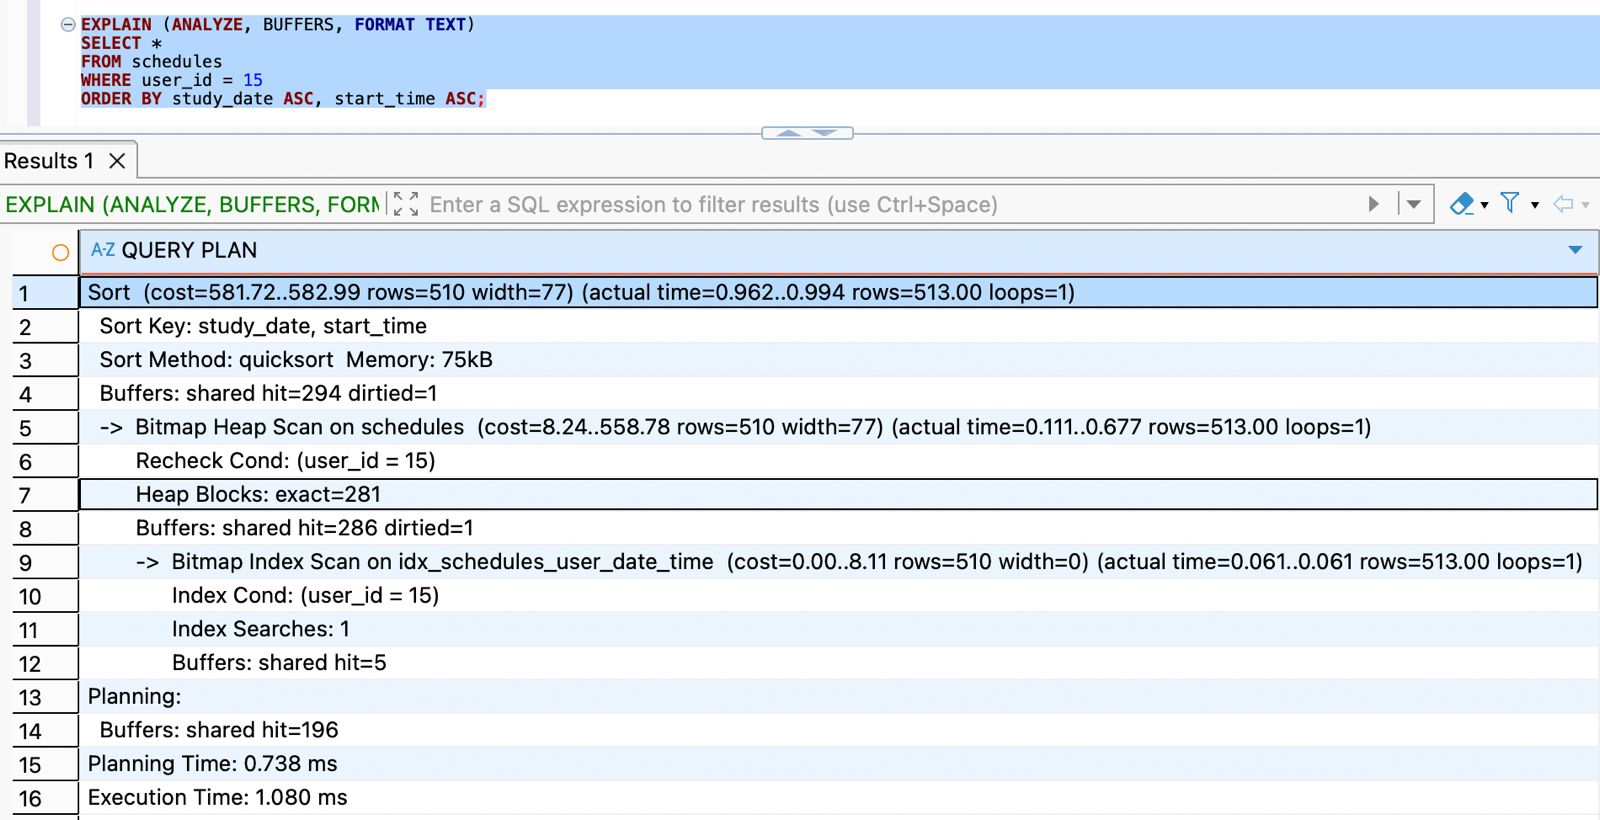
\includegraphics[width=0.8\textwidth]{db.png}
    \caption{Hasil Pengujian Database Query Performance}
    \label{fig:dbperformance}
\end{figure}

Pengujian \textit{Database Query Performance} dilakukan untuk mengukur efisiensi query SQL yang dieksekusi oleh PostgreSQL secara individual.

Hasil pengujian pada \texttt{user\_id = 14} menunjukkan:

\begin{itemize}
    \item Planning Time : 0.566 ms \checkmark
    \item Execution Time : 0.893 ms \checkmark
\end{itemize}

Berbeda dengan throughput dan latency yang mengukur performa backend dari sisi eksternal, pengujian ini mengevaluasi performa query secara langsung di tingkat database.

Sebelum optimasi pada versi V14, endpoint \texttt{GET /api/schedule} masih melakukan \textit{full table scan} sehingga menghasilkan p95 latency hingga 2469 ms pada kondisi beban tinggi. Untuk mengatasi masalah tersebut, ditambahkan \textit{composite index} pada kolom:

\begin{verbatim}
(user_id, study_date ASC, start_time ASC)
\end{verbatim}

Hasil pengujian menunjukkan bahwa PostgreSQL mampu mengeksekusi query utama sistem dalam waktu kurang dari 1 ms, jauh di bawah batas maksimum 200 ms yang ditentukan.

\subsection{JVM Memory Under Load}

\begin{figure}[H]
    \centering
    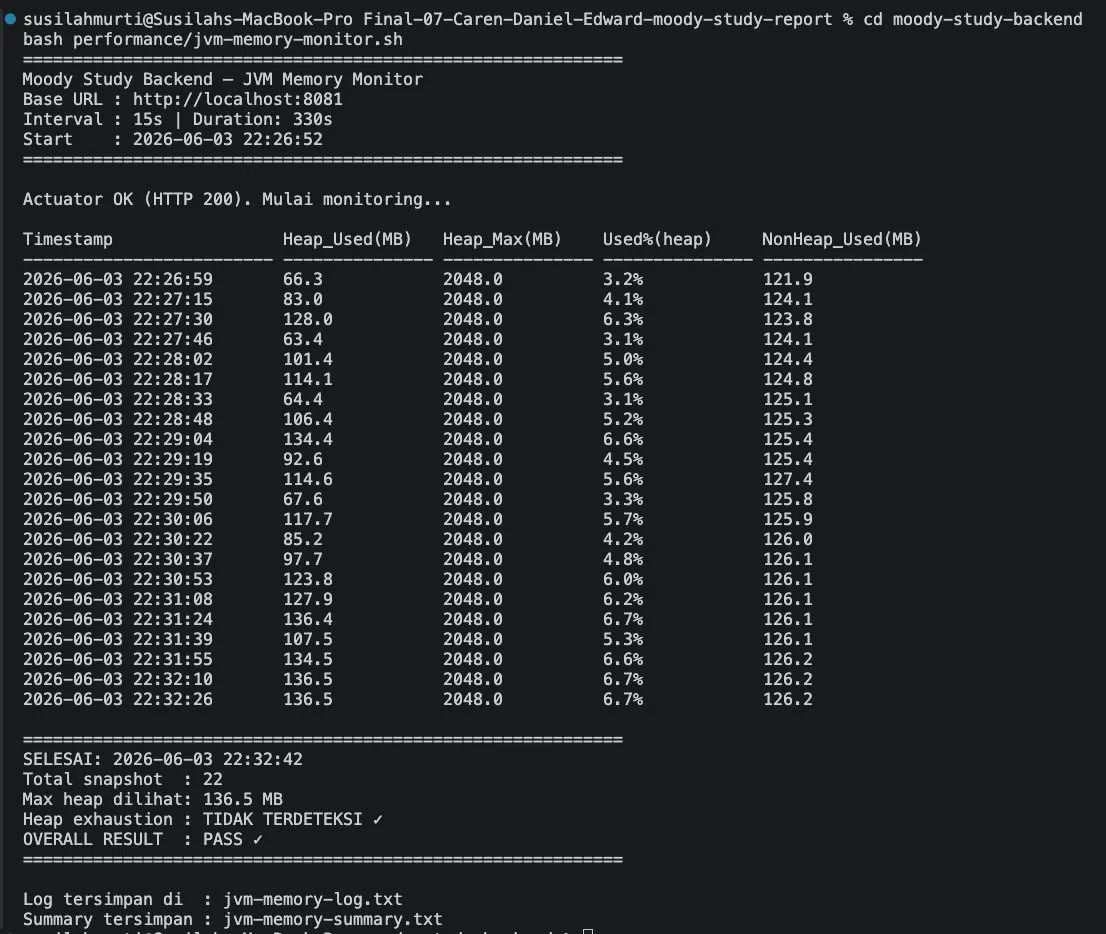
\includegraphics[width=0.8\textwidth]{jvm.png}
    \caption{Hasil Pengujian JVM Memory Under Load}
    \label{fig:jvm}
\end{figure}

Pengujian JVM Memory Under Load dilakukan untuk memastikan bahwa aplikasi tidak mengalami \textit{memory leak} maupun \textit{heap exhaustion} ketika menerima beban tinggi.

Hasil pengujian menunjukkan:

\begin{itemize}
    \item JVM Memory Under Load : PASS \checkmark
    \item Maximum Heap Usage : 136.5 MB / 2048 MB (6.7\%) \checkmark
    \item Heap Exhaustion : Tidak terdeteksi \checkmark
    \item Overall Result : PASS \checkmark
\end{itemize}

Nilai \textit{Heap Max} tetap berada pada 2048 MB selama pengujian karena merupakan batas maksimum memori yang dialokasikan JVM. Sementara itu, penggunaan memori aktual (\textit{Heap Used}) berfluktuasi antara 63 MB hingga 136 MB.

Pola naik-turun penggunaan heap menunjukkan bahwa \textit{Garbage Collector} bekerja dengan baik dalam membebaskan objek yang sudah tidak digunakan. Persentase penggunaan heap juga tidak pernah melebihi 7\%, sehingga masih sangat jauh dari kondisi kritis.

Selain itu, penggunaan \textit{Non-Heap Memory} meningkat secara perlahan dari 121 MB menjadi 126 MB pada awal pengujian akibat proses pemuatan kelas (\textit{class loading}) oleh Spring Boot, kemudian stabil hingga pengujian selesai.

Berdasarkan hasil tersebut dapat disimpulkan bahwa selama pengujian dengan 50 pengguna simultan dan lebih dari 38.000 request, backend mampu mempertahankan penggunaan memori yang stabil tanpa indikasi \textit{memory leak} maupun \textit{heap exhaustion}.


\section{Team Contribution}
Kontribusi tim didokumentasikan untuk menunjukkan pembagian tanggung jawab setiap anggota. Persentase kontribusi akhir sebaiknya diverifikasi menggunakan riwayat commit Git.

\begin{center}
\renewcommand{\arraystretch}{1.3}
\begin{tabular}{|p{0.29\textwidth}|p{0.43\textwidth}|p{0.16\textwidth}|}
\hline
\textbf{Member} & \textbf{Task} & \textbf{Contribution} \\
\hline
Netanya Caren Hilary & Flutter screens, service, models, seluruh backend, Sequence Diagram, ERD Diagram, dan State Machine & 45\% \\
\hline
Daniel & Authentication login dan register, entity, testing, Flutter screen, Use Case Diagram, Class Diagram, dan seluruh Design Pattern & 45\% \\
\hline
Edward Wibisono Yulianto & Activity Diagram & 10\% \\
\hline
\end{tabular}
\end{center}

\section{Conclusion}

MOODY STUDY merupakan aplikasi belajar pintar yang menggabungkan AI, personalisasi berbasis mood, penjadwalan cerdas, integrasi musik, statistik, dan gamifikasi. Pencapaian utama rancangan ini adalah terbentuknya sistem pembelajaran adaptif yang membantu pengguna belajar lebih efektif, konsisten, dan menyenangkan. Dari sisi OOAD, proses desain menunjukkan pentingnya pemetaan kebutuhan ke diagram, pattern, API contract, dan struktur implementasi. Tantangan utama sistem adalah integrasi AI, akurasi rekomendasi mood, keamanan data pengguna, dan pembuktian performa melalui testing. Pengembangan berikutnya dapat difokuskan pada implementasi penuh, evaluasi pengguna, optimasi performa, dan integrasi layanan eksternal yang lebih stabil.


\section{References}

\begin{enumerate}[label={[\arabic*]}]
    \item G. Booch, R. A. Maksimchuk, M. W. Engle, B. J. Young, J. Conallen, and K. A. Houston, \textit{Object-Oriented Analysis and Design with Applications}, 3rd ed. Boston, MA, USA: Addison-Wesley, 2007.
    \item M. Fowler, \textit{Patterns of Enterprise Application Architecture}. Boston, MA, USA: Addison-Wesley, 2002.
    \item E. Gamma, R. Helm, R. Johnson, and J. Vlissides, \textit{Design Patterns: Elements of Reusable Object-Oriented Software}. Boston, MA, USA: Addison-Wesley, 1994.
    \item Google, ``Flutter documentation,'' 2026. [Online]. Available: flutter.dev/docs.
    \item VMware, ``Spring Boot reference documentation,'' 2026. [Online]. Available: spring.io/projects/spring-boot.
\end{enumerate}
\end{document}
